\documentclass[12pt]{extarticle}
\usepackage[utf8]{inputenc}
\usepackage{amsmath}
\usepackage{lmodern}
% \usepackage[square,numbers]{natbib}
\usepackage{graphicx}
\usepackage{tikz}
\usepackage{pdfpages}
\usepackage[ngerman]{babel}
\usepackage{caption}
\usepackage{subcaption}
\usepackage{tocbibind}
\usepackage{hyperref}
% \usepackage{cleveref}
% cleveref sorgt für Probleme mit acronym

%\usepackage{geometry}
\usepackage[onehalfspacing]{setspace}
\usepackage{color}
\usepackage{attachfile}
\usepackage[explicit]{titlesec}
\usepackage{lipsum}
\usepackage{blindtext,listings}
% \usepackage{float}
% \usepackage{textcomp}
\usepackage{microtype} %gegen flattersatz
\usepackage[printonlyused]{acronym} %Abkürzungen
\usepackage{float}
\usepackage{booktabs}
\usepackage{eurosym}
\usepackage{glossaries}
\usepackage{fancyhdr} %Header Paket
\usepackage[toc,page]{appendix}


% Hinweis Box
\usepackage[T1]{fontenc} 
\usepackage{blindtext} 
\usepackage{xcolor} 
\usepackage{framed} 

% Automatische Absaätze
\usepackage{parskip}

% % Literatur
\usepackage[backend=bibtex,style=numeric-comp,sorting=none]{biblatex}
\addbibresource{references.bib}

% Hinweis-Box
\usepackage{tcolorbox}
%Tabellen
\usepackage{booktabs}
\usepackage{multirow}
\usepackage{ltablex}
\usepackage{rotating}
\usepackage{tabularray}
\usepackage{makecell}
\usepackage{adjustbox} 
%----------Code listings------------
\usepackage{listings}
% Farben definieren
\definecolor{numb}{rgb}{0.0, 0.5, 0.0}
\definecolor{string}{rgb}{0.4, 0.0, 0.4}
\definecolor{background}{HTML}{F5F5F5}
\definecolor{darkgray}{gray}{0.2}
\lstdefinelanguage{json}{
    numbers=left,
    numberstyle=\small,
    backgroundcolor=\color{background},
    numbersep=8pt,
    frame=single,
    rulecolor=\color{black},
    showspaces=false,
    showtabs=false,
    breaklines=true,
    postbreak=\raisebox{0ex}[0ex][0ex]{\ensuremath{\color{gray}\hookrightarrow\space}},
    breakatwhitespace=true,
    basicstyle=\ttfamily\small,
    lineskip=-0.25pt, 
    upquote=true,
    morestring=[b]",
    stringstyle=\color{darkgray},
    literate=
     *{0}{{{\color{numb}0}}}{1}
      {1}{{{\color{numb}1}}}{1}
      {2}{{{\color{numb}2}}}{1}
      {3}{{{\color{numb}3}}}{1}
      {4}{{{\color{numb}4}}}{1}
      {5}{{{\color{numb}5}}}{1}
      {6}{{{\color{numb}6}}}{1}
      {7}{{{\color{numb}7}}}{1}
      {8}{{{\color{numb}8}}}{1}
      {9}{{{\color{numb}9}}}{1}
      {\{}{{{\color{black}{\{}}}}{1}
      {\}}{{{\color{black}{\}}}}}{1}
      {[}{{{\color{black}{[}}}}{1}
      {]}{{{\color{black}{]}}}}{1},
}
%%% inline %%%
\tcbset{inlinebox/.style={
  on line,
  box align=base,
  colback=gray!20,
  colframe=gray!50,
  boxrule=0.5pt,
  arc=2pt,
  top=1pt,
  bottom=1pt,
  left=2pt,
  right=2pt
}}
%%% inline %%%
%----------Code listings------------

%----------Farben-------------------
\definecolor{swaggerget}{HTML}{61affe}
\definecolor{swaggerpost}{HTML}{49cc90}
\definecolor{swaggerput}{HTML}{fca130}
\definecolor{swaggerdelete}{HTML}{f93e3e}
\definecolor{babyblue}{HTML}{F2F5FD}
\definecolor{DynamischesSubmodel}{HTML}{FFF2CC}
% \definecolor{tableHeader}{HTML}{d8e4fc}
\definecolor{tableHeader}{RGB}{230,230,230}
\definecolor{rowHeader}{RGB}{245,245,245} 
%----------Farben-------------------

%----------Aufzählung-------------------
\usepackage{enumitem}
\usepackage{pifont}
\usepackage{amssymb}
\definecolor{orangeHaken}{HTML}{aa7e5e}
\definecolor{greenHaken}{HTML}{49cc90}

\newcommand{\recommended}{\textcolor{orangeHaken}{\ding{52}}} % orange Kreis
\newcommand{\optional}{\textcolor{black}{\ding{118}}}
\newcommand{\notused}{\textcolor{black}{\ding{55}}}     % X-Symbol
\newcommand{\mandatory}{\textcolor{DynamischesSubmodel}{\ding{51}}} % grüner Haken

%%% legende %%%
\tcbset{legendbox/.style={
  colback=background,
  colframe=white,
  arc=2mm,
  boxrule=0pt,
  left=2mm,
  right=2mm,
  top=1mm,
  bottom=1mm,
  boxsep=4pt,
  width=\textwidth
}}
%----------Aufzählung-------------------
\usepackage[a4paper, asymmetric, left=3cm,right=3cm,top=1cm,bottom=1.5cm,includeheadfoot, headheight=40pt]{geometry}

\pagestyle{plain} %nur Seitenzahl in der Fußzeile (LaTeX-Standard)


\renewcommand*{\listoffigures}{%
  \begingroup
  \tocchapter
  \tocfile{\listfigurename}{lof}
  \endgroup
  
  
}

% Befehl zum Schreiben von Quellenangeben in Bildern
\newcommand*{\quelle}{%
    \vspace{2mm}
    \footnotesize Quelle:
}


\loadglsentries{glossary}


\makeglossaries

% 4. Unterpunkt
\setcounter{secnumdepth}{4}
\setcounter{tocdepth}{4}

\begin{document}

\begin{titlepage}

\begin{singlespace}
    
\begin{tikzpicture}[remember picture, overlay]
     \node [shift={(-17 cm,-2.25cm)}]  at (current page.north east)
         {
            
\includegraphics[height=1.4cm]{./Bilder/groninger_Logo_Transparent_RGB.png}
         };
\end{tikzpicture}
 \begin{tikzpicture}[remember picture, overlay]
     \node [shift={(-3.5 cm,-2.5cm)}]  at (current page.north east)
         {
             
\includegraphics[height=2.5cm]{./Bilder/HHN.png}
         };
 \end{tikzpicture}




\vspace{1cm}
\centering
\fontsize{30}{32} \selectfont Implementierung eines digitalen Zwillings für die robocell und Evaluierung eines KI gestützten Konzepts zur Optimierung  
 \par
\vspace{1.5cm}
\fontsize{36}{33} \selectfont Bachelorarbeit \par
\vspace{1.5cm}
\fontsize{16}{20} \selectfont Studiengang Elektrotechnik, SPO 03\\
Hochschule Heilbronn, Campus Künzelsau
\vspace{1.5cm}

\fontsize{18}{22} \selectfont von \par
\fontsize{20}{25} \selectfont Albert Heinke\par
\vspace{1.5cm}
\fontsize{18}{22} \selectfont 01. September 2025 \par
\vfill

\fontsize{13}{18} \selectfont
\begin{tabular}{ l  l }
  Bearbeitungszeitraum & \hspace{0.85cm} 4 Monate \\
  Matrikelnummer, Semester & \hspace{0.85cm} 212081, 8. Fachsemester \\
  Unternehmen, Ort & \hspace{0.85cm} groninger \& co. GmbH, Crailsheim \\
  Betrieblicher Betreuer & \hspace{0.85cm} Jan Völkl, M.Sc. \\
  Erstprüfer & \hspace{0.85cm} Prof. Dr.-Ing. Ralf Gessler \\
  Zweitprüfer & \hspace{0.85cm} Prof. Dr.-Ing. Marcus Stolz \\
\end{tabular}

\newpage


%\pagenumbering{gobble}

\pagenumbering{Roman}
\setcounter{page}{2}

\renewcommand{\contentsname}{Inhaltsverzeichnis}

\fontsize{11}{18} \selectfont

\end{singlespace}
\end{titlepage}
% pdf zur Tätigkeitsübersicht
% pdf zur studentischer Reflexion


\newpage
\setcounter{page}{2}

%\includepdf{Deckblatt/sperrvermerk.pdf} 

%\includepdf{Deckblatt/ehrenwoertlErklaerung.pdf} 
% nach Unterschreiben der von Sperrvermerk und ehrenwörtlicher Erklärung, hier als eingescanntes PDF einfügen und Latexteil auskommentieren

\subsection*{Sperrvermerk}
Die vorliegende Arbeit beinhaltet interne vertrauliche Informationen des Unternehmens groninger \& Co. GmbH. Sie ist nur für die Beteiligten am Begutachtungs- und Evaluationsprozess bestimmt. Die Weitergabe des Inhalts der Arbeit im Gesamten oder in Teilen sowie das Anfertigen von Kopien oder Abschriften – auch in digitaler Form – sind grundsätzlich untersagt. Ausnahmen bedürfen der schriftlichen Genehmigung des Unternehmens groninger \& Co. GmbH. \\ \\ \\ \\

\hspace{2cm}
\parbox{9cm}{\centering \hrule
\strut \centering\footnotesize Name, Vorname des Betreuers/Gutachters/Prüfers \\ (Bitte in Druckbuchstaben)} \\ \\ \\

\parbox[t][][t]{5cm}{\centering Crailsheim, \today \hrule \strut \centering \footnotesize Ort, Datum} %\hfill
\hspace{3cm}
\parbox[t][][t]{5cm}{\vspace{0.09cm} \hrule \strut \centering \footnotesize  Unterschrift des Betreuer/Gutachter/Prüfer}

\input{ehrenwoertlichErklärung.tex}


\newpage
\begin{spacing}{1.0}
\tableofcontents %Inhaltsverzeichnis
\newpage
\end{spacing}

\begin{spacing}{1.0}
  \section*{Abkürzungsverzeichnis}
\begin{singlespacing}
\end{singlespacing}
\begin{acronym}

\acro{aas}[AAS]{Asset Administration Shell}

\acro{assetid}[Asset-ID]{Asset Identifier}

\acro{bom}[BOM]{Bill of Material}

\acro{cad}[CAD]{Computer Aided Design}

\acro{dpp}[DPP]{Digitaler Produktpass}
\acroplural{dpp}[DPPs]{Digitale Produktpässe}

\acro{erp}[ERP]{Enterprise Resource Planing}

\acro{idta}[IDTA]{Industrial Digital Twin Association}

\acro{ki}[KI]{Künstliche Intelligenz}

\acro{mes}[MES]{Manufacturing Execution System}

\acro{opcua}[OPC UA]{Open Platform Communications Unified Architecture}

\acro{plm}[PLM]{Product Lifecycle Management}

\acro{rami}[RAMI 4.0]{Referenzarchitekturmodell Industrie 4.0}

\end{acronym}



\newpage
  \newpage
  \end{spacing}

\listoffigures
\newpage

\listoftables
\newpage

\lstlistoflistings 

\newpage
\thispagestyle{empty}
\cleardoublepage

\pagenumbering{arabic}
%arabische Seitenzahlen im Hauptteil

\pagestyle{fancy}
\fancyhf{}
\renewcommand{\headrulewidth}{0.4pt} %obere Trennlinie
\renewcommand{\sectionmark}[1]{\markright{\arabic{section}.\ #1}}
\renewcommand{\subsectionmark}[1]{}

\renewcommand{\footrulewidth}{0.4pt}% default is 0pt

\fancyhead[LE, RO]{\rightmark}

\fancyfoot[LE, RO]{\thepage}% Seitenzahl in Fußzeile (Links auf ungeraden LO und Rechts auf geraden Seiten RE) 
%\fancyfoot[LE, RO]{Albert Heinke 2025}% Name und Jahreszahl in Fußzeile (Links auf geraden LE und Rechts auf ungeraden Seiten RO)

\input{commands.tex}
%=======================BEGIN HAUPTTEIL===================================%
\thispagestyle{fancy}
\section{Einleitung}
\subsection{Motivation}
\label{sec:Motivation}
Im Zuge der vierten industriellen Revolution gewinnen digitale Zwillinge zunehmend an Bedeutung. 
Sie ermöglichen die digitale Abbildung physischer Assets und schaffen damit die Grundlage für transparentere und effizientere industrielle Prozesse. 
Viele Unternehmen setzen bereits auf solche digitalen Abbilder, verwenden dabei jedoch häufig proprietäre Lösungen, die nicht interoperabel sind und den Austausch von Daten über System- und Unternehmensgrenzen hinweg erschweren.

Mit der steigenden Nachfrage nach digitalen Zwillingen wächst der Bedarf an standardisierten und herstellerunabhängigen Lösungen. 
Als Antwort auf diese Herausforderung hat die Plattform Industrie 4.0 die sogenannte \ac{aas} etabliert. 
Sie bietet ein einheitliches Rahmenwerk zur interoperablen Umsetzung digitaler Zwillinge und erlaubt es, Informationen zu einem Asset über dessen gesamten Lebenszyklus hinweg digital zu erfassen und strukturiert bereitzustellen.

Die zunehmende Umsetzung der \acs{aas} in Pilotprojekten sowie erste produktive Anwendungen verdeutlichen ihre hohe Relevanz und das Potenzial für die industrielle Praxis. 
Gleichzeitig führen regulatorische Vorgaben wie der von der EU geplante digitale Produktpass (\acs{dpp}), der künftig für zahlreiche Produktgruppen verpflichtend sein wird, die Notwendigkeit eines standardisierten und semantisch eindeutigen Informationsmodells deutlich vor Augen.
Vor diesem Hintergrund gewinnt die Auseinandersetzung mit der \acs{aas} für Unternehmen bereits heute an Bedeutung, um den steigenden Anforderungen an Transparenz, Rückverfolgbarkeit und Effizienz gerecht zu werden.

\subsection{Zielsetzung}

Ziel dieser Arbeit ist es, am Beispiel des Abfüll- und Verschließmoduls der robocell-Linie der Firma groninger das Potenzial der \acs{aas} für die Modellierung eines digitalen Zwillings zu untersuchen. 
Der Fokus liegt dabei auf dem Mehrwert, den die \acs{aas} insbesondere in Bezug auf Interoperabilität, Produktivität und Nachverfolgbarkeit bieten kann. 

Interoperabilität bezeichnet in diesem Zusammenhang die standardisierte und herstellerunabhängige Vernetzung von Maschinen und Systemen, die einen konsistenten Datenaustausch innerhalb und zwischen Unternehmen ermöglicht. 
Produktivität umfasst die effiziente Bereitstellung von Informationen, die Optimierungspotenziale für betriebliche Prozesse eröffnet. 
Nachverfolgbarkeit umfasst die lückenlose Erfassung relevanter Asset-Daten über den gesamten Lebenszyklus, wodurch Zustandsänderungen transparent und nachvollziehbar werden.

Darüber hinaus soll das Potenzial von Künstlicher Intelligenz (\acs{ki}) zur Analyse und Nutzung der im digitalen Zwilling erfassten Daten betrachtet werden, um mögliche Optimierungsansätze im Betrieb aufzuzeigen. 
Ebenso soll die Praxistauglichkeit der eingesetzten Open-Source-Lösungen zur Modellierung und Bereitstellung der AAS untersucht werden.
Die gewonnenen Erkenntnisse dienen als Grundlage für eine Handlungsempfehlung, die Nutzen und Relevanz des Einsatzes der \acs{aas} im konkreten Anwendungskontext bei groninger bewertet.

\subsection{Vorgehensweise}

Die Arbeit beginnt mit einer Darstellung der theoretischen Grundlagen (Kapitel \ref{sec:Grundlagen}). 
Dazu gehören zentrale Konzepte wie \acs{ki}, der digitale Zwilling sowie insbesondere die \acs{aas}, die allesamt eine zentrale Rolle im Rahmen von Industrie 4.0 einnehmen. 
Darüber hinaus werden mit dem Package Explorer, Eclipse BaSyx und OPC~UA für die weitere Vorgehensweise relevante Werkzeuge und Technologien eingeführt, die die methodische Basis für die anschließende Entwicklung bilden.

Darauf aufbauend wird in Kapitel \ref{sec:Entwicklung} der digitale Zwilling für das Abfüll- und Verschließmodul der robocell prototypisch implementiert. 
Dies umfasst sowohl die Modellierung der AAS als auch ihre Integration in ein Industrie-4.0-kompatibles System, das durch die Anbindung dynamischer Datenquellen erweitert wird. 
Außerdem wird ein Verfahren zur Anomalieerkennung mithilfe von \acs{ki} konzipiert und prototypisch implementiert. 
Abschließend werden mit dem \acs{dpp} sowie der automatisierten Generierung von AAS zwei praxisnahe Anwendungsfälle ausgearbeitet.

Im Ergebnisteil (Kapitel \ref{sec:Ergebnisse}) wird der entwickelte \acs{aas}-Demonstrator vorgestellt, das \acs{ki}-Modell evaluiert und die beiden Anwendungsfälle reflektiert. 
Zudem wird eine Bewertung der eingesetzten Werkzeuge hinsichtlich ihrer Praxistauglichkeit vorgenommen.

Kapitel \ref{sec:Zusammenfassung} fasst die zentralen Ergebnisse der Arbeit zusammen, leitet eine Handlungsempfehlung für das Unternehmen groninger ab und schließt mit einem Ausblick auf mögliche Weiterentwicklungen.

\newpage
\section{Grundlagen}
\label{sec:Grundlagen}
Das folgende Kapitel stellt die theoretischen und technologischen Grundlagen vor, die für das Verständnis und die Umsetzung dieser Arbeit erforderlich sind.
Es beginnt mit einer Einführung in die Industrie 4.0, und vermittelt ein grundlegendes Verständnis für das Konzept des digitalen Zwillings.
Anschließend werden die Struktur und Funktion der \acs{aas} sowie die Rolle des \acs{dpp} erläutert.
Den Abschluss bilden die technologischen Voraussetzungen für die praktische Umsetzung, darunter beispielsweise die Open-Source-Plattform Eclipse BaSyx oder der Kommunikationsstandard \ac{opcua}.
\subsection{Industrie 4.0}
% Nach der dritten industriellen Revolution, die vor allem durch den Einsatz elektronischer Systeme sowie der Informations -und Kommunikationstechnologie zur Automatisierung gekennzeichnet ist, vollzieht sich aktuell ein neuer technologischer Wandel, die vierte industrielle Revolution.
% Besser bekannt als Industrie 4.0, beschreibt sie die umfassende Vernetzung und Integration der physischen mit der digitalen Welt durch den Einsatz Cyber-physischer Systeme.

Der Begriff Industrie 4.0 wurde erstmals im Jahr 2011 im Rahmen eines von der deutschen Bundesregierung initiierten Zukunftsprojekts eingeführt, das auf die Förderung der Informatisierung in der industriellen Fertigung/Produktion abzielt.
Angestrebt wird eine Stärkung der Wettbewerbsfähigkeit der deutschen Industrie sowie eine Verbesserung der Marktposition deutscher Unternehmen im globalen Wettbewerb.

Industrie 4.0 steht dabei für die vierte industrielle Revolution und beschreibt die umfassende digitale Transformation industrieller Wertschöpfungsprozesse. 
Im Zentrum steht die intelligente Vernetzung von Menschen, Maschinen und Produkten über moderne digitale Kommunikationsnetzwerke, durch die eine weitreichende Integration der physischen mit der digitalen Welt ermöglicht wird.

Zur besseren Einordnung von Industrie 4.0 ist ein Blick auf die vorangegangenen industriellen Revolutionen hilfreich.
Die Industrialisierung begann bereits Mitte des 18. Jahrhunderts in Großbritannien und breitete sich von dort an weltweit aus. 
Mit der Entwicklung der ersten Dampfmaschine setzte die erste industrielle Revolution ein. 
Sie ermöglichte erstmals die Mechanisierung der Fertigung durch den Einsatz von Arbeits- und Kraftmaschinen. 
Dadurch konnten manuelle Tätigkeiten zunehmend durch Maschinenkraft ersetzt werden, insbesondere in der Textil-, Eisen- und Stahlindustrie, die zu den ersten Branchen gehörten, die von dieser Entwicklung profitierten.

Die zweite industrielle Revolution setzte gegen Ende des 19. Jahrhunderts ein und war maßgeblich durch den flächendeckenden Einsatz von Elektrizität geprägt. 
Mit der Erfindung elektrischer Antriebe und des Verbrennungsmotors konnten Maschinen nun auch dezentral betrieben werden. Sie waren nicht länger auf zentrale Kraftquellen wie Dampfmaschinen angewiesen. 
Dies ermöglichte eine flexiblere Gestaltung von Produktionsstätten und führte zur Entwicklung einer arbeitsteiligen Massenproduktion mithilfe von Fließ- und Förderbändern.

Ausgehend von dem deutschen Wirtschaftswunder in den sechziger Jahren des 20. Jahrhunderts entstand in den folgenden Jahrzehnten die dritte industrielle Revolution.
Diese zeichnet sich vor allem durch den Einsatz elektronischer Systeme sowie der Informations- und Kommunikationstechnologie zur Automatisierung aus und ist noch bis heute wirksam.

Aufbauend auf den vorangegangenen industriellen Revolutionen strebt die vierte industrielle Revolution eine tiefgreifende Transformation industrieller Produktionsprozesse an. 
Im Fokus steht dabei die Vernetzung von Systemen, die über moderne Internettechnologien miteinander kommunizieren.
Ziel dieser Entwicklung ist es, die industrielle Wertschöpfung deutlich flexibler und effizienter zu gestalten sowie eine stärkere Individualisierung von Produkten zu ermöglichen. 
\cite{Industrie4.0ProduktionAutomatisierung}\cite{EinführungundUmsetzungI4.0}

Trotz der weiten Verbreitung des Begriffs Industrie 4.0 mangelt es in der Literatur und Forschung an einer einheitlichen Definition.
Vor diesem Hintergrund nimmt insbesondere die Plattform Industrie 4.0 \cite{plattform_i40} eine zentrale Rolle in Deutschland ein. 
Dabei handelt es sich um eine gemeinsame Initiative des Bundesministeriums für Wirtschaft und Energie, des Bundesministeriums für Forschung, Technologie und Raumfahrt sowie führender Industrieverbände, Unternehmen, Forschungseinrichtungen und Gewerkschaften, darunter etwa der Verband Deutscher Maschinen- und Anlagenbau (VDMA), der Bundesverband Informationswirtschaft, Telekommunikation und neue Medien (Bitkom) und der \ac{zvei}.

Die Plattform ist maßgeblich an der inhaltlichen und strategischen Ausarbeitung der Industrie 4.0 beteiligt und leistet einen entscheidenden Beitrag zur Begriffsdefinition. 
Sie definiert Industrie 4.0 als
\glqq die vierte industrielle Revolution, einer neuen Stufe der Organisation und Steuerung der gesamten Wertschöpfungskette über den Lebenszyklus von Produkten.
Dieser Zyklus orientiert sich an den zunehmend individualisierten Kundenwünschen und erstreckt sich von der Idee, dem Auftrag über die Entwicklung und Fertigung, die Auslieferung eines Produkts an den Endkunden bis hin zum Recycling, einschließlich der damit verbundenen Dienstleistungen.
Basis ist die Verfügbarkeit aller relevanten Informationen in Echtzeit durch Vernetzung aller an der Wertschöpfung beteiligten Instanzen sowie die Fähigkeit aus den Daten den zu jedem Zeitpunkt optimalen Wertschöpfungsfluss abzuleiten. 
Durch die Verbindung von Menschen, Objekten und Systemen entstehen dynamische, echtzeitoptimierte und selbst organisierende, unternehmensübergreifende Wertschöpfungsnetzwerke, die sich nach unterschiedlichen Kriterien wie beispielsweise Kosten, Verfügbarkeit und Ressourcenverbrauch optimieren lassen \grqq~\cite[S. 8]{plattform_i40_definition}.

Die Definition der Plattform Industrie 4.0 verdeutlicht: Industrie 4.0 steht für einen grundlegenden Wandel in der industriellen Wertschöpfung.
Im Zentrum stehen dabei nicht nur neue technologische Möglichkeiten, sondern vor allem das Potenzial, Produktions- und Geschäftsprozesse flexibler, effizienter und nachhaltiger zu gestalten.
Durch die intelligente Vernetzung und die Nutzung von Echtzeitdaten enstehen selbstorganisierende Systeme, die auch über Unternehmensgrenzen hinweg kooperieren und tiefgreifende organisatorische Veränderungen erfordern.
Auf diese Weise werden nicht nur Qualität und Transparenz gesteigert, sondern auch Resourcen geschont und Kosten reduziert.
Insgesamnt trägt Industrie 4.0 somit nicht nur zur Verbesserung der Wirtschaftlichkeit bei, sondern leistet auch einen wichtigen Beitrag zur ökologischen Nachhaltigkeit.


% Obwohl Industrie 4.0 häufig als neuartiges Konzept dargestellt wird, basiert es im Kern auf Ideen, die schon seit mehreren Jahrzenten exisiteren.
% Bereits seit den 1980er-Jahren wurden mit Ansätzen wie dem Computer Integrated Manufacturing (CIM) oder der intelligenten Fabrik (Smart Factory) Strategien entwickelt, die auf eine computerintegrierte und automatisierte Produktion abzielen und dabei den Menschen mehr in den Hintergrund rücken.
% Allerdings scheiterten diese frühen Ansätze oft an den technische Möglichkeiten der damaligen Zeit, vor allem fehlte die Infrastruktur, Rechenleistung und Vernetzung.
% Erst mit dem technologischen Fortschritt, insbesondere der Einführung des Internetprotokolls V6 im Jahr 2012, wurde die Grundlage für eine globale, skalierbare Vernetzung von Maschinen, Produkten und Menschen im Sinne des Internet of Things geschaffen.
% Dies ermöglichte erstmals die Realisierung des Internet der Dinge (Internet of Things (IoT)), welches die technologische Basis für die Industrie 4.0 bildet.

\subsection{Künstliche Intelligenz}
% Künstliche Intelligenz ist eine Schlüsselkomponente der Industrie 4.0.
Mit der zunehmenden Vernetzung von Maschinen und Anlagen entstehen immer größere Datenmengen entlang von Produktionsprozessen.
Diese Daten bieten enorme Potenziale zur Optimierung industrieller Abläufe, beispielsweise zur Steigerung der Anlagenverfügbarkeit, zur Reduzierung von Ausschuss oder zur Verbesserug der Produktqualität.
Zudem erlauben intelligente Produkte, das Hersteller auch während der Nutzungsphase Informationen über den Einsatz und Zustand eines Produktes erhalten.
Auf Basis dieser lassen sich neue Dienstleistungen und Anwendungen entwickeln, wie etwa die vorrauschaunde Instandhaltung oder die dynamische Optimierung von Betriebsparametern.

Damit solche datengetriebenen Ansätze erfolgreich umgesetzt werden können, benötigt es leistungsfähige Technologien zur Analyse und Interpretation.
Genau hier setzt \acs{ki} an.
Insbesondere Methoden des maschinellen Lernens erlauben es, Zusammenhänge in großen Datenmengen zu erkennen, Zustände zu klassifizieren und sogar Vorhersagen über zukünftige Systementwicklungen zu treffen. \cite{KIEinführung} 
\acs{ki} nimmt somit eine zentralle Rolle innerhalb der Industrie 4.0 ein, indem sie einen echten Mehrwert aus den gesammelten Daten generiert.

Allgemein bezeichnet der Begriff \acs{ki} dabei eine Vielzahl von Methoden und Technologien, die es Computern ermöglichen, Aufgaben zu bewältigen, für die normalerweise menschliche Intelligenz erforderlich ist \cite{KIDefinition1}.
Dazu zählen insbesondere die Fähigkeit, aus Erfahrungen (Daten) zu lernen, Problemlösungen zu entwickeln sowie selbstständig Entscheidungen zu treffen \cite{KIDefinition2}.

Ein zentrales Teilgebiet der \acs{ki} ist das maschinelle Lernen.
Es umfasst Algorithmen, die selbstständig aus Daten lernen und darauf basierend Vorhersagen treffen können.
Im Gegensatz zu klassischen Computerprogrammen folgt das Programm keinem Lösungsweg. 
Stattdesen erkennt es Muster in den vorliegenden Daten und kann auf Grundlage dieser bestimmte Aufgaben ausführen \cite{MLDefinition}.
Aufgrund seiner zentralen Bedeutung für zahlreiche Anwendungen gilt maschinelles Lernen häufig auch als Schlüsseltechnologie der \acs{ki} \cite{MLSchlüsseltechnologie}. 

Grundsätzlich wird zwischen überwachtem Lernen (Supervised Learning) und unüberwachtem Lernen (Unsupervised Learning) unterschieden.
Beim überwachten Lernen wird ein Modell anhand eines Datensatzes trainiert, der sowohl Eingabewerte als auch die dazugehörigen Ziel- bzw. Ausgabewerte enthält.
Der Algorithmus lernt dabei, Zusammenhänge und Muster in den Daten zu erkennen, um daraus eine Funktion abzuleiten, die neue Eingaben korrekt vorhersagen kann.
Typische Anwendungsbereiche sind die Klassifikation (z. B. die Einteilung von Bildern in Kategorien) und die Regression (z. B. die Vorhersage numerischer Werte wie Temperatur oder Energieverbrauch).

Beim unüberwachtem Lernen hingegen wird ein Modell mit ungelabelten Daten trainiert, das heißt ohne vorgegeben Zielwerte. 
Der Algorithmus versucht selbstständig Strukturen oder Muster in den vorgegeben Daten zu finden.
Ein häufig eingesetztes Verfahren ist die Clusteranalyse, bei der ähnliche Datenpunkte zu Gruppen, sogenannten Clustern, zusammengefasst werden. 
Eine typische Anwendung ist beispielsweise die Anomalieerkennung, bei der Abweichungen von einem erwarteten Normalverhalten erkannt werden können.

Ein besonders leistungsfähiger Ansatz innerhalb des maschinellen Lernens ist das Deep Learning \cite{DLEinordnung}.
Es basiert auf künstlichen neuronalen Netzen, die in ihrer Struktur an das Verhalten von Neuronen im menschlichen Gehirn angelehnt sind.
Während klassische maschinelle Lernmodelle meist aus nur wenigen Schichten bestehen, kommen beim Deep Learning sogenannte tiefe neuronale Netze mit vielen hintereinandergeschachtelten Schichten zum Einsatz.
Diese ermöglichen das Erkennen hochkomplexer und abstrakter Zusammenhänge in großen Datenmengen, etwa bei der Bilderkennung oder der Sprachverarbeitung. \cite{DLDefinition}
Ein besonders aktuelles Beispiel für die Anwendung tiefer neuronaler Netzwerke ist die generative \acs{ki}. 
Sie beschäftigt sich mit der Erstellung neuer Inhalte wie Text oder Sprache. 
Dabei kommen verschiedene Methoden des Deep Learnings zum Einsatz, um aus großen Datenmengen zu lernen, wie neue Inhalte erzeugt werden können \cite{GenerativeKI}.

% \subsubsection{RAMI 4.0}
% Das \ac{rami} ist ein Leitfaden für die Industrie und dient als Hilfestellung um die digitale Transformation in einem Unternehmen systematisch umzusetzten.
% Es wird in der DIN SPEC 91345 \cite{RAMI4.0} standardisiert und soll helfen, die komplexen Anforderungen an die Industrie 4.0 für die Allgemeinheit verständlich zu machen.
% Das Modell ist als dreidimensionales Koordinatensystem konzipiert und umfässt die Achsen ... .


% \begin{figure}[htbp]
%     \centering
%     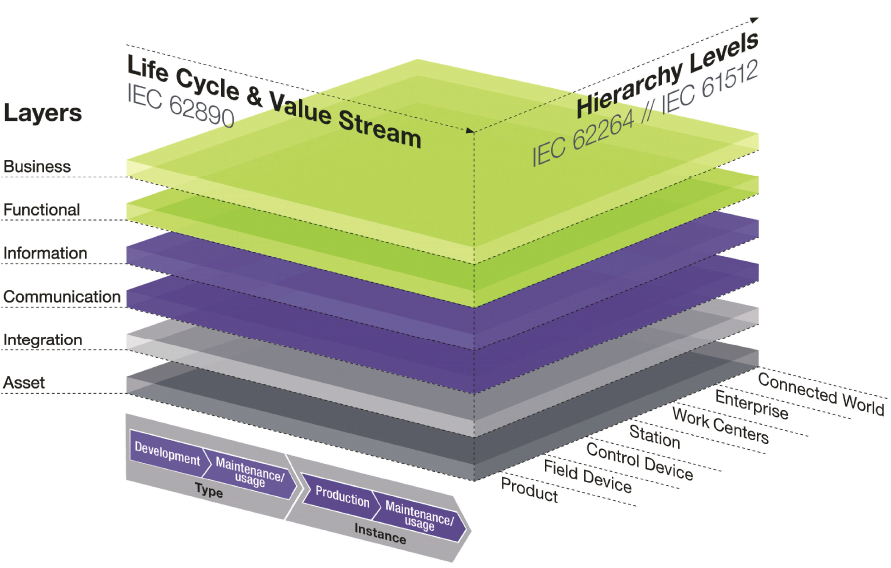
\includegraphics[width=0.8\textwidth]{Bilder/RAMI.PNG}
%     \caption{Referenzarchitekturmodell Industrie 4.0 (RAMI 4.0)}
%     \label{fig:klassifizierungDT}
% \end{figure}

\newpage
\subsection{Digitaler Zwilling}
\label{sec: DT}
Digitale Zwillinge gelten als eine der Schlüsseltechnologien der Industrie 4.0.
Als digitales Gegenstück eines physischen Objekts, sei es eine Maschine ein Produkt oder eine komplette Anlage, bilden sie dessen Zustand, Verhalten und Leistung virtuell ab.
Dadurch ermöglichen sie eine konsistenete Erfassung von Daten, das Simulieren von Prozessen und das frühzeitige Erkennen von Optimierungspotenzialen.

Das Konzept selbst wurde erstmals von Michael Grieves im Jahr 2003 in einer Präsentation zum \ac{plm} vorgestellt. 
Grieves definierte drei grundlegende Komponenten \cite{DTGrieves} , die zusammen das Informationsmodell des digitalen Zwilling bilden:
\begin{itemize}
    \item ein reales Objekt in der physischen Welt,
    \item ein digitales Abbild dieses Objekts in einem virtuellen Raum, sowie
    \item eine Schnittstelle, die den Informationsfluss zwischen diesen beiden ermöglicht.
\end{itemize}

Auf Basis des von Grieves entwickelten Informationsmodells hat sich der Begriff des digitalen Zwillings kontinuierlich weiterentwickelt.
Aufgrund verschiedener Fachgebiete und inkonsistenter Definitionen haben sich in der Vergangenheit allerdings eine Vielzahl unterschiedlicher Ausprägungen des Begriffs gebildet.
Diese unterscheiden sich insbesondere in der Tiefe der Datenintegration zwischen dem physischen Objekt und seinem virtuellen Abbild.
Während ein einfacher digitaler Zwilling lediglich ein einfaches Modell mit statischen Daten ist, ermöglichen fortgeschrittene Zwillinge einen bidrektionalen Datenaustausch zwischen physischem und virtuellem Objekt. 

Für ein besseres Verständnis und zur tieferen Klassifizierung ist es zunächst hilfreich, zwischen Typen und Instanzen des digitalen Zwillings zu unterscheiden.
Typen sind allgemeine Abbilder, die grundlegende Eigenschaften und Verhaltensmodelle einer Produktgruppe beschreiben. 
Sie können mit einer Klasse in der Softwarentwicklung verglichen werden, die als Vorlage für konkrete Instanzen dienen.
Typen können beispielsweise einen bestimmten Maschinentyp hinsichtlich Aufbau, Stuktur oder Schnittstellen beschreiben, ohne dabei Bezug zu einer einzelnen physischen Maschine zu nehmen.
Instanzen wiederrum sind einzigartig, und beschreiben ein konkretes Produkt, etwa eine Maschine, die einzigartig über eine Seriennummer identifizierbar ist.
Häufig sind Instanzen Aussprägungen eines Types mit einer Verbindung zu einem realen Objekt, wodurch beispielsweise die Überwachung des Zustands einer Produktionsanlage ermöglicht wird.
Analog zur Softwarentwicklung können diese als instanziiertes Objekt einer Klasse gesehen werden. \cite{ZEISS}

Je nach Art des Informationsflusses sowie dem Grad der Ausprägung der Verbindung zur realen Welt werden Instanzen digitaler Zwillinge häufig in drei Kategorien eingeteilt: das digitale Modell, den digitalen Schatten und den digitalen Zwilling \cite{ClassificationDT}.
Obwohl diese Begriffe im allgemeinen Sprachgebrauch oft synonym verwendet werden, unterscheiden sie sich deutlich hinsichtlich ihrer Funktion und Kopplung zum realen Objekt.

Digitale Modelle sind statische Abbilder physischer Objekte, haben jedoch keine Verbindung zu diesen. 
Oft werden sie zur Veranschauclichung oder Konstruktion genutzt, wie zum Beispiel ein 3D-Modell einer Maschine.
Zwar können reale Daten, wie etwa Maße oder Materialeigenschaften einer Anlage oder Maschine in ein solches Modell integriert werden, allerdings erfolgt die Eingabe dabei immmer manuell.
Änderungen an dem realen Objekt werden nicht automatisch aktualisiert und bleiben somit ohne Einfluss auf das digitale Modell.

Der digitale Schatten ergänzt das digitale Modell um eine unindirektionale Verbindung zum realen Objekt.
Dabei fließen Daten des physischen Objekts meist in Echtzeit über zum Beispiel geeignete Sensoren zum digitalen Objekt.
Der Schatten bildet den aktuellen Zustand des Objekts ab, hat aber keine Rückkoplung zu diesem.
Ein typisches Beispiel für einen digitalen Schatten wäre das Condition Monitoring, wobei der Zustand einer Maschine mit geeigneten Sensoren abgebildet wird.

Mit einer aktiven Rückkoplung zum realen Objekt wird der digitale Schatten zum digitalen Zwilling.
Es entsteht eine Feedback-Schleife, die es dem virtuellen Objekt erlaubt, Einfluss auf das reale System zu nehmen.
Eine Übersicht der drei Kategorien zeigt Abbildung \ref{fig:klassifizierungDT}. 
% Quelle: file:///C:/Users/Heinke/Documents/Bachelorarbeit/02%20Literatur/Digitaler_Zwilling/Klassifizierung_DT.pdf
\vspace{-0.5em}
\begin{figure}[htbp]
    \centering
    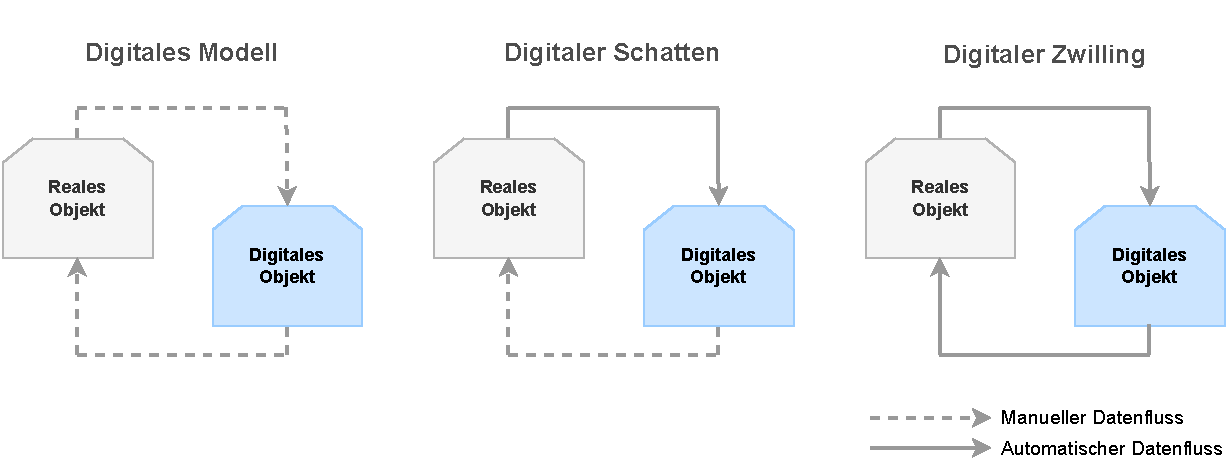
\includegraphics[width=1\textwidth]{Bilder/klassifizierung_DT.pdf}
    \caption[Klassifizierung des digitalen Zwillings]{Klassifizierung des digitalen Zwillings (in Anlehnung an \cite{ClassificationDT})}
    \label{fig:klassifizierungDT}
\end{figure}
\vspace{-0.5em}

Im industriellen Umfeld werden digitale Zwillinge in vielen unterschiedlichen Bereichen genutzt.
Sie kommen entlang des gesamten Lebenszyklus eines Assets zum Einsatz, von der Entwicklung über die Produktion bis hin zum Betrieb und der Wartung. 
\linebreak \newpage Dabei ist jedoch zu beachten, das in der Praxis häufig auch digital Modelle oder digitale Schatten als digitale Zwillinge bezeichnet werden, obwohl sie technisch gesehen nicht alle Merkmale eines echten digitalen Zwillings aufweisen und somit ebenfalls nicht ihr volles Potenzial entfalten.

Bereits bei der Entwicklung von Produkten können digitale Zwillinge einen erheblichen Vorteil bieten. 
Indem bereits frühzeitig digitale Modelle oder Simulationen eingesetzt werden, entfällt die Notwendigkeit physischer Prototypen, was Entwicklungszeiten und Kosten deutlich senken kann. Während der Produktion ermöglichen sie eine durchgängige Überwachung, Analyse und Optimierung von Fertigungsprozessen durch die Integration von Echtzeitdaten.
Sie unterstützen die virtuelle Inbetriebnahme von Maschinen und dienen als Grundlage für die vorausschauende Wartung (Predictive Maintenance), wodurch Stillstandzeiten einer Maschine reduziert werden können.
Nicht zuletzt dienen digitale Zwillinge als zentrale Datenplattform, in der alle relevanten Informationen aus verschiedenen Datenquellen gebündelt werden.
Sie bilden somit eine konsistente Datenbasis und können beispielsweise bei dem Entwicklungsprozess eines Produktes helfen. \cite{DTForSmartManufacturing}

Die Implementierung digitaler Zwillinge erweist sich in der Praxis jedoch oftmals als sehr anspruchsvoll.
Eine zentrale Herausforderung ist die fehlende Interoperabilität zwischen verschiedenen IT-Systemen.
Sowohl innerhalb eines Unternehmens als auch unternehmensübergreifend bilden sich dadurch häufig voneinander isolierte Datenbestände, die nicht systemübergreifend nutzbar sind.
Solche sogenannten Informationssilos können die Umsetzung eines konsistenten digitalen Zwillings erheblich erschweren, da die relevanten Informationen und Daten zunächst aus unterschiedlichen Systemen wie \ac{erp}, \ac{mes} oder \ac{cad} zusammengeführt werden müssen.

Hinzu kommt, das diese Daten oftmals in unterschiedlichen, nicht standardisierten Formaten vorliegen, was eine automatisierte Integration zusätzlich erschwert.
Diese Problematik zeigt sich nicht nur innerhalb einzelner Unterhnehmen, sondern auch entlang der gesamten Wertschöpfungskette, etwa wenn verschiedene Akteure einer Lieferkette heterogene Datenformate und proprietäre Austauschprotokolle verwenden.
Ein digitaler Zwilling, der in einem Unternehmen A erstellt wurde, kann dadurch von einer Anwendung oder einem weitern digitalen Zwilling eines Unternehmens B nicht ohne Weiteres intepretiert oder verwendet werden.
Es ist daher essenziell, digitale Zwillinge in einem interoperablen Format bereitzustellen, um eine einheitliche Interpretation und Nutzung auch über Unternehmensgrenzen hinweg zu ermöglichen.
\cite{DTandAASConceptsInI4.0}


% Definition nach Stark und Damerau des DT: 

% A digital twin is a digital representation of an active unique product (real device, object, machine, service, or intangible asset) or unique product-service system (a system consisting of a product and a related service) that comprises its selected characteristics, properties, conditions, and behaviors by means of models, information, and data within a single or even across multiple life cycle phases.

% \url{https://link.springer.com/referenceworkentry/10.1007/978-3-642-35950-7_16870-1#citeas}

\newpage
\subsection{Asset Administration Shell}
\label{chap:AAS}

% Das \ac{rami} ist ein Leitfaden für die Industrie und dient als Hilfestellung um die digitale Transformation in einem Unternehmen systematisch umzusetzten.
% Es wird in der DIN SPEC 91345 \cite{RAMI4.0} standardisiert und soll helfen, die komplexen Anforderungen an die Industrie 4.0 für die Allgemeinheit verständlich zu machen.
% Das Modell ist als dreidimensionales Koordinatensystem konzipiert und umfässt die Achsen ... .


Die \acs{aas} - deutsch Verwaltungsschale - ist eine Schlüsselkomponente innerhalb des \ac{rami} \cite{RAMI4.0} und bildet die Grundlage für die Umsetzung und Entwicklung interoperabler digitaler Zwillinge im industriellen Umfeld.
Sie wurde maßgeblich von der Plattform Industrie 4.0 entwickelt und erstmals im Jahr 2016 als Teil von \acs{rami} vorgestellt.
Seit ihrer Einführung wurde die \acs{aas} kontinuierlich weiterentwickelt und ist mittlerweile in der internationalen Norm IEC 63278-1 \cite{AASIEC63278} standardisiert.
% Darin wird die AAS als "strukturierte, standardisierte digitale Repräsentation eines Assets" definiert.

Seit 2020 wird die Umsetzung und Weiterentwicklung der \acs{aas} von der \acs{idta} \cite{IDTA} organisiert und gesteuert.
Ziel der Organisation ist es, den digitalen Zwilling auf Basis der \acs{aas} zu standardisieren und in Form von Open-Source-Softwarelösungen in das industrielle Umfeld zu integrieren.
Die \acs{aas} wird dabei in mehreren Spezifikationen der \acs{idta} dokumentiert und beschrieben.
Aktuell bildet die \acs{aas}-Version 3 den neuesten Entwicklungsstand und ist ebenfalls die Basis für diese Arbeit.
% evtl die Quelle wenn gut https://www.zvei.org/themen/start-der-industrial-digital-twin-association-idta

Die \acs{aas} repräsentiert ein Asset digital, indem sie alle relevanten Daten, Eigenschaften und Funktionen über den gesamten Lebenszyklus hinweg in strukturierter und standardisierter Form bereitstellt. 
Sie fungiert somit als digitales Gegenstück eines realen Objekts - also als digitaler Zwilling.
Die Informationen sind in sogenannten Submodellen organisiert, die jeweils spezifische Aspekte eines Assets abbilden.
Dabei kann es sich sowohl um physische Assets (z.B. Maschinen, Anlagen) als auch um virtuelle Assets (z.B. Software, Konzepte) handeln. 
Eine \acs{aas} ist dabei stets einem Asset zugeordnet und global eindeutig identifizierbar. 
Durch die Kombination eines Assets mit seiner \acs{aas} entsteht eine sogenannte Industrie 4.0-Komponente (siehe Abbildung \ref{fig:Industrie4Komponente}).

% Durch die standardisierte Struktur bildet die Verwaltungsschale die Grundlage für einen einheitlichen Informationsaustausch über System -und Unternehmensgrenzen hinweg.
% Verwaltungsschalen repräsentieren immer genau ein Asset und müssen global eindeutig identifizierbar sein.
% In der Industrie können Assets physische Objekte, wie eine Anlage oder eine Maschine sein oder aber auch virtuelle Elemente wie Software oder eine Idee.
% In RAMI 4.0 wird davon ausgegangen, das Assets immmer einen konkreten Nutzen für ein Unternehmen bzw. eine Organisation bieten.
\vspace{1em}
\begin{figure}[htbp]
    \centering
    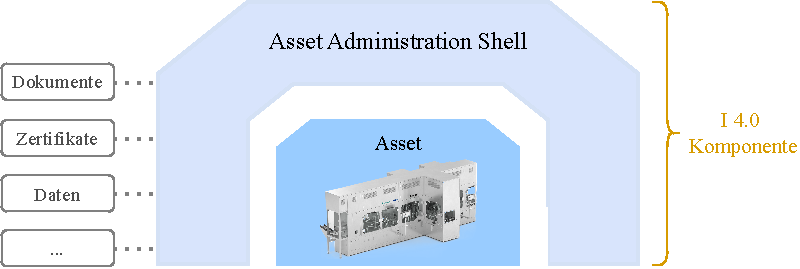
\includegraphics[width=1\textwidth]{Bilder/I4Komponente/I4KomponenteNeu.pdf}
    \caption[Industrie 4.0 Komponente]{Industrie 4.0 Komponente (Bildbestandteil: \cite{robocellLogo})}
    \label{fig:Industrie4Komponente}
\end{figure}

\subsubsection{Aufbau und Struktur}
Analog zur in Kapitel \ref{sec: DT} beschriebenen Unterscheidung von Typen und Instanzen digitaler Zwillinge unterscheidet auch die \acs{aas} zwischen diesen beiden Ausprägungen.
Während Typ-\acs{aas} allgemeine Merkmale und Strukturen eines Produkttyps beschreiben, sind Instanz-\acs{aas} konkreten physischen oder virtuellen Objekten zugeordnet und enthalten spezifische Informationen wie Seriennummer, Zustand oder Standort.

Bestimmte Aspekte eines Assets werden gemäß der Spezifikation des Metamodells der AAS \cite{SpezifikationPart1} in verschiedenen Submodellen verwaltet.
Man kann sich dies wie ein Schubladensystem vorstellen, wobei jede Schublade einen bestimmten Bereich des Assets abdeckt, beispielsweise die technischen Stammdaten, das Typenschild, Wartungsinformationen oder Zustandswerte einer Maschine.
Die Auswahl und Struktur der Submodelle ist domänenspezifisch und hängt stark vom konkreten Asset bzw. Anwendungsfall ab. 
Dabei kann eine \acs{aas} beliebig viele Submodelle enthalten, die bei Bedarf auch erweitert werden können. 

Die Daten innerhalb eines Submodells werden in verschiedenen Submodellelementen strukturiert.
Diese umfassen Dateneigenschaften, Operationen sowie weitere Sutrukturellemente die für eine umfassende Beschreibung eines digitalen Modells eines Assets erforderlich sind.
So erlaubt beispielsweise das RelationshipElement die Modellierung von Beziehungen oder das ReferenceElement die Referenzierung von internen oder externen Inhalten.
Das vermutlich am häufigsten verwendete Datenelement ist das Submodellelement Property.
Es lässt sich mit einer Variablen aus der Softwareentwicklung vergleichen, da es einfache Merkmale wie etwa einen Namen oder eine Seriennummer repräsentiert und dabei über einen definierten Datentyp wie String, Integer oder Boolean verfügt.

Wichtig ist, sowohl die \acs{aas} selbst als auch ihre Submodelle müssen global eindeutig identifizierbar sein.
Dies wird durch die Verwendung von eindeutigen Identifikatoren der Klasse Identifiable wie einer URI (Uniform Resource Identifier) oder \acs{irdi} (International Registration Data Identifier) sichergestellt.
Für die Elemente innerhalb eines Submodells ist eine lokale Kennung ausreichend. 
Dies erfolgt in der Regel anhand einer idShort der Klasse Referable, die einen kurzen, aussagekräftigen Namen enthält.

Zur besseren Veranschaulichung der zugrunde liegenden Struktur der \acs{aas} dient Abbildung \ref{fig:MetamodellAAS}, die eine vereinfachte Darstellung des Metamodells zeigt.

% Neben Properties spielt zudem das Submodellement File eine besonders wichtige Rolle. Es ermöglicht das Einbetten oder Referenzieren von Dateien in die \acs{aas}. 
% Dabei werden gängige Dateiformate wie PDF, JPG oder STEP unterstützt, was besonders für technische Dokumentationen oder \acs{cad}-Modelle von Bedeutung ist.
% Neben diesen Datenelementen existieren noch weitere Submodellelemente, die spezifische Funktionen ermöglichen. 
% So erlaubt beispielsweise das RelationshipElement die Modellierung von Beziehungen oder das ReferenceElement die Referenzierung von internen oder externen Inhalten.
% Zur besseren Veraunschaulichung des zugrundeliegenden Metamodells wird dieses nachfolgend in einer vereinfachten Form dargestellt.

\newpage
\begin{figure}[htbp]
    \centering
    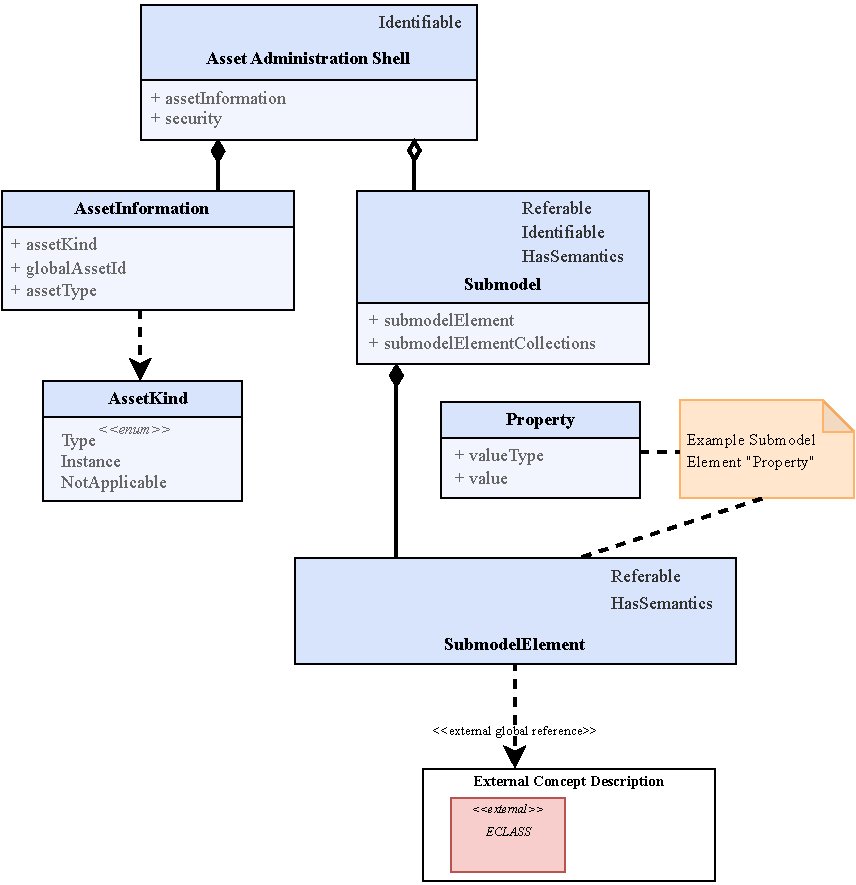
\includegraphics[width=1\textwidth]{Bilder/Metamodell/MetamodellFarbig.pdf}
    \caption[Vereinfachtes Metamodell der \acs{aas}]{Vereinfachtes Metamodell der \acs{aas} (in Anlehnung an \cite{SpezifikationPart1})}
    \label{fig:MetamodellAAS}
\end{figure}

Eine eindeutige semantische Beschreibung aller Submodelle und ihrer Elemente ist essenziell, um ein einheitliches Verständnis zwischen unterschiedlichen Systemen sicherzustellen.
Hierfür wird die sogenannte semanticID der Klasse HasSemantics verwendet, welche eine semantische Referenz enthält.
Diese verweist entweder auf einen externen Standard oder auf eine lokale \ac{cd}, die direkt in der \acs{aas} eingebettet ist.
Ein häufig verwendeter externer Standard ist zum Beispiel ECLASS, welcher auf der Norm IEC 61360 \cite{ECLASSIEC61360} basiert.

Zur formalen Beschreibung solcher Concept Descriptions stellt die \acs{idta} standardisierte Data Specification Templates gemäß der Norm IEC 6130 \cite{SpezifikationPart3a} bereit.
Diese liefern ein strukturiertes Modell zur Beschreibung technischer Merkmale.
Darin enthalten sind unter anderem Definitionen, Einheiten, Wertebereiche, zulässige Werte sowie externe Referenzen, die bestimmten Submodellen oder Submodellelementen zugeordnet werden können.
% Dadurch wird ein gemeinsames semantisches Verständnis zwischen unterschiedlichen Systemen ermöglicht.

%Fehlt die semantische Beschreibung, so kann es schnell zu Missverständnissen kommen.
%Liegt beispielsweise ein einfacher Wert 25 vor, ist ohne weitere Informationen unklar, was gemeint ist. 
%Es könnte sich um 25 Euro, 25 Meter oder 25 Grad Celsius handeln.
%Erst durch die zugehörige semantische Beschreibung, in der die Einheit und Bedeutung definiert werden, wird der Wert eindeutig interpretierbar. 

Um die Erstellung von Submodellen zu erleichtern und gleichzeitig Interoperabilität zu gewährleisten, stellt die \acs{idta} standardisierte Submodellvorlagen - sogenannte \acp{smt} - zur Verfügung.
Diese Templates decken eine Vielzahl industrieller Anwendungsfälle ab und werden kontinuierlich weiterentwickelt und ergänzt.
Die bereits verfügbaren Templates enthalten unteranderem Submodelle wie das digitale Typenschild oder den \ac{cf}.
Alle Eigenschaften innerhalb dieser Vorlagen werden dabei in Verbindung mit dem ECLASS-Standard einheiltich semantisch beschrieben.
Diese Templates könen über ein zentrales Repository \cite{idtaTemplates} bezogen werden und bilden die Basis für eine interoperable semantische Datenstruktur.

\subsubsection{Informationsaustausch}
Der Austausch von Informationen über die \acs{aas} kann auf unterschiedliche Weise erfolgen.
Die einfachste Möglichkeit besteht im Dateiaustausch. Hierfür wurden speziell für die \acs{aas} sogenannte AASX-Dateien \cite{SpezifikationPart5} entwickelt, die den einfachen Austausch statischer \acs{aas} (Typ-1-\acs{aas}) ermöglichen.
Dabei werden sämtliche Daten, Beziehungen, Strukturen sowie zugehörige Dateien der \acs{aas} serialisiert und in ein AASX-ZIP-Dateiformat gespeichert. 
Diese Datei kann anschließend über ein digitales Medium, etwa per E-Mail oder eine Cloud-Plattform, weitergegeben werden. 

Eine Typ-2-\acs{aas} hingegen wird von einer Laufzeitumgebung gehosted, wodurch ein direkter und dynamischer Zugriff auf ihre Inhalte ermöglicht wird. 
Die Spezifikitation Part 2: Aplication Programming Interfaces \cite{SpezifikationPart2} beschreibt hierfür nicht nur standardisierte Schnittstellen, sonder auch ein ganzheitliches System für das Verwalten, Bereitstellen und Auffinden der \acs{aas}.
Repositories dienen dabei als zentraler Speicherort für die Inhalte einer \acs{aas}, einschließlich ihrer Submodelle und Concept Descriptions.
Die Aufgabe der Verwaltung und Registrierung übernehmen sogenannte Registries.
Sie ermöglichen das systemweite Auffinden von \acs{aas} und stellen sicher, dass diese eindeutig referenzierbar sind.

Ergänzend dazu bieten Discovery Services eine erweiterte Suchfunktionalität, indem sie Beziehungen verschiedener Entitäten mittels verschiedener Schlüsselwertpaare speichern.
Eine \acs{aas} kann so zum Beispiel logisch mit einer \acs{assetid} (Asset Identifier) verknüpft werden und somit schnell innerhalb komplexer Systeme identifiziert werden.
Der Zugriff auf diese Systeme bzw. ihrer Inhalte wird in Form von Schnittstellen standardisiert, wodurch eine hohe Interoperabilität gewährleistet wird.
Ein besonderer Fokus liegt dabei auf der Nutzung von \ac{http} gemäß dem \acs{rest}-Architekturstil (Representational State Transfer), der eine strukturierte Kommunikation über Methoden wie GET, POST, PUT oder DELETE ermöglicht.

Die fortschrittlichste Form des Informationsaustausches stellt die Peer-to-peer Kommunikation dar, bei der I4.0-Komponenten (Typ-3-\acs{aas}) eigenständig über die I4.0-Sprache miteinander kommunizieren.

\subsubsection{Sicherheit}
\label{sec: Sicherheit}
Gerade wenn Informationen aus der \acs{aas} über die Grenzen des eigenen Unternehmens hinweg bereitgestellt werden, ist es besonders wichtig, dass die enthaltenen Daten geschützt sind. 
Die neueste Spezifikation Part 4: Security \cite{SpezifikationPart4} der \acs{idta} liefert hierfür die technische und konzeptionelle Grundlage.
Sie beschreibt, wie Zugriffe auf Daten in der \acs{aas} sicher gesteuert werden können, insbesondere in vernetzten Umgebungen wie Datenräumen.

Zum Einsatz kommen dabei Dienste wie ein Identity Provider zur Authentifizierung oder ein Policy Service zur Durchsetzung von Richtlinien.
Die Sicherheit wird dabei mithilfe eines attributbasierten Zugriffsmodells (\ac{abac}) gewährleistet.
Bei jeder Anfrage auf bestimmte Objekte innerhalb der \acs{aas} wird dabei anhand verschiedener Merkmale (Attribute) geprüft, ob ein Zugriff erlaubt ist.
Dazu zählen sogenannte Subjektattribute (also wer die Anfrage stellt), Objektattribute (z.B. welches Submodell, welche Property oder welches Submodellelement betroffen ist), die gewünschte Aktion (z.B. Lesen oder Schreiben) sowie kontextbezogene Bedingungen (z.B. Zeitpunkt der Anfrage oder Zustand des Systems).

Die zur Prüfung notwendigen Informationen liefert in der Regel ein Token, das vom Identity Provider bereitgestellt wird. Die Spezifikation sieht hierfür die Nutzung sogenannter \acp{jwt} vor.
Die Attribute werden schließlich von dem Policy Service mit den dort hinterlegenen Zugriffsrichtlinen abgeglichen und basierend darauf eine Zugriffsentscheidung getroffen.
Ein besonderer Vorteil des \acs{abac}-Modells liegt dabei in seiner hohen Flexibilität. Rollen können ebenfalls als Attribute behandelt werden, wodurch sich auch problemlos rollenbasierte Zugriffskonzepte (RBAC) umsetzen lassen. 

Die beschriebenen Kontrollmechanismen lassen sich nicht nur auf die Inhalte der \acs{aas} selbst, sondern insbesondere auch auf die Schnittstellen von Registries und Repositories anwenden.
So kann beispielsweise sichergestellt werden, das nur authorisierte Systeme Zugriff auf ein bestimmtes Submodell erhalten oder nur bestimmte Nutzergruppen neue \acs{aas}-Instanzen registrieren können.
Diese Sicherheits-Konzepte sind jedoch noch \linebreak \newpage vergleichsweise neu und müssen in der Praxis erst noch weiter erprobt werden.
Erste Referenzimplementierungen liegen zwar bereits häufig schon in Form rollenbasierter Zugriffskontrollen vor, eine vollständige Integration des \acs{abac}-Ansatzes steht jedoch noch aus.


\subsection{Digitaler Produktpass}
Der \acs{dpp} ist ein zentrales Instrument der Europäischen Union zur Umsetzung einer nachhaltigen, digitalen Transformation. 
Ziel ist es, die Transparenz über ökologische Merkmale von Produkten wie verwendete Materialien, Recylcebarkeit oder die CO\textsubscript{2}-Bilanz deutlich zu verbessern.
Hierzu müssen produktspezifische Daten über den gesamten Lebenszyklus hinweg aufgezeichnet und in einem menschen -und maschinenlesbarem Format bereitgestellt werden. \cite{DPPEinführung}
Langfristig soll dies zu einer Kreislaufwirtschaft und digitalen Wirtschaft innerhalb der EU führen.

Das Konzept des \acs{dpp} wurde erstmals im Rahmen des European Green Deal von der Europäischen Kommission im Jahr 2019 vorgestellt \cite{GreenDeal}.
Im Zuge der Ökodesign-Verordnung (\ac{espr}) \cite{ESPR} wird er aktuell als verpflichtendes Mittel für zahlreiche Produktgruppen eingeführt.
Als erste konkrete Anwendung wird der \acs{dpp} erstmals im Jahr 2027 für Batterien verpflichtend.
Weitere Produktkategorien, darunter auch die Elektroindustrie und der Maschinen -und Anlagenbau werden in den nächsten Jahren folgen.

Die Bereitstellung der Produktpässe erfolgt gemäß den Anforderungen der \acs{espr} in elektronischer Form. 
Dabei müssen diese untereinander interoperabel kommunizieren können.
Je nach Art der Information werden verschiedene Zugriffsrechte für unterschiedliche Interessengruppen eingeführt. 
Damit soll der Schutz von geistigem Eigentum sichergestellt werden.
Die Daten sollen dabei über einen zentralen Server bzw. ein Registry verwaltet werden, worin die verschiedenen \acsp{dpp} gespeichert bzw. registriert werden.
\cite{CIRPASS}

Während die regulatorischen Rahmenbedingungen mehr oder weniger final ausgearbeitet sind, bleibt die Frage der konkreten technologischen Umsetzung.
Eine dezentrale Lösung bildet der von der \acs{zvei} vorgestellte digitale Produktpass für Industrie 4.0 (\acs{dpp40}) \cite{DPP40}.
Dieser basiert auf zwei etablierten Standards. 
Zum Einen das digitale Typenschild, und zum Anderen die \acs{aas} (siehe auch Kapitel~\nameref{chap:AAS}).
Das digitale Typenschild ermöglicht, gemäß der Norm IEC 61406 \cite{TypenschildIEC61406-1}, die eindeutige Identifikation von Produkten über eine einzigartige \acs{assetid}.
Typischerweise wird diese in Form eines maschinenlesbarem Links oder QR-Codes an einem Produkt angebracht, die direkt zu dem zugehörigen \acs{dpp} führt.

Organisiert werden die Daten im \acs{dpp40} in verschiedenen Submodellen der \acs{aas}. 
Standardisierte Teilmodelle wie das digitale Typenschild, Dokumentationen oder der \ac{pcf} helfen bei der Umsetzung der im \acs{dpp} geforderten Daten.
Darüber hinaus können auch zusätzliche, nicht verpflichtende Informationen integriert werden, sofern sie für bestimmte Stakeholder einen Mehrwert bieten.
Der Zugriff auf die Daten ist über ein webbasiertes Portal vorgesehen. 

Verschiedene Interessengruppen erhalten dabei unterschiedliche Zugriffsrechte. 
Hierfür werden bestimmmte Submodelle gezielt für unterschiedliche Gruppen freigegeben oder eingeschränkt.
Während beispielsweise das Typenschild oder der \acs{pcf} öffentlich zugänglich sind, werden sensible Informationen wie technische Dokumentationen oder sicherheitsrelevante Details nur bestimmten autorisierten Gruppen zugänglich gemacht.

Das Konzept der \acs{zvei} sieht darüber hinaus vor, dass Unternehmen ihre \acsp{dpp} entgegen den Anforderungen der \acs{espr} dezentral in einem eigenen Repository verwalten. 
Diese können entweder vom produzierenden Unternehmen selbst oder von Dritten, etwa Cloud-Dienstleistern, im Auftrag betrieben werden. 
Ziel ist es, Unternehmen die Möglichkeit zu geben, ihre Daten bei Bedarf eigenständig zu aktualisieren und gleichzeitig die Kontrolle über sensible Informationen zu behalten.

Zur Koordination dieser dezentralen Systeme ist ein zentrales Registry vorgesehen, in der alle Repositories registriert werden.
Über dieses können interessierte Akteure relevante Server identifizieren und gezielt auf freigegebene Submodelle eines Produktpasses zugreifen.
So wird sichergestellt, dass trotz der dezentralen Struktur eine durchgängige Interoperabilität gewährleistet ist, wie sie für die Umsetzung des \acs{dpp} auf europäischer Ebene erforderlich ist.

\subsection{robocell}
Die robocell ist eine von groninger in Zusammenarbeit mit SKAN entwickelte Maschinenlinie zur aseptischen Abfüllung von genesteten Spritzen, Zylinderampulen und Vials.
Sie zeichnet sich dadurch aus, dass alle Prozesschritte vollständig automatisiert ablaufen.
Durch den gezielten Einsatz von Robotern kann der menschliche Eingriff auf ein Minimum reduziert werden, wodurch maximale Sicherheit, Flexibilität und Effizienz im Abfüllprozess gewährleistet wird \cite{RobocellWebsite}.

Die Linie besteht aus mehreren modular aufgebauten Einzelmaschinen, die jeweils spezifische Aufgaben entlang des Produktionsprozesses übernehmen. 
Im Rahmen dieser Arbeit liegt der Fokus auf dem in Abbildung~\ref{fig:robocell} gezeigten hochautomatisierten Abfüll- und \linebreak 
\newpage Verschließmodul, das für das vollautomatisierte Abfüllen und Verschließen von Behältnissen verantwortlich ist.

\begin{figure}[htbp]
    \centering
    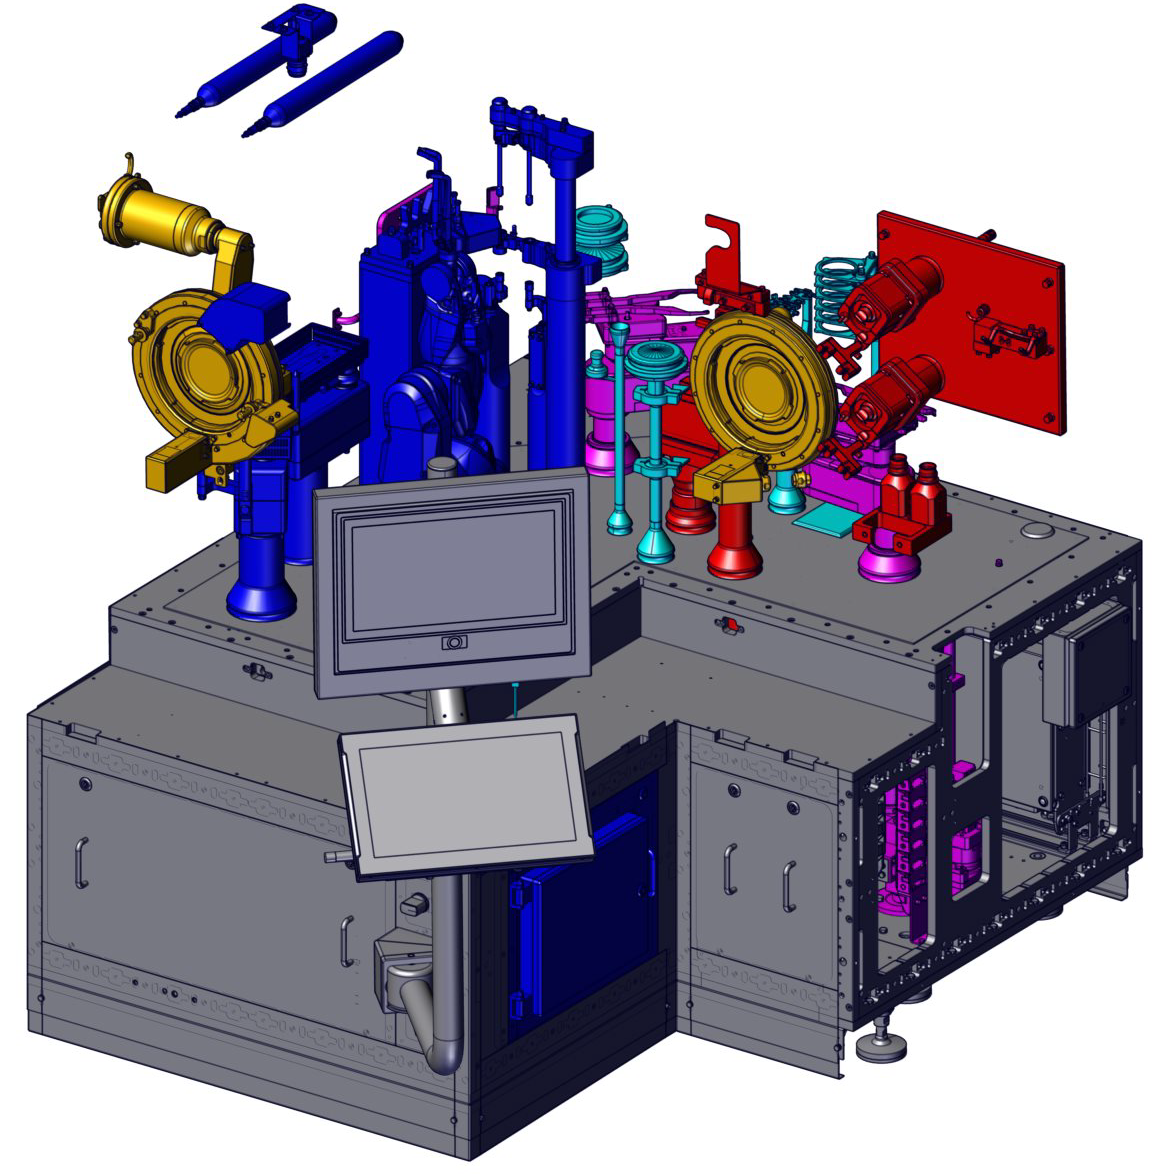
\includegraphics[width=0.5\textwidth]{Bilder/robocell/filling_closing_module.png}
    \caption[robocell Abfüll- und Verschließmodul]{robocell Abfüll- und Verschließmodul (Quelle: \cite{RobocellBetriebsanleitung})}
    \label{fig:robocell}
\end{figure}

\vspace{-0.25em}
\subsection{Technologische Grundlagen}
Im Folgenden werden die technologischen Grundlagen erläutert, die für das Verständnis und die Umsetzung dieser Arbeit besonders relevant sind.
\subsubsection{AASX Package Exlporer}
Der AASX Package Explorer, nachfolgend als Package Explorer bezeichnet, wurde als Referenzimplementierung für die \acs{aas} gemäß den Spezifikationen der \acs{idta} entwickelt.
Das Tool ist als Open-Source-Software \cite{AASXPackageExplorer} verfügbar und ermöglicht das Erstellen und Bearbeiten von \acs{aas} im standardisierten AASX-Dateiformat.

Der Package Explorer verfügt dabei über eine benutzerfreundliche grafische Oberfläche (siehe Abbildung \ref{fig:AASXPackageExplorer}), die insbesondere Einsteigern den Zugang zur Modellierung erleichtert.
Dabei können Submodelle, Eigenschaften, semantische Referenzen sowie Metadaten strukturiert definiert und verwaltet werden.
Gleichzeitig bietet der Package Explorer auch erweiterte Funktionen, wie das Erstellen von \acsp{smt}, wodurch er sich auch für den profesionellen Einsatz eignet.

Neben der lokalen Modellierung erlaubt das Tool ebenfalls die Verbindung zu einem AAS-Server über standardisierte Schnittstellen (z.B. \acs{opcua} oder \acs{http}/\acs{rest}).
Dies ermöglicht den Betrieb von \acs{aas} in verteiltelten Systemen.
Besonders geeignet hierfür \linebreak \newpage ist der Referenzserver des Eclipse-AAS-Projekts \cite{AASXServer}, der das Hosten und Bereitstellen von AASX-Paketen ermöglicht sowie eine nahtlose Integration mit dem Package Explorer erlaubt.

\begin{figure}[htbp]
    \centering
    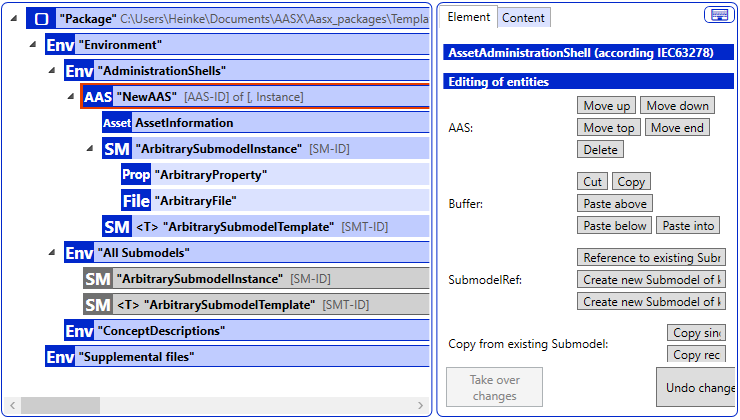
\includegraphics[scale=0.765]{Bilder/ModellierungAAS/Final/Grundlagen_PE.PNG}
    \caption[Benutzeroberfläche Package Explorer]{Benutzeroberfläche Package Explorer (eigene Darstellung)} 
    \label{fig:AASXPackageExplorer}
\end{figure}

\subsubsection{Eclipse BaSyx }
Eclipse BaSyx ist eine vom Fraunhofer-Institut für Experimentelles Software Engineering entwickelte Open-Source-Plattform für die Realisierung von Industrie-4.0-Anwendungen.
Mittlerweile wird das Projekt unter dem Dach der Eclipse Foundation weitergeführt.
Der Fokus liegt auf einer einfachen Umsetzung einer Infrastruktur zur Erstellung und Verwaltung digitaler Zwillinge auf Basis der \acs{aas}.
Die Software steht dabei allen Interessenten frei zur Verfügung.

Die Softwarearchitektur basiert auf einer Vielzahl von Standardkomponenten (Off-the-Shelf), die alle als Docker-Container frei zugänglich sind und somit eine nahtlose Integration in bestehende Docker-Umgebungen erlauben.
Eine der wichtigsten Komponenten ist die Registry. 
Sie ist, genau wie alle anderen Komponenten, auf den Spezifikationen der \acs{aas} aufgebaut, insbesondere auf der Spezifikation Part 2: Application Programming Interfaces \cite{SpezifikationPart2}.
In ihr können neue \acs{aas} registriert und bereits vorhandene \acs{aas} anhand ihrer eindeutigen Kennung gesucht werden.
Sie bildet damit die zentrale Anlaufstelle für Geräte und Anwendungen innerhalb des BaSyx-Systems.
Analog dazu existiert eine seperate Registry für die Verwaltung von Submodellen.

\newpage
Die eigentlichen Daten werden in der sogenannten \acs{aas} Environment gespeichert und organisiert.
Sie umfasst Repositories für \acs{aas}, Submodelle und Concept Descriptions.
In der Regel ist eine Datenbank, standardmäßig eine MongoDB als persistenter Speicher hinterlegt.
Wie auch alle anderen Komponente stellen diese Repositories standardisierte Schnittstellen basierend auf der \acs{api}-Spezifikation zur Verfügung.
Dies erlaubt z.~B. das Abfragen, Erstellen oder Aktualisieren einer \acs{aas} samt ihrer Submodelle und Inhalte.
Alle verfügbaren Endpunkte dieser Schnittstellen können unter anderem in der automatisch generierten Swagger-Dokumentation eingesehen und ausgeführt werden. 
Typische \acs{rest}-Endpunkte sind beispielsweise:

% \vspace{1em}
{\small
\begin{longtblr}[
  label = tab:aas_endpoints,
  caption = {REST-Endpunkte in Eclipse BaSyx},
  entry = REST-Endpunkte in Eclipse BaSyx
]{
  colspec = {c l X},
  rowhead = 1,
  vlines,
  hlines
}
\textbf{Methode} & \textbf{Endpunkt} & \textbf{Beschreibung} \\
\textcolor{green!50!black}{\textit{GET}} & \texttt{/shells} & Liste aller AAS abrufen \\
\textcolor{green!50!black}{\textit{GET}} & \texttt{/shells/\{aasIdentifier\}} & Bestimmte AAS anzeigen \\
\textcolor{green!50!black}{\textit{GET}} & \texttt{/submodels} & Liste aller Submodelle aufrufen \\
\textcolor{orange!85!black}{\textit{POST}} & \texttt{/shells} & Neue AAS erstellen \\
\textcolor{orange!85!black}{\textit{POST}} & \texttt{/submodels} & Neues Submodell erstellen \\
\textcolor{red!80!black}{\textit{DELETE}} & \texttt{/shells/\{aasIdentifier\}} & AAS löschen \\
\end{longtblr}
}
\vspace{-0.5em}

Im BaSyx-System ermöglicht ein Discovery Service die Verknüpfung physischer Assets mit iheren zugehörigen \acs{aas}.
% Dabei wird eine spezifische \acs{assetid} mit der entsprechenden AAS-ID verlinkt.
Dies ist insbesondere für die Abbildung von hierarchischen Strukturen wie Stücklisten (\ac{bom}) von großer Bedeutung.
Ein übergeordnetes Asset (z.B. Maschine) kann so beispielsweise mit untergeordneten Komponenten (z.B. Antrieb, Sensoren) logisch über deren AAS verbunden werden.
Einträge in den Discovery Service müssen derzeit allerdings noch manuell über die \acs{api} (Aplication Programming Interface) vorgenommen werden.

Zur benutzerfreundlichen Visualisierung und Interaktion kann die sogenannte AAS Web UI genutzt werden.
Die webbasierte Benutzeroberfläche, wie in Abbildung \ref{fig:BasyxWebUI} dargestellt ist, wurde mit dem JavaScript-Framework Vue.js entwickelt und kommuniziert über die standardisierte \acs{rest}-API mit den zentralen Komponenten der BaSyx-Plattform, darunter die Repositories, Registries und der Discovery Service.
Sie zeigt alle registrierten \acs{aas} in einer Liste an und bietet die Möglichkeit, einzelne \acs{aas} in einer Baumstruktur sowohl zu visualisieren als auch zu bearbeiten. 

Ein weiteres zentrales Merkmal der AAS Web UI ist der sogenannte AAS Viewer.
In nachfolgender Abbildung ist dieser auf der rechten Seite angeordnet.
Er erlaubt die Visualisierung von Submodellen und deren Elementen anhand ihrer semanticID. 
Hierfür stehen verschiedene vordefinierte Plugins zur Verfügung, die bestimmte Submodelle, wie beispielsweise das Typenschild oder hierarchische Strukturen, grafisch darstellen.
Da die Lösung Open Source ist besteht zudem die Möglichkeit, eigene benutzerdefinierte Plugins für weitere Submodelle zu erstellen. \cite{BaSyxWiki} \cite{BaSyxEclipse}

\vspace{0.5em}
\begin{figure}[htbp]
    \centering
    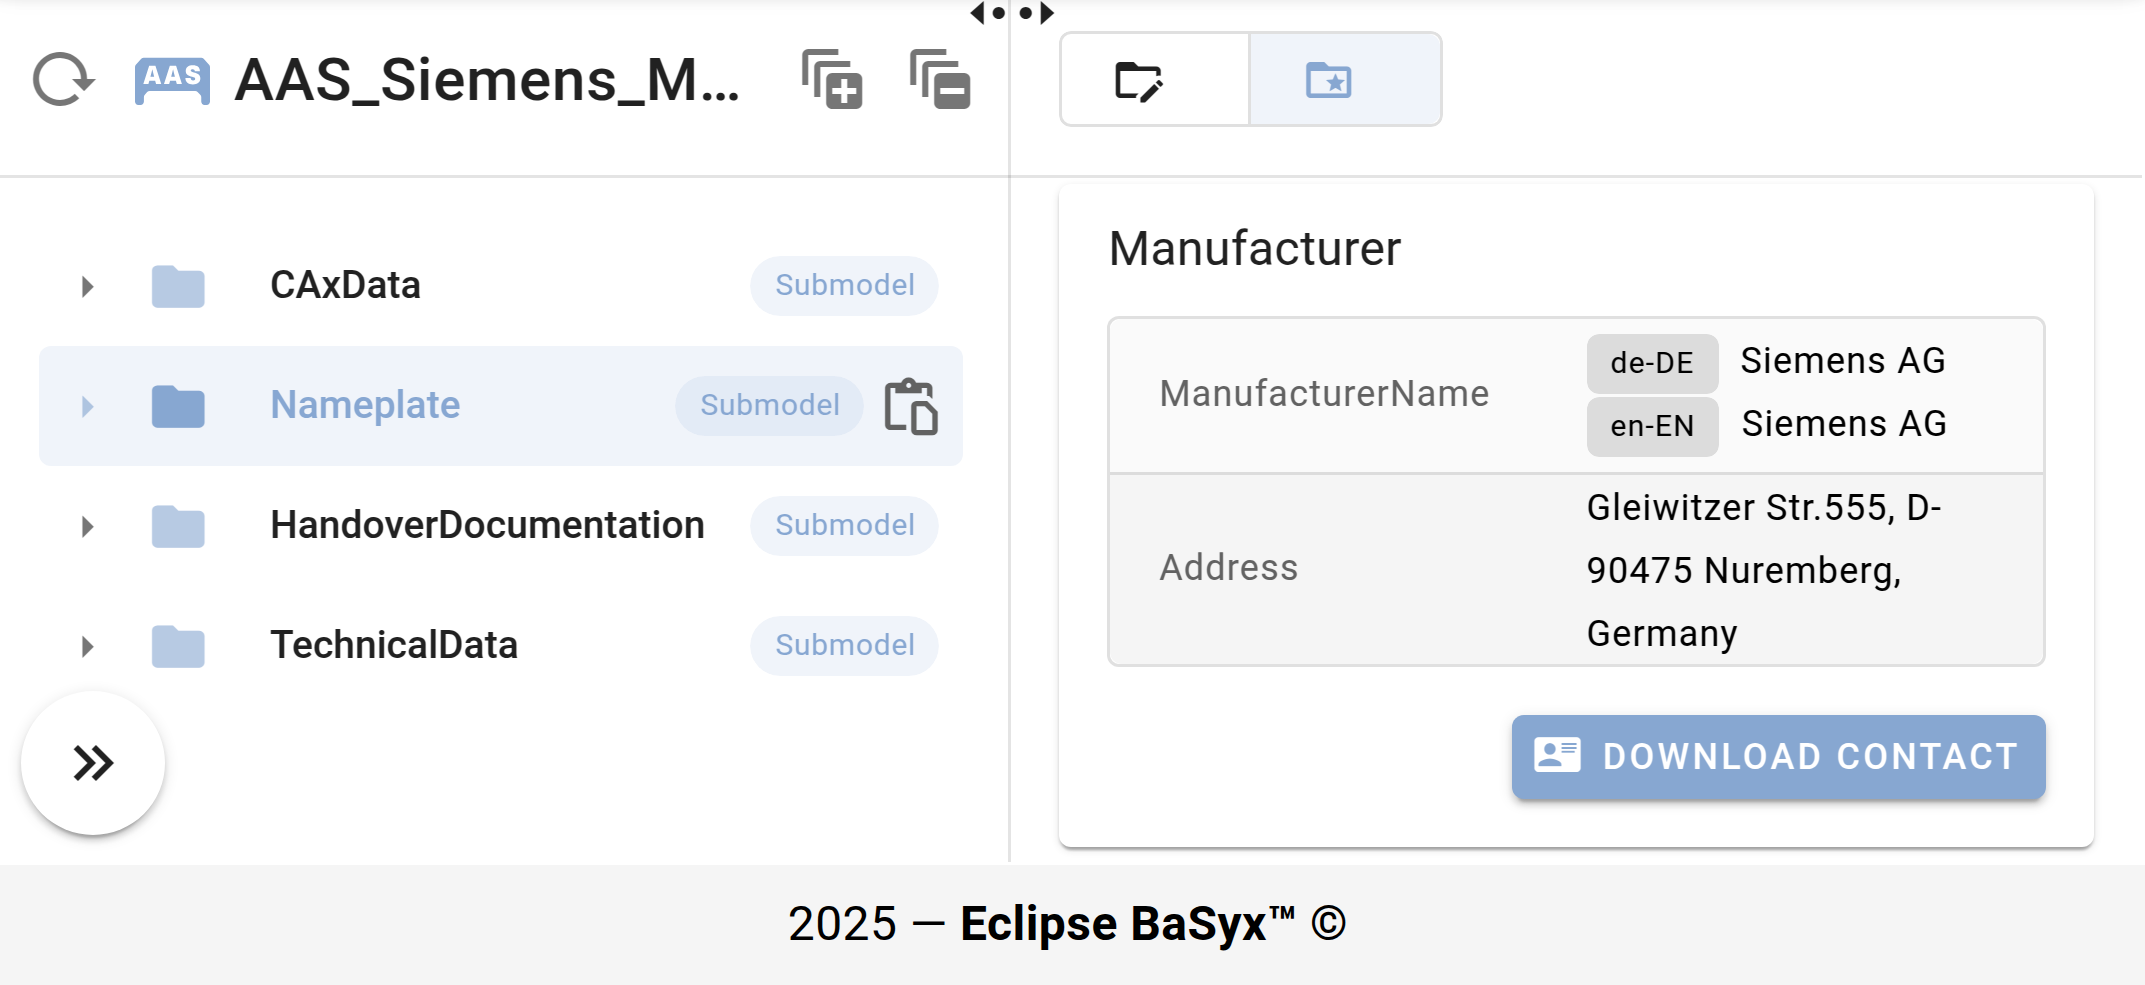
\includegraphics[width=1\textwidth]{Bilder/AASWebUZIGrundlagen.png}
    \caption[Benutzeroberfläche AAS Web UI]{Benutzeroberfläche AAS Web UI (eigene Darstellung)}
    \label{fig:BasyxWebUI}
\end{figure}


\subsubsection{OPC Unified Architecture}
\acs{opcua} ist ein plattformübergreifender Kommunikationsstandard, der speziell für die Anforderungen der industriellen Automatisierung entwickelt wurde.
Ziel ist ein herstellerübergreifender, sicherer und standardisierter Datenaustausch.
In \acs{rami} \cite{RAMI4.0} wird \acs{opcua} als empfohlener Standard für die Kommunikationsschicht definiert und bildet damit die Grundlage für die Interoperabilität zwischen Maschinen, Anlagen und IT-Systemen verschiedener Hersteller.

Die grundlegende Idee von \acs{opcua} besteht darin, dass ein Maschinenhersteller einen \acs{opcua} Server bereitstellt, der einen standardisierten und herstellerunabhängigen Zugriff auf eine Maschine ermöglicht.
Der Server dient hierbei als zentrale Schnittstelle zur Außenwelt. Er implementiert den OPC Standard und stellt strukturierte Informationen sowie Zugriffsmöglichkeiten auf Maschinenzustände und -daten bereit.
Im Inneren kommuniziert der Server dabei über ein herstellerspezifisches, proprietäres Protokoll mit der Steuerung.
Zum Auslesen oder Austauschen dieser Daten wird ein \acs{opcua} Client benötigt. Dieser agiert als Kommunikationspartner des Servers, stellt die Verbindung her und ermöglicht den bidirektionalen Datentransfer. \cite{OPCUA}
\newpage
\section{Entwicklung}
In diesem Kapitel wird die schrittweise Entwicklung des digitalen Zwillings für das Abfüll- und Verschließmodul der robocell-Linie dargestellt.
Ziel ist es, das physische Asset gemäß dem Konzept der \acs{aas} digital abzubilden und in ein Industrie 4.0-konformes System zu integrieren.
Abbildung \ref{fig:Entwicklungsschritte} veranschaulicht den Ablauf des zugrundeliegenden Entwicklungsprozesses.

\begin{figure}[htbp]
    \centering
    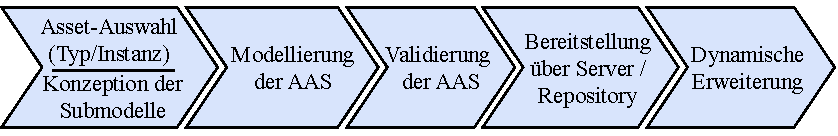
\includegraphics[width=1\textwidth]{Bilder/vorgehenEntwicklungsteil.pdf}
    \caption{Meine Bildunterschrift!!!!!}
    \label{fig:Entwicklungsschritte}
\end{figure}
\vspace{-1em}

Aufbauend auf einer konzeptionellen Grundlage erfolgt zunächst die statische Modellierung der \acs{aas} mithilfe des Package Explorers. 
Die resultierende Struktur wird anschließend mit einer Test Engine validiert.
Im weiteren Verlauf wird die \acs{aas} mit der Eclipse BaSyx-Plattform bereitgestellt und um dynamische Informationen ergänzt. 
Dabei werden sowohl Echtzeitdaten über \acs{opcua} als auch Zeitreihendaten über eine InfluxDB eingebunden.

Abschließend wird die Entwicklung von drei exemplarischen Anwendungsfällen betrachtet. 
Dazu zählen die Umsetzung eines digitalen Produktpasses, die automatisierte Generierung und Bereitstellung von \acs{aas}-Instanzen sowie der Einsatz von \acs{ki} im Kontext des digitalen Zwillings.

\subsection{Konzeptionierung des digitalen Zwilling}
Ziel dieses Abschnittes ist es, eine grundlegende Basis für die Erstellung des digitalen Zwillings zu schaffen.
Dabei wird untersucht, welche Daten für die Modellierung erforderlich sind, wo diese herkommen und wie sie in (standardisierten) Submodellen der \acs{aas} strukturiert werden können.
\subsubsection{Identifikation relevanter Datenquellen}
Ein digitaler Zwilling basiert immmer auf einer Vielzahl unterschiedlicher Daten, die gemeinsam ein umfassendes digitales Abbild eines Assets ermöglichen. 
Dabei werden sowohl statische Informationen (z.B. Datenblätter oder Konstruktionsdaten) als auch dynamische Daten, die während des Betriebs einer Maschine anfallen, benötigt.
Im ersten Schritt gilt es daher, alle relevanten Datenquellen zu identifizieren, die für die Modellierung des digitalen Zwillings erforderlich sind.

In industriellen Umgebungen kommen typischerweise verschiedene Systeme zur Erfassung, Verwaltung und Speicherung von Maschinendaten zum Einsatz.
Bei groninger übernimmt diese Funktion das \acs{plm}-System Agile, das eng mit dem \acs{erp}-System PSI Penta verknüpft ist.
Darin sind unter anderem Stücklisten, technische Spezifikationen, \acs{cad}-Dateien sowie allgemeine Dokumente hinterlegt, die die statische Grundlage  für den digitalen Zwilling bilden.

Neben den Informationen aus den Unternehmenssystemen spielen aber auch Laufzeitdaten, wie sie durch Sensoren oder Steuerungssysteme erzeugt werden, eine zentrale Rolle.
Da im Rahmen dieser Arbeit keine reale Maschine angebunden ist, werden diese Daten simuliert.
Hierfür kommt eine in Node.js entwickelte Anwendung zum Einsatz, die im Folgenden als Datengenerator bezeichnet wird und sowohl Prozess- als auch Betriebsdaten generiert. 
Ergänzend dazu wird ein Maschinensimulator verwendet, der einen PackML-Zustandsautomaten abbildet und typische Maschinenzustände sowie deren Übergänge simuliert. 
Beide Komponenten stehen als Docker Container zur Verfügung und stellen die Daten über einen \acs{opcua} Server bereit, wodurch eine realitätsnahe Datenbasis geschaffen wird.
\subsubsection{Auswahl geeigneter Teilmodelle}
Aufbauend auf den zuvor betrachteten Informationsquellen gilt es nun zu entscheiden, welche Aspekte der Maschine im digitalen Zwilling, oder besser gesagt in der \acs{aas}, abgebildet werden sollen.
Im nächsten Schritt ist daher die Auswahl bzw. der Entwurf geeigneter Submodelle erforderlich, die die relevanten Informationen strukturiert bereitstellen.

Als Orientierung dienen die von der \acs{idta} bereitgestellten \acsp{smt} \cite{idtaTemplates}, die bereits viele typische Anwendungsfälle standardisiert abdecken.
Diese sind jeweils in einer Submodellspezifikation der \acs{idta} dokumentiert.
Darüber hinaus besteht jedoch auch die Möglichkeit, eigene Submodelle zu entwerfen, die gezielt auf projektspezifische Anforderungen zugeschnitten sind.
Diese können entweder vollständig neu konzipiert oder aus bestehenden Vorlagen abgeleitet werden.

Die konkrete Auswahl der Submodelle in dieser Arbeit orientiert sich hauptsächlich an typischen Industrie 4.0-Anwendungsfällen, die unter anderem auf der Website der \acs{idta} dokumentiert sind \cite{idtaUseCases}.
Diese Anwendungsfälle zeigen auf, welche Submodelle in der Praxis besonders relevant sind.
Eines der wichtigsten ist vermutlich das digitale Typenschild, da dieses häufig die erste Anlaufstelle für die Identifikation und grundlegende Informationen eines Assets darstellt.
Daneben wurden aber auch projektspezifische Anforderungen berücksichtigt, die sich aus den verfügbaren Daten sowie dem fachlichen Austausch mit Industriepartnern wie Wittenstein ergaben.

Tabelle \ref{tab:Submodelle} liefert einen Überblick über die initiale Auswahl dieser Submodelle sowie den zugehörigen Datenquellen.
Diese werden in späteren Anwendungsfällen gezielt erweitert.
Zur besseren Übersicht sind dynamische Submodelle farblich hervorgehoben, während statische Submodelle weiß hinterlegt sind.
Sofern vorhanden, verweist die Spalte Standardisierung auf das jeweils zugehörige \acs{smt} mittels der offiziellen Dokumentennummer der \acs{idta}, in der die bettrefende Version spezifiziert ist.
Die in der Spalte Vorgesehene Inhalte genannten Punkte zeigen beispielhaft auf, welche Informationen im weiteren Verlauf im digitalen Zwilling abgebildet werden sollen.

%\newpage
{\small
\begin{longtblr}[
    label = tab:Submodelle,
    entry = Submodelle mit typischen Inhalten,
    caption = {Submodelle mit typischen Inhalten}
  ]{
    colspec = {l l X[c]},
    rowhead = 1,
    vlines,
    hline{1-11} = {-}{},
    }
    \textbf{Submodell}                                   & \textbf{Typische Inhalte}                            & \textbf{Standardisierung} \\
    Typenschild                                          & \makecell[l]{Hersteller \\ Seriennummer \\ Adressinformationen}                  & IDTA 02006-3-0 \cite{SpezifikationTypenschild} \\
    Dokumentation                                     & \makecell[l]{Allgemeine Dokumente \\ Betriebsanleitungen \\ Projektzeichnungen}             & IDTA 02004-1-2 \cite{SpezifikationDokumentation} \\
    3D-Modelle                                           & Konstruktionsmodelle                & IDTA 02026-1-0 \cite{Spezifikation3DModelle}\\*
    Technische Daten                                     & \makecell[l]{Generelle Informationen \\ Technische Eigenschaften }                       & IDTA 02003 \cite{SpezifikaitonTechnischeDaten}\\*
    \acs{bom}                                     &  \makecell[l]{Strukturierte Stücklisten \\ Komponentenbeziehungen }                    & IDTA 02011-1-1 \cite{SpezifikationHierachischeStrukturen}\\*
    Wartung                                              &  \makecell[l]{Wartungsinformationen \\ Wartungsintervalle \\ }          & -  \\*
    Prozessdaten                                         &  \makecell[l]{Messwerte}             & - \\*
    Zeitreihendaten                                       &  \makecell[l]{Zeitreihen }             & IDTA 02008-1-1 \cite{SpezifikationTimeSeriesData}    \\*
    Kontrollkomponente                                   &  \makecell[l]{Betriebsmodi \\ Schnitstelle zur Automatisierung }             & - \\      
\end{longtblr}
}

Im Rahmen dieser Arbeit ist die Modellierung der \acs{aas} bzw. der verschiedenen Submodelle als Instanz vorgesehen.
Auch wenn es sich bei dem Abfüll -und Verschließmodul grundsätzlich um ein generisches Modul innerhalb der robocell-Linie handelt und somit technisch gesehen als Typ klassifiziert werden könnte, steht in diesem Projekt die exemplarische Umsetzung eines konkreten digitalen Zwillings im Vordergrund.
Dies begründet sich vor allem durch die vorgesehene Anbindung von Echtzeit- und Zeitreihendaten sowie die Abbildung einer Betriebsumgebung, was dem digitalen Zwilling einen klaren Instanzcharakter verleiht.
Außerdem unterstützt dies die spätere Demonstration der konkreten \acs{aas} im Industrie 4.0-Systemkontext.
% Im Rahmen dieser Arbeit ist die Modellierung der AAS als Instanz vorgesehen.
% Auch wenn es sich bei der robocell grundsätzlich um ein generisches Modul einer Maschinenfamil technisch um einen Typ handelt und keine
% In diesem Projekt exemplarische Umsertzung eines konkreten digitalen Zwillings im Vordergrund da echtzeitdaten un dzeitreihendaten angebunden werden und eine betriebsumgebung abgtebildet wird instanzcharackter.
% Unterstützt zudem die Demonstration der aasa im Systemkontext.


% Ein besonders wichtiges Submodell stellt die Stückliste (\acs{bom}) dar.
% Mit diesem lässt sich die hierarchische Struktur eines Assets abbilden, das aus mehreren verschachtelten Komponenten besteht.
% Für komplexe Maschinen oder Anlagen, wie im Fall der robocell, wird im Rahmen dieser Konzeption vorgesehen, einzelne ausgewählte Komponenten jeweils als eigene \acs{aas}-Instanzen zu modellieren und in der übergeordneten Haupt-\acs{aas} zu referenzieren.
% Diese werden im weiteren Verlauf als Komponenten-\acs{aas} bezeichnet.
% Auf diese Weise soll eine höhere Modularität und Wiederverwendbarkeit erreicht werden.

% Zur Verdeutlichung der zugrunde liegenden Architektur sowie der Beziehungen zwischen den identifizierten Datenquellen, \acs{aas} und Submodellen dient Abbildung~\ref{fig:konzeptionierungAAS}. 
% Die \acs{aas} der robocell bildet dabei das zentrale digitale Abbild, in das die relevanten Informationen aus den in diesem Kapitel beschriebenen Submodellen integriert werden sollen.

% \begin{figure}[htbp]
%     \centering
%     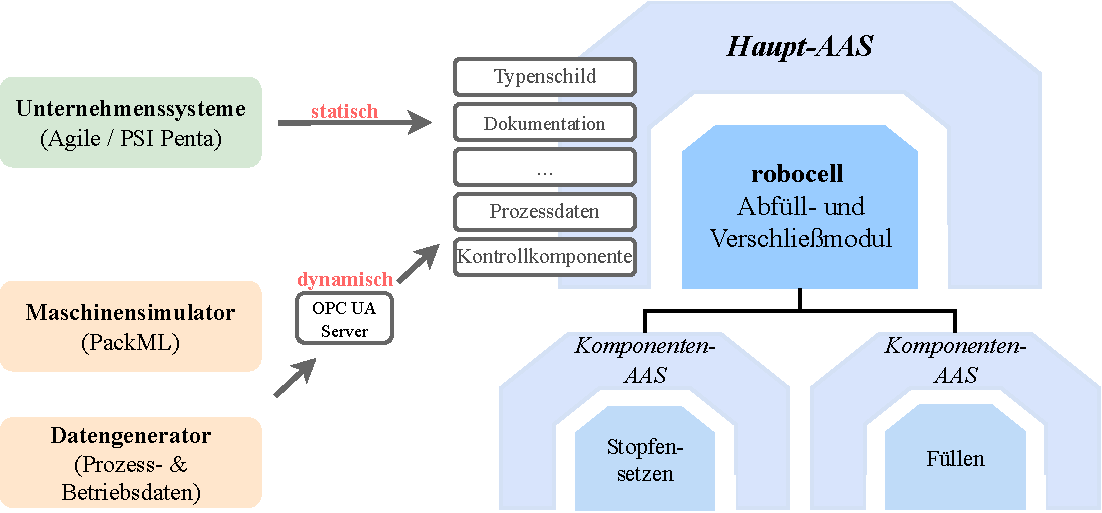
\includegraphics[width=1\textwidth]{Bilder/Konzeptionierung/konzeptionierungNeu.pdf}
%     \caption{\acs{aas}-Konzept der robocell}
%     \label{fig:konzeptionierungAAS}
% \end{figure}

\newpage
\subsection{Modellierung mit der AAS}
In diesem Abschnitt wird beschrieben, wie die zuvor ausgewählten Submodelle in eine \acs{aas} integriert und mit konkreten Daten sowie semantischen Informationen angereichert werden können.
Dabei wird erläutert, wie eine \acs{aas} von Grund auf modelliert, schrittweise mit Inhalten gefüllt und abschließend gespeichert bzw. exportiert werden kann.  
Die Umsetzung erfolgt mithilfe des Package Explorers, der eine intuitive Modellierung aller relevanten Elemente der \acs{aas} ermöglicht und so den strukturierten Aufbau eines digitalen Zwillings unterstützt.
Außerdem wird gezeigt, wie sich die erstellte \acs{aas} mit einer Test Engine auf eine korrekte und vollständige Struktur überprüfen lässt.

\subsubsection{Praktische Umsetzung mit dem Package Explorer}

Die Modellierung beginnt mit dem Erstellen eines neuen \acs{aas}-Pakets im Package Explorer.
Dieses dient als Container für die digitalen Inhalte eines Assets.  
In der geöffneten Umgebung lässt sich eine neue \acs{aas} anlegen, die sowohl allgemeine als auch assetspezifische Daten enthält. 
Abbildung~\ref{fig:NeuesAASPaket} zeigt den initialen Aufbau im Package Explorer, der im weiteren Verlauf sukzessive um Submodelle und deren Inhalte erweitert wird.
Dateien, wie ein Titelbild für die robocell können dabei bereits zu Beginn in die \acs{aas}-Umgebung eingebettet werden und sind ein integraler Bestandteil des digitalen Zwillings.

\begin{figure}[htbp]
    \centering
    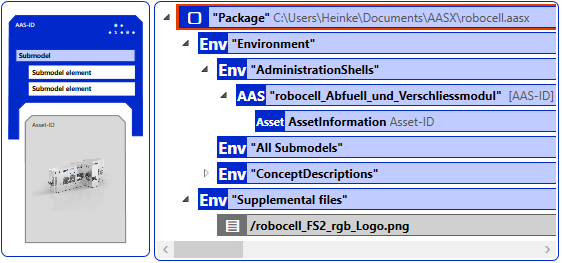
\includegraphics{Bilder/ModellierungAAS/Final/NeuesAASPaket.PNG}
    \caption{AAS-Paket im Package Explorer}
    \label{fig:NeuesAASPaket}
\end{figure}

Zunächst müssen die Metadaten der \acs{aas} sowie des zugehörigen Asset spezifiziert werden.
Neben der Auswahl des Asset-Typs ist insbesondere die eindeutige Identifikation von zentraler Bedeutung.
Das Asset selbst wird über eine globalAssetId referenziert, während die \acs{aas} eine eigene ID und eine idShort erhält.
Diese vereinfachen nicht nur den späteren Austausch der \acs{aas}, sondern ermöglichen auch deren systemweites Auffinden innerhalb eines Industrie-4.0-Ökosystems.
Für erste Modellierungszwecke empfiehlt es sich, auf automatisch generierte Beispiel-IDs zurückzugreifen, die direkt im Package Explorer erzeugt werden können.

\subsubsection*{Strukturierung durch Submodelle}
Im nächsten Schritt müssen die benötigten Submodelle zur \acs{aas} hinzugefügt werden.
Diese lassen sich entweder als Instanz, Typ oder auch Template anlegen, was eine flexible Modellierung je nach Anwendungsfall ermöglicht.
Jedes Submodell erhält dabei wie die \acs{aas} auch eine eindeutige ID, über die diese später identifiziert werden können.
Zusätzlich können optionale Administrationsinformationen angegeben werden, wie beispielsweise die Versionsnummer oder der Name des Autors.

Beim Erstellen eines Submodells ist dieses zunächst leer. 
Die Modellierung erfolgt durch das schrittweise Hinzufügen von Submodellelementen.
Tabelle~\ref{tab:Submodellelemente} gibt einen Überblick über die wichtigsten Submodellelemente, die im Package Explorer zur Verfügung stehen.
Gemäß der Metamodellspezifikation \cite{SpezifikationPart1} wird dabei zwischen DataElements und SubmodelElements unterschieden.
DataElements bilden stets die unterste Ebene im Modell. Sie enthalten konkrete Informationen wie Werte oder Dateien und können keine weiteren Elemente enthalten.
SubmodelElements hingegen sind komplexere Strukturen die wiederum als Container für untergeordnete Elemente dienen.

{\small
\begin{longtblr}[
    label = tab:Submodellelemente,
    entry = Submodellelemente im Package Explorer,
    caption = {Submodellelemente im Package Explorer nach \cite{SpezifikationPart1}},
  ]{
    colspec = {l l X[l]},
    cell{1}{1} = {c=2}{},
    cell{2}{1} = {r=6}{c},
    cell{2}{1} = {bg=babyblue},
    cell{8}{1} = {r=6}{c},
    cell{8}{1} = {bg=babyblue},
    rowhead = 1,
    vline{1,3,4,5} = {-}{},
    vline{2} = {-}{},
    hline{1-2,8,14} = {-}{},
    hline{3-8,9-13} = {2-3}{}, 
    row{1} = {bg=tableHeader},
    }
    \textbf{\makecell[l]{Submodellelement}}& & \textbf{Beschreibung}\\
    \begin{sideways}DataElement\end{sideways}   &Blob & Binärdatei                                                                   \\
    &\makecell[l]{File} & \makecell[l]{Verlinkte oder eingebettete Datei mit \\ eindeutigem MIME-Type}                                                                 \\
    &\makecell[l]{MultiLanguage-\\Property} & Property mit mehrsprachigen Inhalten                              \\
    &Property & Einfaches Merkmal mit festem Datentyp                    \\
    &Range & Wertebereich mit Minimal- und Maximalwert                                                                  \\
    &\makecell[l]{Reference-\\Element} & Verweis auf interne oder externe Elemente                                     \\
    \begin{sideways}SubmodelElement\end{sideways} &Capability & \makecell[l]{Fähigkeit eines Assets, etwas bewirken \\ zu können (ohne konkrete Umsetzung)}                                                            \\
    &Entity & \makecell[l]{Einzelne Komponente (Asset) innerhalb \\ einer übergeordneten AAS  }                                                              \\
    &Operation & \makecell[l]{Funktion mit Ein- und Ausgabeparametern, die \\ von einem System ausgeführt werden kann}                                                               \\
    &\makecell[l]{Relationship-\\Element} & \makecell[l]{Beziehung zwischen zwei Elementen \\(sowohl intern als auch extern möglich)}                                   \\
    &\makecell[l]{Submodel-\\ElementList (\acs{sml})} & \makecell[l]{Geordnete Liste verschiedener Submodellelemente}                                 \\
    &\makecell[l]{SubmodelElement-\\Collection (\acs{smc})} & Sammlung von Submodellelementen                           \\
\end{longtblr}
}

Submodellelemente erhalten im Gegensatz zu Submodellen keine eigene ID, sondern werden über ihre idShort eindeutig referenziert.
Diese muss innerhalb eines Submodells einzigartig sein.
Eine Ausnahme bilden \acsp{sml}, in denen die enthaltenen Elemente nicht über eine idShort, sondern nur über ihre Position (Index) identifiziert werden.

% Ein weiterer wichtiger Punkt sind Referenzen im Package Explorer.
% Vlt bekomme ich auch nochmal Entitäten rein


Alternativ zur manuellen Modellierung können die im Rahmen der Konzeption ausgewählten \acsp{smt} verwendet werden, wie sie in Tabelle~\ref{tab:Submodelle} aufgeführt sind.
Diese stammen beispielsweise aus dem offiziellen Repository der \acs{idta} \cite{idtaTemplates} und lassen sich als AASX-Dateien importieren.
Im Package Explorer erfolgt dies über ein sogenanntes Auxiliary AAS, das als sekundäre Umgebung zur Template-Verwaltung dient.
Die importierten Templates enthalten eine strukturierte Vorlage mit typischen Submodellelementen und reduzieren somit den Modellierungsaufwand erheblich.
Auch unternehmensspezifische Ableitungen lassen sich darauf aufbauend erstellen.
Ein vertiefter Ansatz zur Template-Nutzung findet sich in Kapitel~\ref{chap:ErstellenvonSubmodelTemplates}.

Nach dem Strukturaufbau können konkrete Inhalte wie Werte, Dokumente oder Referenzen eingepflegt werden.
Dies beschränkt sich jedoch auf statische Submodelle wie Technische Daten oder Dokumentation.
Dynamische Inhalte, etwa Betriebsdaten werden nicht direkt im Package Explorer gepflegt, sondern über externe Datenquellen (z.B. Maschinensimulator oder Datengenerator) angebunden.

Abbildung \ref{fig:SubmodellTypenschild} veranschaulicht den strukturellen Aufbau im Package Explorer. 
Gezeigt wird ein Ausschnitt des statischen Submodells Typenschild.

\begin{figure}[htbp]
    \centering
    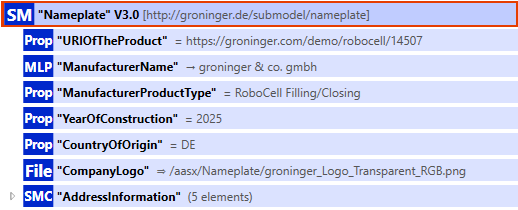
\includegraphics{Bilder/ModellierungAAS/Final/Submodell.PNG}
    \caption{Package Explorer: Ausschnitt Submodell Typenschild}
    \label{fig:SubmodellTypenschild}
\end{figure}

\subsubsection*{Semantische Beschreibung mit Concept Descriptions}

Für die semantische Beschreibung von Submodellen und Submodellelementen innerhalb der AAS ist die Vergabe von semanticId-Referenzen essenziell.
Jede semanticId verweist auf eine zugehörige \acs{cd}, die die Bedeutung des referenzierten Elements eindeutig und maschinenlesbar beschreibt.
Im Package Explorer lassen sich solche Concept Descriptions manuell anlegen und verwalten.
Dabei steht eine vordefinierte Eingabemaske zur Verfügung, die sich an dem in Part 3a: Data Specification - IEC 61360 \cite{SpezifikationPart3a} vordefinierten Datenmodell für semantische Beschreibungen orientiert.
Die Grundstruktur dieser Vorlage ist bei allen Elementen der \acs{aas} gleich.
Allerdings unterscheiden sich je nach Elementtyp die verpflichtenden und empfohlenen Felder.
Das bedeutet, dass für verschiedene Elemente (z.B. Property oder Relationship) jeweils unterschiedliche Felder als zwingend erforderlich gelten, während andere optional oder gar nicht vorgesehen sind.
Die Struktur wird im Folgenden am Beispiel einer Property für die physikalische Größe Frequenz dargestellt.

\begin{tcolorbox}[colframe=black, colback=white, boxrule=0.8pt, arc=4pt, left=8pt, right=8pt, top=8pt, bottom=8pt]
\noindent
\begin{minipage}[t]{0.48\textwidth}
\begin{description}[style=unboxed,leftmargin=3cm,labelsep=0.2cm]
  \item[preferredName:] Frequency \mandatory
  \item[shortName:] freq \recommended
  \item[unit:] Hz \recommended
  \item[unitId:] IEC ... \recommended
  \item[sourceOfDefinition:] - \optional
  \item[symbol:] f \optional
  \item[dataType:]REAL\_MEASURE \mandatory
\end{description}
\end{minipage}%
\hfill
\begin{minipage}[t]{0.48\textwidth}
\begin{description}[style=unboxed,leftmargin=3cm,labelsep=0.2cm]
  \item[definition:] Nominal frequency ... \recommended
  \item[valueFormat:] f \optional
  \item[valueList:] \notused
  \item[value:] 50 \mandatory
  \item[valueId:] VAL001 \optional
  \item[levelType:] \notused
\end{description}
\end{minipage}
\end{tcolorbox}

\begin{tcolorbox}[legendbox]
\mandatory\ Pflichtfeld \quad
\recommended\ Empfohlen \quad
\optional\ Optional \quad
\notused\ Nicht vorgesehen
\end{tcolorbox}

Alternativ können auch externe Standards referenziert werden. 
Der Package Explorer unterstützt diesen Ansatz durch eine erweiterte Funktionalität, mit der sich vorgefertigte ECLASS-Kataloge direkt in das Tool importieren lassen. 
Nach dem Import können die enthaltenen Objekte durchsucht, ausgewählt und den entsprechenden Submodellen oder Submodellelementen zugewiesen werden. 
Die semantische Verknüpfung erfolgt dabei über eine \acs{irdi}, die das jeweilige Konzept eindeutig identifiziert \cite{eclass_irdi}. 

Wird ein solcher Standard referenziert, legt der Package Explorer automatisch eine \acs{cd} an.
Diese folgt, wie bei der manuellen Erstellung, dem in IEC~61360 definierten Datenmodell.  
So sind die semantischen Informationen auch lokal im Modell verfügbar und konsistent strukturiert.
Technisch betrachtet wäre jedoch auch eine rein externe Referenz ausreichend, da die entsprechenden Elemente bereits vollständig in den jeweiligen Katalogen enthalten sind.
Die Nutzung etablierter externer Standards ist grundsätzlich zu bevorzugen, da sie nicht nur den Modellierungsaufwand erheblich reduziert, sondern auch die Interoperabilität zwischen verschiedenen Systemen und Anwendungen deutlich verbessert.

\subsubsection*{Exportmöglichkeiten im Package Explorer}
Nach Abschluss der Modellierung lässt sich die erstellte \acs{aas} in verschiedenen Formaten exportieren.
Das bevorzugte Format in diesem Projekt ist das AASX-Format, das sich als standardisierte Austauschform für die \acs{aas} etabliert hat.
Es enthält alle modellierten Inhalte, einschließlich eingebetteter Dateien wie Bilder oder Dokumente, und eignet sich daher besonders für die Weitergabe einer Typ-1-\acs{aas}.

Alternativ kann die \acs{aas} auch als JSON- oder XML-Datei gespeichert werden.
Diese Formate beeinhalten allerdings ausschließlich die strukturierte Beschreibung der \acs{aas}, eignen sich jedoch besonders für die Nutzung in APIs oder zur Anbindung an bestehende Softwaresysteme.
Zusätzlich unterstützt der Package Explorer auch den gezielten Export einzelner Submodelle oder Concept Descriptions.
Diese lassen sich seperat, etwa als JSON-Datei abspeichern und können so gezielt in anderen AAS-Projekten wiederverwendet werden.

% \subsubsection{Abbildung hierarchischer Strukturen und Beziehungen}
% Zur Abbildung hierarchischer Strukturen, insbesondere im Submodell \acs{bom}, werden sogenannte Entities verwendet. 
% Eine Entitie repräsentiert dabei ein untergeordnetes Asset innerhalb der Gesamtstruktur. 
% Grundsätzlich lassen sich zwei Typen unterscheiden. 
% CoManagedEntities besitzen keine eigene \acs{aas} und werden innerhalb der AAS der übergeordneten Hauptkomponente mitverwaltet. 
% SelfManagedEntities hingegen, wie sie im Rahmen der Konzeption dieser Arbeit vorgesehen sind, verfügen über eine eigene \acs{aas} und können somit unabhängig verwaltet und referenziert werden. 
% Die Identifikation erfolgt über die jeweils zugewiesene globalAssetId.

\subsubsection{Validierung}
Im Anschluss an die Modellierung der \acs{aas} sollte eine Überprüfung der Konformität erfolgen.
Hierzu kann eine von der \acs{idta} bereitgestellte Test Engine \cite{TestEngine} eingesetzt werden. 
Diese lässt sich direkt mit pip, dem Paktemanager von Python, installieren und anschließend über die Kommandozeile nutzen.
Mit dem Befehl \tcbox[inlinebox]{\texttt{aas\_test\_engines check\_files robocell.aasx}} kann beispielsweise die Validierung der zuvor erstellten AASX-Datei der robocell gestartet werden.

Dabei wird zunächst geprüft, ob die AASX-Datei formal korrekt aufgebaut ist, insbesondere hinsichtlich der internen Struktur und ihrer Beziehungen.
Anschließend erfolgt die Kontrolle der enthaltenen \acs{aas} gegen die Metamodell-Spezifikationen der \acs{idta} (Teil 1 \cite{SpezifikationPart1} und 3a \cite{SpezifikationPart3a}).
Zuletzt erfolgt ein Abgleich der Submodelle mit den zugehörigen Templates, sofern diese für das jeweilige Submodell definiert wurden.

Treten bei der Validierung formale oder semantische Fehler auf, beispielsweise durch fehlende Referenzen oder ungültige IDs, gibt die Test Engine eine detaillierte Fehlermeldung in der Konsole aus. 
Diese Hinweise geben Aufschluss darüber, an welcher Stelle die Struktur bzw. der Inhalt der AASX-Datei fehlerhaft ist, und ermöglichen so eine gezielte Korrektur der betroffenen Elemente. 
Werden im gesamten Prüfprozess hingegen keine Fehler oder Abweichungen festgestellt, bestätigt die Test Engine die erfolgreiche Validierung.

\newpage
\subsection{Technische Integration}
Im Anschluss an die Konzeption und Modellierung des digitalen Zwillings liegt der Fokus dieses Kapitels auf der technischen Integration der zuvor erstellten \acs{aas} in eine Industrie-4.0-kompatible Umgebung.
Dabei wird unter anderem gezeigt, wie die statisch modellierte Typ-1-\acs{aas} mithilfe des AASX Server Blazor beziehungsweise vorzugsweise der Eclipse BaSyx-Plattform in eine Typ-2-\acs{aas} überführt und systemseitig bereitgestellt werden kann.
Ergänzend dazu wird beschrieben, wie die \acs{aas} um dynamische Inhalte erweitert werden kann.
Dies umfasst die Integration von Echtzeitdaten über OPC UA sowie die Einbindung und Visualisierung externer Zeitreihendaten mithilfe von InfluxDB und Telegraf.

\subsubsection{Bereitstellung der \acs{aas}}
\label{sec:bereitstellungAAS}
Für die Bereitstellung als Typ-2-\acs{aas} stehen verschiedene Open-Source-Lösungen zur Verfügung. 
Eine besonders einsteigerfreundliche Option stellt der AASX Server Blazor \cite{AASXServer} dar.
Er bildet das serverseitige Gegenstück zum Package Explorer und verfügt ebenfalls über eine grafische Benutzeroberfläche zur Visualisierung von \acs{aas}-Paketen.
Über eine HTTP-Schnittstelle können die beiden Anwendungen miteinander verbunden werden.
Dadurch lassen sich AASX-Dateien ohne zusätzlichen Konfigurationsaufwand direkt aus dem Package Explorer heraus auf den Server übertragen und bereitstellen.
Ebenso können auf dem Server gespeicherte \acs{aas} über den Explorer eingesehen und bearbeitet werden.
Die enge Verzahnung beider Komponenten ermöglicht somit eine unkomplizierte Bereitstellung und Verwaltung von \acs{aas}-Paketen und eignet sich besonders für erste Testszenarien oder prototypische Anwendungen.

Für komplexere Anwendungsszenarien, insbesondere solche mit Anforderungen an Echtzeitfähigkeit sowie an flexible und erweiterbare Submodelle, stößt der AASX Server Blazor jedoch an seine funktionalen und architektonischen Grenzen. 
So fehlen beispielsweise Schnittstellen zur Anbindung dynamischer Datenquellen sowie Möglichkeiten zur Skalierung und zur verteilten Systemintegration.
Aus diesem Grund wird im weiteren Verlauf dieses Projekts die Eclipse BaSyx-Plattform eingesetzt.
Durch ihre modulare Architektur und die klare Trennung verschiedener Komponenten wie den Registries oder den Repositories bietet sie eine deutlich flexiblere Grundlage für die Umsetzung anspruchsvoller Industrie 4.0-Szenarien.

Die einfachste Möglichkeit, BaSyx zu installieren, besteht in der Nutzung von Docker.
Alle benötigten Komponenten stehen als vorgefertigte Images öffentlich über den Docker Hub zur Verfügung. 
Alternativ kann der Quellcode von GitHub bezogen werden, um einzelne Komponenten individuell anzupassen oder zu erweitern.
Die verschiedenen Services, darunter die \acs{aas} Environment, Registries für \acs{aas} und Submodelle, der Discovery Service, sowie die MongoDB als persistenter Speicher, können zentral in einer docker-compose.yml-Datei verwaltet werden.
Die Konfiguration erfolgt in der Regel über Umgebungsvariablen oder seperate Konfigurationsdateien, die in der docker-compose.yml referenziert werden.
Mit dem Befehl docker compose up lassen sich anschließend alle Komponenten gemeinsam starten.

Nach erfolgreichem Start der BaSyx-Umgebung stehen verschiedene Möglichkeiten zur Verfügung, um eine \acs{aas} bereitzustellen und in das System zu integrieren. 
Welche Methode dabei zum Einsatz kommt, hängt stark von den jeweiligen Anforderungen und Rahmenbedingungen des Anwendungsszenarios ab.
Nachfolgend werden drei ausgewählte Ansätze zur Bereitstellung näher betrachtet.

\noindent\textbf{A. Volume}\\
Eine besonders einfache Variante besteht darin, eine AASX-Datei in ein gemountetes Volume der AAS Environment abzulegen.
Ein Volume ist ein persistentes Speicherverzeichnis auf dem Host-System, das mit einem Verzeichnis innerhalb eines Docker-Containers verknüpft ist.
Es ermöglicht die dauerhafte Speicherung von Daten, unabhängig vom Lebenszyklus des Containers.
In der von Eclipse BaSyx bereitgestellten Docker-Umgebung ist ein entsprechendes Volume in der Regel bereits vorkonfiguriert.

Beim Neustart der AAS Environment wird die AASX-Datei automatisch erkannt, registriert und in das BaSyx-System eingebunden.
Die dabei erzeugten Daten, darunter Informationen zu \acs{aas}, Submodellen, Concept Descriptions sowie Registrierungsdaten, werden in verschiedenen Tabellen der angebunden MongoDB gespeichert.
Dies gewährleistet, dass alle relevanten Daten persistent erhalten bleiben, selbst dann, wenn die ursprüngliche AASX-Datei später wieder aus dem Volume entfernt wird.

\noindent\textbf{B. AAS Web UI}\\
Alternativ kann die Bereitstellung auch direkt über die AAS Web UI erfolgen.
Über die Benutzeroberfläche kann eine AASX-Datei manuell importiert werden, wodurch sie direkt im laufenden System registriert und eingebunden wird.
Diese Methode eignet sich besonders gut für Tests oder kleinere Anpassungen, da eine \acs{aas} auf diese Weise schnell und ohne direkten Zugriff auf das zugrunde liegende Dateisystem eingebunden werden kann.

\noindent\textbf{C. REST-API}\\
Die flexibelste, jedoch auch technisch anspruchsvollste Methode zur Bereitstellung einer AAS ist die manuelle Registrierung über die REST-API. 
Dabei kann nicht einfach eine AASX-Datei hochgeladen werden. 
Stattdessen müssen die AAS, ihre Submodelle sowie deren Beziehungen explizit über die bereitgestellten Schnittstellen des BaSyx-Systems erstellt werden. 
Dies erfolgt durch das Senden strukturierter JSON-Daten im Body der jeweiligen HTTP-Anfragen.
Ein typischer Ablauf dieser Registrierung ist in Tabelle \ref{tab:BereitstellungInBaSyx} dargestellt. 
Sie zeigt die notwendigen Schritte sowie die zugehörigen REST-Endpunkte.
Diese sind dabei verschiedenen Services innerhalb der AAS Environment zugeordnet.

{\small
\begin{longtblr}[
  label = tab:BereitstellungInBaSyx,
  caption = {Bereitstellung einer AAS über die REST-API},
  entry = Bereitstellung einer AAS über die REST-API
]{
  colspec = {l l X},
  rowhead = 1,
  vlines,
  hlines,
  row{1} = {bg=tableHeader}
}
\textbf{Schritt} & \textbf{Service} & \textbf{Endpunkte} \\
1. AAS erstellen & AAS Repository & \texttt{/shells}\\
2. Submodell(e) erstellen & Submodel Repository & \texttt{/submodels}\\
\makecell[l]{3. Submodell(e) mit \\ \acs{aas} verknüpfen} & AAS Repository & \texttt{\makecell[l]{/shells/{\{aasIdentifier\}} \\ /submodel-refs}}\\
4. \acs{cd} anlegen & \acs{cd} Repository & \texttt{/concept-descriptions}\\
\end{longtblr}
}

Neben der Bereitstellung in der AAS Environment kann eine \acs{aas} optional auch im Discovery Service registriert werden.
Über einen sogenannten assetLink kann diese dabei logisch mit ihrem zugehörigen Asset verknüpft werden.
Die Registrierung erfolgt analog zur AAS Environment über einen REST-Endpunkt.
Besonders bei der Darstellung von hierarchischen Strukturen, etwa einer \acs{bom} mit mehreren verschachtelten Assets, hilft der Discovery Service bei der eindeutigen Zuordnung der jeweiligen \acs{aas} zu ihrem physischen Gegenstück.

\subsubsection{Integration von Echtzeitdaten über OPC UA}
Nach der Erstellung der statischen \acs{aas} der robocell und der Integration in das BaSyx-System gilt es nun, diese um dynamische Informationen zu erweitern.
Diese sind essenziell, um den aktuellen Maschinenzustand präzise und in Echtzeit abzubilden.
Die Datenbasis bilden die beiden zuvor vorgestellten Anwendungen, die Maschinen- bzw. Sensordaten über einen \acs{opcua} Server bereitstellen.

Die Integration von Echtzeidaten in die \acs{aas} wird im Folgenden am Beispiel des Submodells Prozessdaten erläutert.
Innerhalb dieses Submodells existieren verschiedene Properties, die jeweils bestimmte Werte, wie beispielsweise den Druck oder die Anzahl abefüllter Einheiten, repräsentieren (siehe Abbildung \ref{fig:SubmodellProzessdaten}). %(siehe Abbildung \ref{fig:UMLSubmodellProcessData}). 
Diese Properties sollen im weiteren Verlauf dynamisch mit den simulierten Werten, die über \acs{opcua} bereitgestellt werden, aktualisiert werden.

\begin{figure}[htbp]
    \centering
    % 0.88
    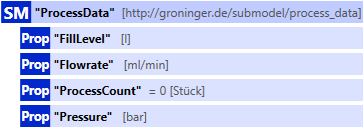
\includegraphics{Bilder/OPCUA/ProcessDataPackageExplorer.PNG}
    \caption{Submodell Prozessdaten}
    \label{fig:SubmodellProzessdaten}
\end{figure}

Das Eclipse BaSyx-Projekt stellt hierfür eine weitere Komponente bereit, die sogenannte Databridge \cite{BaSyxDatabridge}.
Diese steht, wie alle anderen Komponenten auch, als Docker Container zur Verfügung und ermöglicht die Anbindung verschiedenster Datenquellen an eine \acs{aas}.
Sie unterstützt eine Vielzahl von Protokollen, darunter insbesondere auch \acs{opcua} oder MQTT.
Dabei dient sie als Vermittler zwischen einem Datenendpunkt und einem Submodell innerhalb der \acs{aas}.

Die Konfiguration der Databridge erfolgt über mehrere JSON-Dateien.
In einer zentralen Konfigurationsdatei werden sowohl die Datenquelle als auch die Datensenke definiert.
Außerdem können Transformatoren angegeben werden, die beispielsweise Einheitenumrechnungen oder Typkonvertierungen übernehmen.

Als Datenquelle muss der \acs{opcua} Server des Datengenerators angegeben werden, dessen Konfiguration typischerweise in einer separaten JSON-Datei erfolgt.
Darin sind sowohl die Verbindungsparameter des Servers (z.B. URL und Port) als auch die zu überwachenden Knoten anzugeben.
Wie in Abbildung \ref{fig:OPCUADatenStruktur} zu erkennen, stellt der \acs{opcua} Server die Werte hierfür in einer hierarchischen Struktur bereit, wobei jeder Knoten über einen Namespaceindex (ns) und eine NodeId (i) eindeutig adressierbar ist.

\begin{figure}[htbp]
    \centering
    % 0.88
    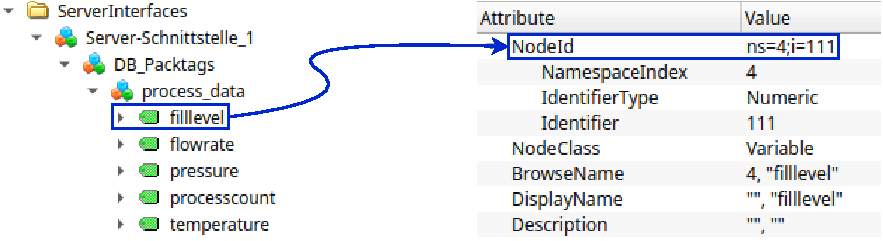
\includegraphics[width=1\textwidth]{Bilder/OPCUA/OPCUADaten.pdf}
    \caption{OPC UA Datenknoten}
    \label{fig:OPCUADatenStruktur}
\end{figure}

Außerdem muss der zu verwendende \acs{opcua} Client festgelegt werden.
In diesem Projekt wird Eclipse Milo eingesetzt, der auf einem Subscription-Modell basiert.
Im Gegensatz zu einem Polling-Ansatz werden hier gezielt bestimmte Knoten (Nodes) abonniert, sodass neue Werte automatisch bei Änderung übermittelt werden.

Ein Beispiel für eine entsprechende JSON-Konfiguration der Datenquelle ist in Listing~\ref{lst:jsonDatenquelle} für den Druckwert dargestellt.
Weitere optionale Parameter, wie etwa Sicherheitseinstellungen oder das Übertragungsintervall können zusätzlich angegeben werden, wurden hier jedoch zur besseren Übersicht weggelassen.

\begin{lstlisting}[language=json, caption={Beispielhafte JSON-Konfiguration einer Datenquelle}, label={lst:jsonDatenquelle}]
{
    "uniqueId"       : "pressure",
    "nodeInformation": "ns=4;i=113",
    "serverUrl"      : "opcua-server",
    "serverPort"     : 4840,
    "pathToService"  : "milo"
}
\end{lstlisting}

Zur Anpassung der eingehenden Daten an die Struktur der Ziel-Property lassen sich verschiedene Transformatoren einsetzen.
Die Databridge unterstützt hierfür unter anderem JSONata-Ausdrücke oder JsonJacksonTransformers.
Mithilfe dieser Mechanismen können die vom \acs{opcua}-Server empfangenen Rohdaten zunächst in ein JSON-Objekt überführt und anschließend gezielt extrahiert und weiterverarbeitet werden.

Im Anschluss erfolgt die Konfiguration der Datensenke, also der Zielkomponente innerhalb der \acs{aas}.
Auch diese erfolgt über eine separate JSON-Datei, in der der Endpunkt des Submodells, der idShortPath der gewünschten Property sowie die verwendete API-Version definiert werden.
Listing~\ref{lst:jsonDatensenke} zeigt ein Beispiel einer entsprechenden Konfiguration.
Der Platzhalter \{smId\} steht dabei für die Base64-kodierte ID des Submodells Prozessdaten, wie sie in der REST-API der \acs{aas} verwendet wird.
\begin{lstlisting}[language=json, caption={Beispielhafte JSON-Konfiguration einer Datensenke}, label={lst:jsonDatensenke}]
{
    "uniqueId"        : "Submodel/ProcessData/Pressure",
    "submodelEndpoint": "http://aas-env:8081/submodels/{smId}",
    "idShortPath"     : "Pressure",
    "api"             : "DotAAS-V3"
}
\end{lstlisting}

Nach erfolgreicher Konfiguration übernimmt die Databridge die automatisierte Übertragung der \acs{opcua}-Werte in die entsprechenden Properties des Submodells.
Dieses Prinzip lässt sich nicht nur auf Prozesswerte anwenden, sondern auch zur Abbildung des Maschinenzustands oder anderer dynamischer Betriebsdaten nutzen.
Somit bildet die Databridge eine flexible und protokolloffene Lösung zur Echtzeitanbindung externer Datenquellen an eine \acs{aas}.


\subsubsection{Verarbeitung von Zeitreihendaten}

Grundsätzlich lassen sich Zeitreihendaten auf unterschiedlichste Weise in eine \acs{aas} einbinden.
Das \acs{smt} Time Series Data \cite{SpezifikationTimeSeriesData} bietet hierfür mehrere standardisierte Lösungsansätze.
Eine Möglichkeit besteht darin, diese direkt über ein InternalSegment in der \acs{aas} zu speichern.
Diese Variante eignet sich jedoch nur für kleinere Datenmengen.
Alternativ können die Daten in Form einer Datei abgespeichert werden.
Diese können dann entweder direkt in die \acs{aas} eingebunden oder extern über ein ExternalSegment referenziert werden.
Für größere Datenmengen bietet sich die exterene Speicherung an einem seperaten Ort, wie etwa einer Datenbank, an.
Diese kann über ein LinkedSegment mit der \acs{aas} verknüpft werden.

Im Folgenden wird die zuletzt genannte Option näher betrachtet.
Hierzu werden die simulierten Werte für Druck und Temperatur des Datengenerators extern in einer InfluxDB gespeichert.
Die über \acs{opcua} bereitgestellten Daten werden dabei mithilfe von Telegraf, einem leichtgewichtigen Agenten zur Datenerfassung und -weiterleitung \cite{Influx}, kontinuierlich in eine speziell für diesen Anwendungsfall angelegte Tabelle geschrieben.
InfluxDB sowie Telegraf stehen dabei beide als Docker-Container zur Verfügung und lassen sich so nahtlos in das bestehende BaSyx-System integrieren.

Um die in der Datenbank gespeicherten Daten in die \acs{aas} einzubinden, kann das bereits genannte \acs{smt} Time Series Data verwendet werden.
Zunächst müssen die Metadaten eingetragen werden (siehe Abbildung \ref{fig:MetadataTimeSeries}).
Dazu gehören ein eindeutiger Name, eine Beschreibung sowie die Definition der Datenpunkte (Records), die hiermit aufgezeichnet werden sollen.

\begin{figure}[htbp]
    \centering
    % 0.88
    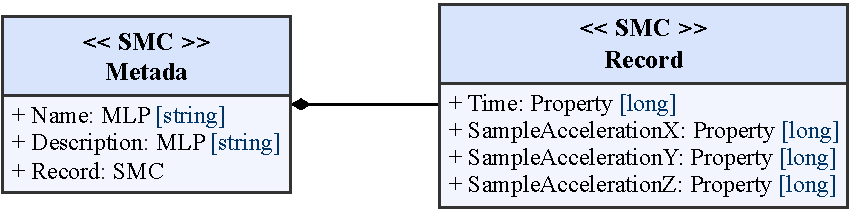
\includegraphics[width=1\textwidth]{Bilder/TimeSeries/Metadaten.pdf}
    \caption{Metadaten im Submodell Time Series Data}
    \label{fig:MetadataTimeSeries}
\end{figure}

Anschließend folgt die Konfiguration des LinkedSegments (siehe Abbildung \ref{fig:LinkedSegmentTimeSeries}). 
Dieses stellt die eigentliche Verbindung zu den extern gespeicherten Zeitreihendaten her.
Hierfür sind sowohl der Datenendpunkt als als auch die Query, mit der die gewünschten Werte ausgelesen werden sollen, zu spezifizieren.
Im vorliegenden Fall handelt es sich dabei um die Adresse des InfluxDB-Containers sowie die Abfrage, mit der die Werte für Druck und Temperatur aus der zugehörigen Tabelle extrahiert werden können.
Dabei ist zu beachten, dass der entsprechende Port der InfluxDB nach außen freigegeben ist, da andernfalls kein Zugriff durch externe Anwendungen möglich ist.
Ergänzend können weitere Metadaten angegeben werden, beispielsweise die Abtastrate (samplingRate), der durch das Segment abgedeckte Zeitraum oder ein recordCount, der die erwartete Anzahl an Einträgen innerhalb dieses Zeitfensters beschreibt.

\begin{figure}[htbp]
    \centering
    % 0.86
    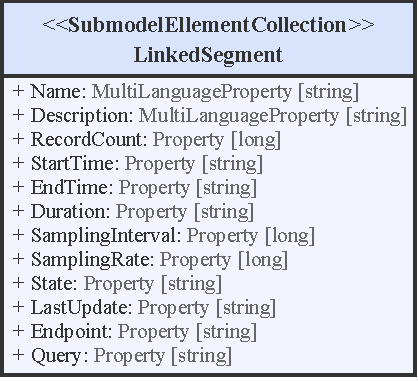
\includegraphics{Bilder/TimeSeries/LinkedSegment.pdf}
    \caption{LinkedSegment im Submodell Time Series Data}
    \label{fig:LinkedSegmentTimeSeries}
\end{figure}

Zur Visualisierung der Zeitreihendaten bietet das BaSyx-System eine praktische Lösung.
Über ein entsprechendes Plugin können die im Submodell Time Series Data enthaltenen Informationen direkt in der Benutzeroberfläche der AAS Web UI dargestellt werden.
Die über das LinkedSegment referenzierten Zeitreihendaten lassen sich dort in verschiedenen Diagrammen visualisieren, beispielsweise als Linien- oder Balkendiagramm.
Dadurch wird eine benutzerfreundliche Darstellung der Daten ermöglicht, ohne dass diese physisch in der \acs{aas} gespeichert werden müssen.

\newpage
\subsection{Anwendungsfall Digitaler Produktpass}
Im Kontext steigender Anforderungen an Nachhaltigkeit und Transparenz entlang des gesamten Produktlebenszyklus eines Assets gewinnt der \acs{dpp} zunehmend an Bedeutung. 
Der Fokus dieses Anwendungsfalls liegt auf zwei zentralen Aspekten: der Abbildung des \acs{pcf} sowie der technischen Umsetzung von Zugriffsrechten auf die im \acs{dpp} enthaltenen Daten.

Der \acs{pcf} beschreibt die Summe aller Treibhausgasemissionen, ausgedrückt in CO\textsubscript{2}-Äquivalenten, die entlang des Lebenszyklus eines Produkts entstehen \cite{PCF}. 
Seine Bedeutung zeigt sich auch in der EU-Batterieverordnung \cite{EUVerordnung}, die die Einführung eines digitalen Batteriepasses vorschreibt, der die erste konkrete Umsetzung eines \acs{dpp} darstellt und daher als Ausgangspunkt für weitere Branchen wie den Maschinen- und Anlagenbau dient.
Darin wird unter anderem die verpflichtende Angabe des \acs{pcf}, insbesondere für die Phasen Material, Produktion und die Gesamtbetrachtung (Cradle to Gate) gefordert, welche im Rahmen dieses Anwendungsfalls exemplarisch umgesetzt werden. 
Für weiterführende Lebenszyklusphasen wie die Nutzung ist die Angabe derzeit noch nicht vorgeschrieben.

Die technische Umsetzung orientiert sich an dem vom ZVEI vorgestellten Konzept des \acs{dpp40}, das gemeinsam mit der \acs{idta} im Rahmen eines \acs{pcf}-Showcases demonstriert wird \cite{PCFShowcas}. 
Aufbauend auf diesem Konzept wird gezeigt, wie ein \acs{dpp} mithilfe der \acs{aas} modelliert und prototypisch realisiert werden kann.

Konkret wird der digitale Zwilling des Abfüll- und Verschließmoduls der robocell um ein Submodell zur Abbildung des \acs{pcf} erweitert. 
Der Fokus liegt auf der exemplarischen Aggregation von CO\textsubscript{2}-Daten aus Zulieferkomponenten, um den \acs{pcf} des Moduls zu berechnen. 
Ergänzend wird demonstriert, wie sich Zugriffsrechte auf die im \acs{dpp} enthaltenen Informationen mithilfe der Eclipse BaSyx-Plattform umsetzen lassen.

\subsubsection{Umsetzung mit dem Teilmodell Carbon Footprint}
Zur exemplarischen Abbildung und dynamischen Berechnung des \acs{pcf} der Gesamtmaschine wird das von der \acs{idta} spezifizierte \acs{smt} \acs{cf} \cite{SpezifikaitonPCF} eingesetzt.  
Dieses Template definiert eine standardisierte Struktur zur Erfassung von CO\textsubscript{2}-Äquivalenten entlang des Produktlebenszyklus.  
Es unterscheidet zwischen dem \acs{pcf} und dem Transport Carbon Footprint (TCF), wobei im Rahmen dieses Anwendungsfalls ausschließlich der \acs{pcf} betrachtet wird.

Das \acs{smt} gibt die Struktur des \acs{pcf} in Form einer \acs{smc} vor.  
Diese Sammlung enthält standardisierte Elemente wie den CO\textsubscript{2}-Wert, die zugehörige Lebenszyklusphase, die verwendete Berechnungsmethode sowie den Gültigkeitszeitraum.
Wie bereits zuvor beschrieben, liegt der Fokus auf den Lebenszyklusphasen Material, Produktion und Cradle to Gate.  
Für jede dieser Phasen empfiehlt es sich, eine eigene \acs{smc} gemäß der Submodellspezifikation zu erstellen.  
Diese Sammlungen dienen als Basis für die spätere Aggregation der \acs{pcf}-Werte der Gesamtmaschine und werden im weiteren Verlauf dynamisch mit Werten befüllt.

Für die exemplarische Berechnung des \acs{pcf} wurde eine Auswahl an Steuerungskomponenten festgelegt, die in der robocell verbaut sind.  
Diese Auswahl beschränkt sich auf Siemens-Komponenten, darunter beispielsweise eine CPU sowie Ein- und Ausgangsmodule.  
Die Komponenten wurden als Typ-1-\acs{aas} zur Verfügung gestellt, wobei jede \acs{aas} ein eigenes Submodell gemäß des \acs{smt} \acs{cf} enthält.

Um diese in die \acs{pcf}-Berechnung einzubeziehen, können sie direkt im \acs{cf}-Submodell der robocell referenziert werden. 
In diesem Anwendungsfall erfolgt dies über eine \acs{sml}, in der die Komponenten als Entities unter Angabe ihrer jeweiligen globalAssetId eingebunden sind. 
Alternativ wäre auch eine Referenzierung direkt über das \acs{bom}-Submodell möglich.

Für die dynamische Berechnung müssen sowohl die \acs{aas} der robocell als auch die zugehörigen Komponenten-\acs{aas} in einer Laufzeitumgebung verfügbar sein. 
Die Bereitstellung erfolgt über die Eclipse BaSyx-Plattform.
Zur Benutzerinteraktion wird das bestehendes Vue.js-Plugin für den Carbon Fooprint der AAS Web UI genutzt.
Dieses wird im Rahmen dieses Anwendungsfalls um eine Schaltfläche zur Initialisierung der Aggregation erweitert wird.

Die Aggregationslogik ist als eigenständiger, Node.js-basierter Microservice mit einer Web-API implementiert. 
Diese wertet die Komponenten-\acs{aas} aus, berechnet die aggregierten Werte für die zuvor definierten Lebenszyklusphasen und schreibt diese in das \acs{cf}-Submodell der Haupt-AAS der robocell zurück. 
Die Auslösung des Microservice erfolgt über die Schaltfläche im erweiterten Plugin.

Alternativ wäre auch eine clientseitige Berechnung direkt im \acs{cf}-Plugin denkbar. 
In der vorliegenden Umsetzung liegt die gesamte Aggregationslogik jedoch zentral und serverseitig im Microservice. 
Der Ablauf ist in Abbildung \ref{fig:SequenzdiagrammPCF} als Sequenzdiagramm dargestellt.

\newpage
\begin{figure}[htbp]
    \centering
        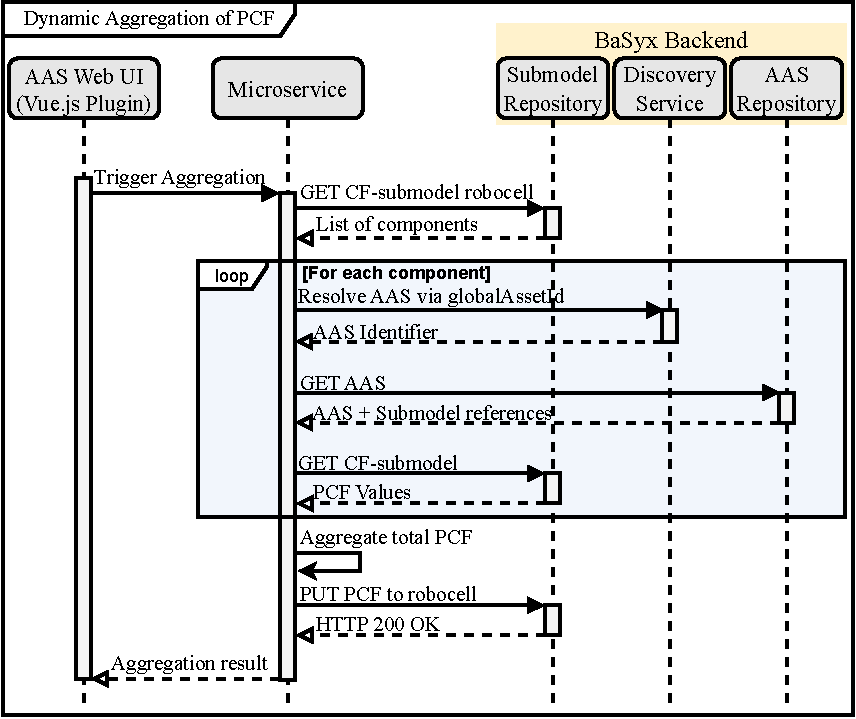
\includegraphics[width=1\textwidth]{Bilder/DPP/Sequenzdiagramm_Neu.pdf}
    
    \caption{Sequenzdiagramm zur Aggregation des PCF}
    \label{fig:SequenzdiagrammPCF}
\end{figure}

Der Microservice nutzt die REST-Schnittstelle des Submodel Repositories der AAS Environment, um zunächst alle in der \acs{aas} der robocell hinterlegten Komponenten auszulesen. 
Mithilfe des Discovery Service werden auf Basis ihrer globalAssetIds die zugehörigen Komponenten-\acs{aas} identifiziert und anschließend vom AAS Repository abgerufen.
Für jede dieser Komponenten wird geprüft, ob ein \acs{cf}-Submodell vorhanden ist. 
Falls dies zutrifft, wird das Submodell ausgelesen und die enthaltenen Werte extrahiert.

Aus den ermittelten Einzelwerten berechnet der Microservice schließlich die aggregierten CO\textsubscript{2}-Äquivalente für die Phasen Produktion, Material sowie Cradle to Gate. 
Die berechneten Werte werden abschließend in das \acs{cf}-Submodell der Haupt-\acs{aas} der robocell geschrieben und stehen dort strukturiert zur Verfügung.

\subsubsection{Zugriffsrechte und Datensicherheit}
Die kontrollierte Bereitstellung der im \acs{dpp} enthaltenen Daten spielt eine zentrale Rolle, insbesondere im Hinblick auf Datenschutz, regulatorische Anforderungen sowie den Schutz gesitigen Eigentums. 
Wie in Kapitel~\ref{sec: Sicherheit} beschrieben, sieht die Security-Spezifikation der \acs{idta} die Nutzung eines \acs{abac}-Ansatzes vor, um eine feingranulare Zugriffskontrolle auf Submodelle und deren Elemente zu ermöglichen.
Da sich die \acs{abac}-Funktionalität in gängigen Implementierungen wie dem AASX Server Blazor oder Eclipse BaSyx derzeit noch in der Entwicklung befindet, wird die Umsetzung der Zugriffsrechte im Rahmen dieses Anwendungsfalls exemplarisch anhand eines \acs{rbac}-Ansatzes demonstriert, wie er in Eclipse BaSyx unterstützt wird.


Groninger-Mitarbeiter
Kunde
Service-Techniker

% Für den Anwendungsfall des \acs{dpp} werden exemplarisch zwei Rollen definiert:
%     \item \textbf{Groninger-Mitarbeiter}: Diese Rolle erhält Vollzugriff auf den \acs{dpp}. Sie kann Werte einsehen, aktualisieren und auch wieder löschen.
%     \item \textbf{Externer Kunde}: Diese Rolle erhält ausschließlich Leserechte auf ausgewählte Submodelle.
% \end{itemize}




\newpage
\subsection{Anwendungsfall automatisierte Generierung von AAS}
Ziel dieses Anwendungsfalls ist es, den Prozess der automatisierten Generierung und Bereitstellung einer \acs{aas} exemplarisch darzustellen. 
Hierzu wird im ersten Schritt ein unternehmensspezifisches \acs{smt} erstellt, das anschließend in ein Typ-Submodell überführt wird.
Dieses bildet die Grundlage für die automatisierte Generierung eines Instanz-Submodells, das mit konkreten Daten befüllt, in eine \acs{aas} eingebettet und schließlich in das BaSyx-System integriert wird.

\subsubsection{Arbeiten mit Submodel Templates}
\label{chap:ErstellenvonSubmodelTemplates}
Für die automatisierte Generierung einer \acs{aas} ist eine konsistente Submodellstruktur erforderlich, die sich aus wiederverwendbaren Vorlagen ableiten lässt.
Im vorliegenden Anwendungsfall dient das standardisierte \acs{smt} Technische Daten \cite{SpezifikaitonTechnischeDaten} als Ausgangspunkt. 
Dieses definiert eine generische Struktur zur Beschreibung technischer Merkmale, gegliedert in Kategorien (\acsp{smc}) wie Generelle Informationen, Technische Informationen oder Produktklassifikation. 
Es bildet somit den semantischen Rahmen, enthält jedoch zunächst keine konkreten Ausprägungen.

Auf Unternehmensebene kann das generische Template an spezifische Anforderungen angepasst werden, beispielsweise für einen bestimmten Maschinentyp wie die robocell.
Branchenspezifische Varianten sind grundsätzlich ebenfalls denkbar, werden in diesem Anwendungsfall jedoch nicht weiter betrachtet.

Die Anpassung kann mithilfe des Package Explorers erfolgen.
Über diesen lässt sich das standardisierte \acs{smt} importieren und anschließend gezielt erweitern.
So können etwa produktspezifische Anforderungen, wie Umgebungsbedingungen oder der Verarbeitungsbereich, mithilfe geeigneter Submodellelemente ergänzt werden.
Das resultierende unternehmensspezifische Template erhält eine eigene semanticId, bleibt jedoch zusätzlich mit der ursprünglichen semanticId des generischen Templates verknüpft, um die Rückverfolgbarkeit zur standardisierten Vorlage sicherzustellen.

Anschließend kann aus dem angepassten Template ein Typ-Submodell abgeleitet werden, das nicht nur die Struktur, sondern bereits allgemeingültige Merkmale einer Produktgruppe enthält, beispielsweise den Einsatzort oder die maximal zulässige Umgebungstemperatur.
Dieses Typ-Submodell dient als Vorlage für die spätere Erstellung konkreter AAS-Instanzen, die anschließend mit produktspezifischen Werten wie einer Seriennummer vervollständigt werden.
Die Verbindung zur ursprünglichen sowie zur unternehmensspezifischen Template-Struktur wird dabei über entsprechende semanticId-Verknüpfungen beibehalten.


\subsubsection{Automatisiertes Befüllen mit strukturierten Daten}
Nach der Erstellung eines Typ-Submodells stellt sich die Frage, wie dieses effizient mit konkreten Produktinformationen befüllt und anschließend in eine vollständige \acs{aas}-Instanz überführt werden kann.

In der industriellen Praxis liegen die benötigten Daten meist bereits strukturiert in bestehenden IT-Systemen wie \acs{plm}- oder \acs{erp}-Lösungen vor.
Da eine direkte Systemintegration im Rahmen dieser Arbeit nicht realisierbar ist, wird der Prozess exemplarisch anhand vordefinierter Beispieldaten demonstriert.
Diese Daten enthalten typische technische Merkmale, wie sie auch in realen Unternehmenssystemen vorzufinden sind, und bilden die Grundlage für die automatisierte Erstellung eines Instanz-Submodells.

Die technische Umsetzung erfolgt über ein Skript, das diese Daten automatisiert in die vorgegebene Submodellstruktur überträgt und anschließend in eine neu erzeugte \acs{aas}-Instanz einbettet.
In diesem Projekt wird dazu die serverseitige JavaScript-Laufzeitumgebung Node.js \cite{nodejs} verwendet, da sie eine einfache Verarbeitung von JSON-Daten sowie eine unkomplizierte Kommunikation mit REST-Schnittstellen ermöglicht. 

Als Basis werden drei zentrale JSON-Komponenten benötigt:

\begin{enumerate}[noitemsep, leftmargin=*, label=\textbf{\arabic*.}]
    \item \textbf{Datenquelle:} Technische Produktinformationen
    \item \textbf{Submodell-Vorlage:} Struktur und Semantik des Submodells
    \item \textbf{AAS-Vorlage:} Aufbau und Struktur der \acs{aas}-Instanz
\end{enumerate}

Die Datenquelle ist hierarchisch aufgebaut und enthält verschachtelte Schlüssel-Wert-Paare. 
Jeder Schlüssel entspricht einem idShort-Wert eines Elements innerhalb der Submodell-Vorlage. 
Diese wiederum ist so konzipiert, dass Platzhalter an den relevanten Stellen eingefügt sind, die bei der Skriptausführung mit den zugehörigen Werten aus der Datenquelle ersetzt werden.

Nach der Befüllung des Instanz-Submodells mit konkreten Werten muss dieses in eine neu erzeugte \acs{aas}-Instanz eingebunden werden.
Die zugrunde liegende \acs{aas}-Vorlage definiert die grundlegende Struktur in einer separaten Datei, enthält jedoch noch keine spezifischen Identifikatoren, wie beispielsweise die eindeutige ID der \acs{aas} oder des zugehörigen Assets.
Um diese hinzuzufügen, können während der Skriptausführung zufällig generierte UUIDv4-Werte an den entsprechenden Stellen in die Vorlage eingefügt werden.

Im letzten Schritt erfolgt die Bereitstellung der AAS-Instanz innerhalb des Eclipse BaSyx-Systems. 
Hierzu kann die \acs{aas} sowie das zugehörige Submodell, analog zur Möglichkeit~C REST-API aus Kapitel~\ref{sec:bereitstellungAAS}, eingebunden und registriert werden.

\subsection{Titel Anwendungsfall KI}

\subsubsection{KI-Modell zur Anomalieerkennung}
Zur Erkennung von Abweichungen im Betriebsverhalten der robocell, wird ein KI-basiertes Verfahren auf Basis eines Autoencoders implementiert.
Dieses dient der frühzeitigen Identifikation von Anomalien in Zeitreihendaten.


FÜr die Umsetzung gibt es verschiedene Möglichkeiten. In dieser Arbeit wird pytorch 




Die Umsetzung erfolgt mit pytorch.




Datenquelle
Umsetzung mit pytorch
Modelltraining mit Autoencoder
Modell sepcihern mit onnx

Nach erfolgreichem Training kann das Modell 

\subsubsection{Verwaltung der Metadaten in der \acs{aas}}
In Folgendem wird beschrieben, wie die Metadaten des zuvor erstellten \acs{ki}-Modells mithilfe der \acs{aas} strukturiert erfasst und verwaltet werden können. 
Grundlage hierfür bilden drei von der \acs{idta} veröffentlichte \acsp{smt}, die gemeinsam eine umfassende Abbildung des KI-Lebenszyklus ermöglichen.

\subsubsection*{A. Modellbeschreibung}
ssadasd
\subsubsection*{B. Datensatzbeschreibung}
asdasd
\subsubsection*{C. Modellbereitstellung}
aSDASD
\newpage
\section{Ergebnisse}
\label{sec:Ergebnisse}
In diesem Kapitel werden die zentralen Ergebnisse der Arbeit präsentiert.
Im Mittelpunkt steht der entwickelte \acs{aas}-Demonstrator, der die prototypische Umsetzung des digitalen Zwillings des Abfüll- und Verschließmoduls der robocell-Linie zeigt.
Darauf folgt die Analyse des eingesetzten Autoencoder-Modells zur Anomalieerkennung sowie die Vorstellung der beiden Anwendungsfälle \acs{dpp} und automatisierte Generierung der \acs{aas}.
Abschließend werden die im Projekt eingesetzten Softwarelösungen und Tools evaluiert.

\subsection{AAS-Demonstrator für die robocell}
\label{sec:AAS-Demonstrator}
Der \acs{aas}-Demonstrator basiert auf dem standardisierten Konzept der \acs{aas}.
Als zentrale Laufzeitumgebung kommt die Eclipse BaSyx-Plattform zum Einsatz, während für die Datenanbindung standardisierte Protokolle wie OPC~UA sowie HTTP/REST verwendet werden.
Der Demonstrator umfasst neben der Haupt-AAS der robocell-Maschine auch exemplarische AAS untergeordneter Komponenten, wodurch eine modulare und hierarchisch aufgebaute digitale Repräsentation entsteht.

Im weiteren Verlauf wird zunächst die Architektur des Gesamtsystems vorgestellt.
Sie dient der Verwaltung und Bereitstellung aller modellierten \acs{aas} und bildet die Grundlage für die dynamische Erweiterung um Echtzeit- und Zeitreihendaten.
Anschließend werden die im Demonstrator abgebildeten Aspekte der Maschine beschrieben, gegliedert in statische und dynamische Submodelle.
Den Abschluss bildet eine kurze Reflexion über zentrale Herausforderungen, die während der Implementierung aufgetreten sind.

\subsubsection{Systemarchitektur}
Die eingesetzte Architektur besteht aus mehreren Komponenten, die gemeinsam einen aktiven digitalen Zwilling im Sinne einer Typ-2-\acs{aas} ermöglichen.
Sie basiert vollständig auf containerisierten Diensten, die innerhalb einer gemeinsamen Docker-Umgebung über ein gemeinsames Netzwerk miteinander kommunizieren.
Dadurch entsteht eine modulare, skalierbare Infrastruktur, die sich flexibel erweitern und an veränderte Anforderungen anpassen lässt.

Als zentrale Plattform zur Bereitstellung und Verwaltung der \acs{aas} dient Eclipse BaSyx.
Ursprünglich war der Einsatz des AASX Server Blazor vorgesehen, dieser wurde jedoch frühzeitig durch BaSyx ersetzt, da sie eine deutlich flexiblere und funktionsreichere Umgebung für die Umsetzung digitaler Zwillinge bietet.
Abbildung~\ref{fig:BaSyxArchitektur} zeigt den Aufbau des zugrundeliegenden Systems, das als zentrales BaSyx-Backend die Verwaltung aller AAS-Komponenten übernimmt.

\begin{figure}[htbp]
    \centering
        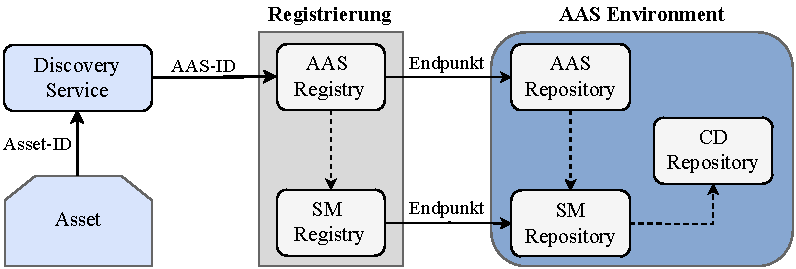
\includegraphics[width=1\textwidth]{Bilder/Ergebnisse/Systemarchitektur/BaSyx.pdf}
    \caption{BaSyx-Backend}
    \label{fig:BaSyxArchitektur}
\end{figure}

Der Discovery Service übernimmt die Auflösung einer Asset-ID (globalAssetId) in die zugehörige \acs{aas}-ID und ermöglicht so das gezielte Auffinden einer \acs{aas} im Gesamtsystem. 
Die Registries dienen als Verzeichnisse aller registrierten \acs{aas} und Submodelle einschließlich ihrer Endpunkte innerhalb der \acs{aas} Environment, wobei die \acs{aas} Registry optional auch Referenzen auf die Submodel Registry (SM Registry) enthalten kann. 

Die \acs{aas} Environment selbst beherbergt die eigentlichen Inhalte und ist in drei Repositories gegliedert. 
Das AAS Repository verwaltet die \acs{aas} einschließlich Asset-Metadaten und Referenzen auf Submodelle. 
Das Submodel Repository (SM Repository) speichert die Submodelle mit ihren jeweiligen Inhalten und Referenzen auf die zugehörigen Concept Descriptions. 
Diese werden im \acs{cd} Repository verwaltet und beeinhalten alle semantischen Beschreibungen.

Alle Komponenten verfügen dabei über eine standardisierte REST-API, die sowohl anderen Systemen als auch den Komponenten selbst einen einheitlichen Zugriff auf ihre Inhalte ermöglicht. 
Zudem sind sie an eine gemeinsame MongoDB angebunden, in der sämtliche Daten persistent gespeichert werden.

Die dynamische Erweiterung ergänzt die Kernarchitektur um die Fähigkeit zur Verarbeitung von Echtzeit- und Zeitreihendaten. 
Abbildung~\ref{fig:DynamischeErweiterungArchitektur} zeigt den Aufbau der zusätzlichen Komponenten sowie deren Zusammenspiel mit dem bestehenden System.

Der Datengenerator und der Maschinensimulator simulieren die robocell-Maschine und erzeugen sowohl Zustands- als auch kontinuierlich Prozessdaten. 
Beide Anwendungen stellen ihre Daten über einen OPC UA Server bereit und sind über die Databridge direkt an die AAS Environment im BaSyx-Backend angebunden.
Zusätzlich werden die vom Datengenerator simulierten Werte mithilfe von Telegraf kontinuierlich in eine InfluxDB geschrieben, wodurch eine historische Datenbasis entsteht. 

\begin{figure}[htbp]
    \centering
        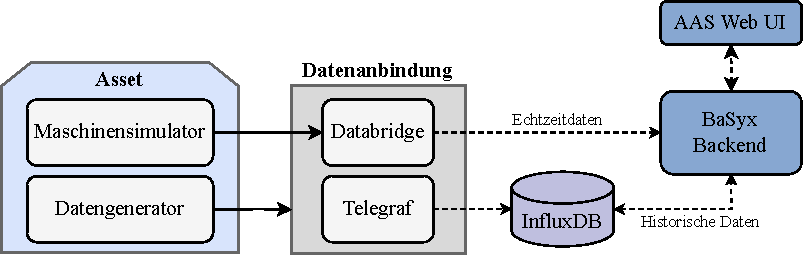
\includegraphics[width=1\textwidth]{Bilder/Ergebnisse/Systemarchitektur/DynamischeErwweiterung.pdf}
    \caption{BaSyx Backend}
    \label{fig:DynamischeErweiterungArchitektur}
\end{figure}

Zur Weiterverarbeitung und Visualisierung, sowohl der statischen Inhalte der AAS als auch der durch die dynamische Erweiterung ergänzten Echtzeit- und Zeitreihendaten, kommt die AAS Web UI zum Einsatz. 
Alternativ könnten auch benutzerdefinierte Anwendungen verwendet werden, die beispielsweise zusätzliche Analysen ermöglichen oder spezifische Anforderungen erfüllen.

Die AAS Web UI greift über die standardisierten Schnittstellen der Komponenten des zuvor vorgestellten BaSyx-Backends auf die Registrierungsdaten der AAS sowie deren Submodelle und Inhalte zu. 
Statische Daten und Echtzeitdaten werden dabei direkt aus dem Submodel Repository abgefragt. 
Bei Zeitreihendaten hingegen ist nicht der eigentliche Dateninhalt in der AAS gespeichert, sondern lediglich ein Verweis auf den zugehörigen Endpunkt in der InfluxDB hinterlegt. 
Die AAS Web UI nutzt diesen Endpunkt, um die historischen Daten direkt aus der Datenbank abzurufen und in der Web-Oberfläche zu visualisieren.

\subsubsection{Statische Submodelle}
Die statische Modellierung des Demonstrators erfolgte im Package Explorer.
Dazu wurden alle relevanten AAS sowie die zugehörigen Submodelle angelegt, mit Inhalten befüllt, semantisch angereichert und mit eindeutigen Identifikatoren versehen.
Als Hauptdatenquellen dienten die technischen Dokumentationen der robocell, insbesondere die Betriebsanleitung, sowie Informationen aus dem PLM-System Agile.

Abbildung~\ref{fig:PackageExplorerRobocell} zeigt die Gesamtübersicht des Abfüll- und Verschließmoduls. 
Die statischen Submodelle sind darin mit einer Nummer gekennzeichnet, die der im Folgenden verwendeten Gliederung entspricht. 
Sie beinhalten feststehende, beschreibende Inhalte, die nicht zur Laufzeit geändert werden. 
Zur besseren Veranschaulichung wird das Submodell BOM ausführlicher beschrieben.
Die grundlegende Struktur der weiteren statischen Submodelle ist im Anhang~\ref{sec:AnhangSubmodelle} ergänzend anhand von Screenshots dokumentiert.

\begin{figure}[htbp]
    \centering
        \includegraphics[width=1\textwidth]{Bilder/ErgebnissePackageExplorer/AASrobocellTestAuflösung.PNG}
    \caption{Package Explorer: Gesamtübersicht AAS-Demonstrator}
    \label{fig:PackageExplorerRobocell}
\end{figure}

\subsubsection*{1) Typenschild}
\vspace{-0.5em} 
Das Submodell Typenschild bildet die zentrale Identifikationsstelle der Maschine innerhalb der AAS. 
Es erfasst grundlegende Angaben wie Hersteller, Seriennummer, Produkttyp oder Softwareversionen. 
Funktional entspricht es einem physischen Typenschild, erweitert dieses jedoch um maschinenlesbare und interoperable Inhalte. 
Darüber hinaus bietet es den Vorteil, dass auch zusätzliche Dateien wie Zertifikate oder Logos direkt eingebunden werden können.

\subsubsection*{2) Technische Daten}
\vspace{-0.5em}

Das Submodell Technische Daten dient als technisches Datenblatt der Maschine.  
Es gliedert sich in die Bereiche Allgemeine Informationen sowie Technische Eigenschaften. 
Letztere sind in mehreren \acsp{smc} organisiert, beispielsweise für Produktionsmedien, Umgebungsbedingungen, elektrische Daten oder den Verarbeitungsbereich. 
Die einzelnen \acsp{smc} enthalten überwiegend Properties oder Ranges, die Parameter wie etwa elektrische Kenndaten beschreiben. 
Auf diese Weise sind alle relevanten technischen Angaben an einem zentralen Ort gebündelt, was der redundanten Pflege in verschiedenen Systemen oder Dokumenten entgegenwirkt. 

\subsubsection*{3) BOM}
\vspace{-0.5em}

Das BOM-Submodell dient dazu, die Maschinenstruktur sichtbar zu machen und die Beziehungen zwischen ihren einzelnen Komponenten hierarchisch abzubilden, vergleichbar mit einer digitalen Stückliste.
Dabei enthält es verschiedene Entitäten, die jeweils eine untergeordnete Komponente repräsentieren.
Die Beziehungen zwischen den Komponenten werden über Relationship-Elemente mit einer eindeutigen semanticId gemäß dem \acs{smt} Hierarchical Structures enabling Bills of Material \cite{SpezifikationHierachischeStrukturen} hergestellt.

Zur Veranschaulichung wurde die Grundmaschine als Beispiel gewählt, da sie weniger komplex als die Maschinenebene ist, aber dennoch alle relevanten Strukturelemente enthält.
Abbildung~\ref{fig:BOMSubmodelGrundmashcine} zeigt das entsprechende Submodell, in dem weitere untergeordnete Komponenten aufgeführt sind, darunter auch das Bedientableau.
Dieses ist als Self-Managed Entity angelegt und über die globalAssetId mit seiner AAS verknüpft (Abbildung~\ref{fig:AASBedientableau}), die wiederum ein eigenes BOM-Submodell mit weiteren Unterkomponenten enthält.

\begin{figure}[htbp]
    \centering
        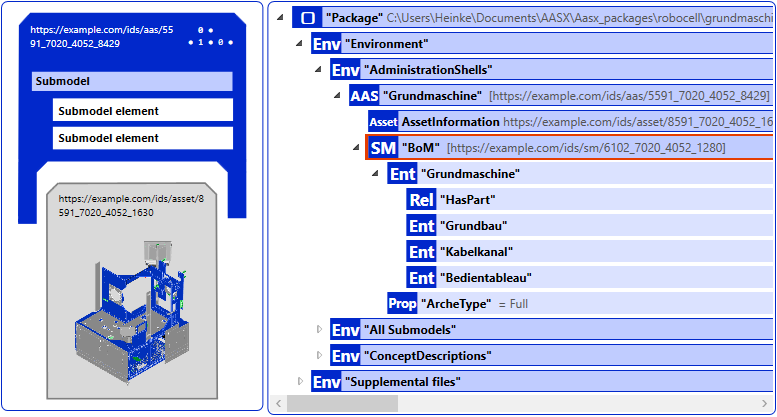
\includegraphics[width=1\textwidth]{Bilder/ErgebnissePackageExplorer/AASGrundmaschine.PNG}
    \caption{Package Explorer: BOM-Submodell der Grundmaschine}
    \label{fig:BOMSubmodelGrundmashcine}
\end{figure}

\begin{figure}[htbp]
    \centering
        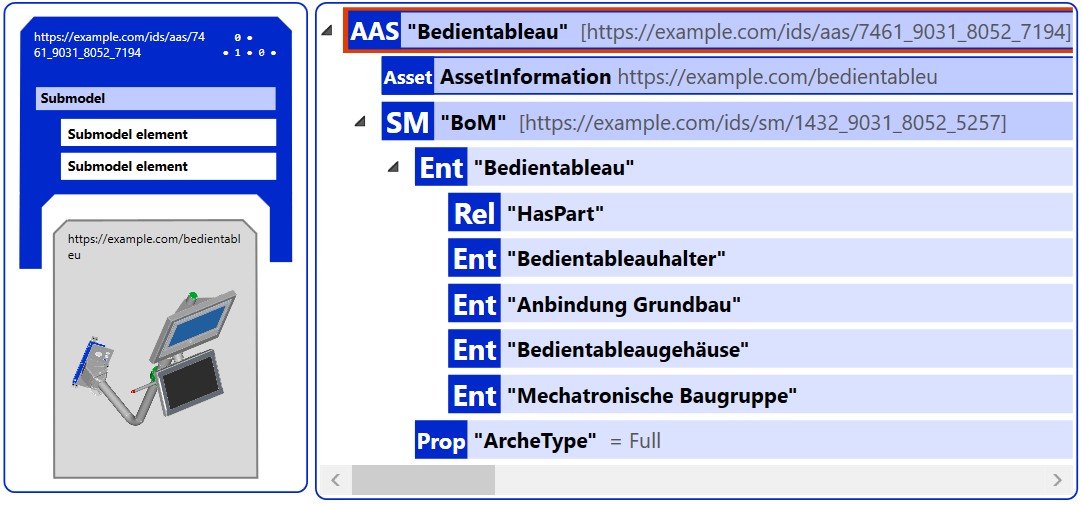
\includegraphics[width=1\textwidth]{Bilder/ErgebnissePackageExplorer/BedientableauTest.PNG}
    \caption{Package Explorer: AAS des Bedientableaus}
    \label{fig:AASBedientableau}
\end{figure}


Mit diesem Prinzip lässt sich die gesamte Maschine rekursiv abbilden. 
Jede Komponente wird als eigenständige AAS geführt und ist somit unabhängig von der übergeordneten Struktur wiederverwendbar. 
Dies ermöglicht eine modulare und herstellerübergreifende Integration, da auch externe Komponenten eingebunden werden können.

\subsubsection*{4), 5) Dokumentation und 3D-Modelle}
\vspace{-0.5em}

Beide Submodelle dienen der Bereitstellung und Klassifizierung zentraler Maschinendateien. 
Das Submodell Dokumentation umfasst technische Unterlagen wie die Betriebsanleitung oder die Netzwerkübersicht, während das Submodell 3D-Modelle CAD-Daten zur Geometrie beeinhaltet. 
Alle Dateien sind als File-Elemente direkt in die Struktur der AAS eingebettet und jeweils in eigenen \acsp{smc} organisiert, die zusätzlich Metainformationen zu Identifikation, Klassifikation und Versionierung enthalten. 
Das Submodell 3D-Modelle könnte darüber hinaus um weitere Metadaten, etwa zu Darstellungsoptionen oder Geometrieinformationen, ergänzt werden, was im Demonstrator jedoch nicht umgesetzt wurde. 
Dadurch ermöglichen beide Submodelle nicht nur das Einbetten von Dateien, sondern auch deren eindeutige Beschreibung und Rückverfolgbarkeit über den gesamten Lebenszyklus hinweg.

\subsubsection*{6) Wartung}
Das Submodell Wartung bildet den digitalen Wartungsplan der Maschine ab. 
Für jede wartungsrelevante Komponente sind in eigenen \acsp{smc} letzte Wartungszeitpunkte, Intervalle, zuständige Personen oder Organisationen sowie die vorgesehenen Maßnahmen hinterlegt. 
Es ermöglicht damit die strukturierte Verwaltung sowohl bereits durchgeführter als auch anstehender Wartungen und gewährleistet eine nachvollziehbare Dokumentation. 
Darüber hinaus schafft das Submodell die Grundlage für eine dynamische Erweiterung. 
So könnte beispielsweise ein Betriebsstundenzähler angebunden werden, der automatisch Wartungsbedarf erkennt, oder es könnte in Kombination mit Predictive-Maintenance-Ansätzen genutzt werden, um auf Basis von Sensordaten proaktiv Wartungsmaßnahmen abzuleiten und diese direkt in der AAS darzustellen. 

\textbf{Zusammenfassung}  

Die statischen Submodelle bündeln alle relevanten Stammdaten der Maschine zentral an einem Ort. 
Dadurch wird eine einfache Weitergabe der Informationen entlang der Wertschöpfungskette ermöglicht. 
So kann die AAS beispielsweise in Form einer AASX-Datei an einen Betreiber übergeben werden, der direkten Zugriff auf die Daten benötigt. 
Ebenso können AAS einzelner Komponenten nahtlos in den digitalen Zwilling der Gesamtmaschine integriert werden. 
Durch die Orientierung an standardisierten \acsp{smt} und die semantische Beschreibung sind die Inhalte zudem interoperabel und können von unterschiedlichen Systemen oder Personen gleichermaßen interpretiert und genutzt werden. 

\subsubsection{Dynamische Submodelle}
\label{sec:DynamischeSubmodelle}
Neben den statischen Submodellen wurden im Demonstrator auch dynamische Submodelle umgesetzt.
Sie ermöglichen die kontinuierliche Erfassung und Aktualisierung von Maschinen- und Prozessdaten sowie die Interaktion mit dem zugrunde liegenden Asset.
Da im Rahmen dieser Arbeit keine reale Maschine zur Verfügung stand, wird dieses Asset durch den Datengenerator und den Maschinensimulator repräsentiert.

Die technische Umsetzung und die zugrunde liegenden Datenflüsse orientieren sich an etablierten Industriearchitekturen, sodass die Schnittstellen und Funktionsweisen ohne Anpassungen auch mit einem realen System genutzt werden könnten.
Durch diese Erweiterung erfüllt der Demonstrator die Anforderungen an einen digitalen Zwilling gemäß der in Kapitel~\ref{sec: DT} beschriebenen Klassifizierung.

\subsubsection*{Prozessdaten}

Das Submodell Prozessdaten dient der Erfassung und Bereitstellung zentraler Betriebsinformationen.
Im Rahmen dieser Arbeit wurden exemplarisch die Messgrößen Füllstand, Durchfluss, Anzahl abgefüllter Einheiten und Druck implementiert.
Die Werte stammen aus dem \acs{opcua}-Server des Datengenerators, der sie im Sekundentakt aktualisiert und über die Databridge nahezu in Echtzeit an die \acs{aas} überträgt.
Vor der Speicherung im Submodel Repository erfolgt eine zweistufige Transformation.
Zunächst werden die Rohdaten mithilfe des Jackson-Transformers in ein JSON-Format überführt, anschließend extrahiert JSONata die relevanten Messgrößen, die schließlich den entsprechenden Properties des Submodells zugeordnet werden.

\begin{figure}[htbp]
    \centering
    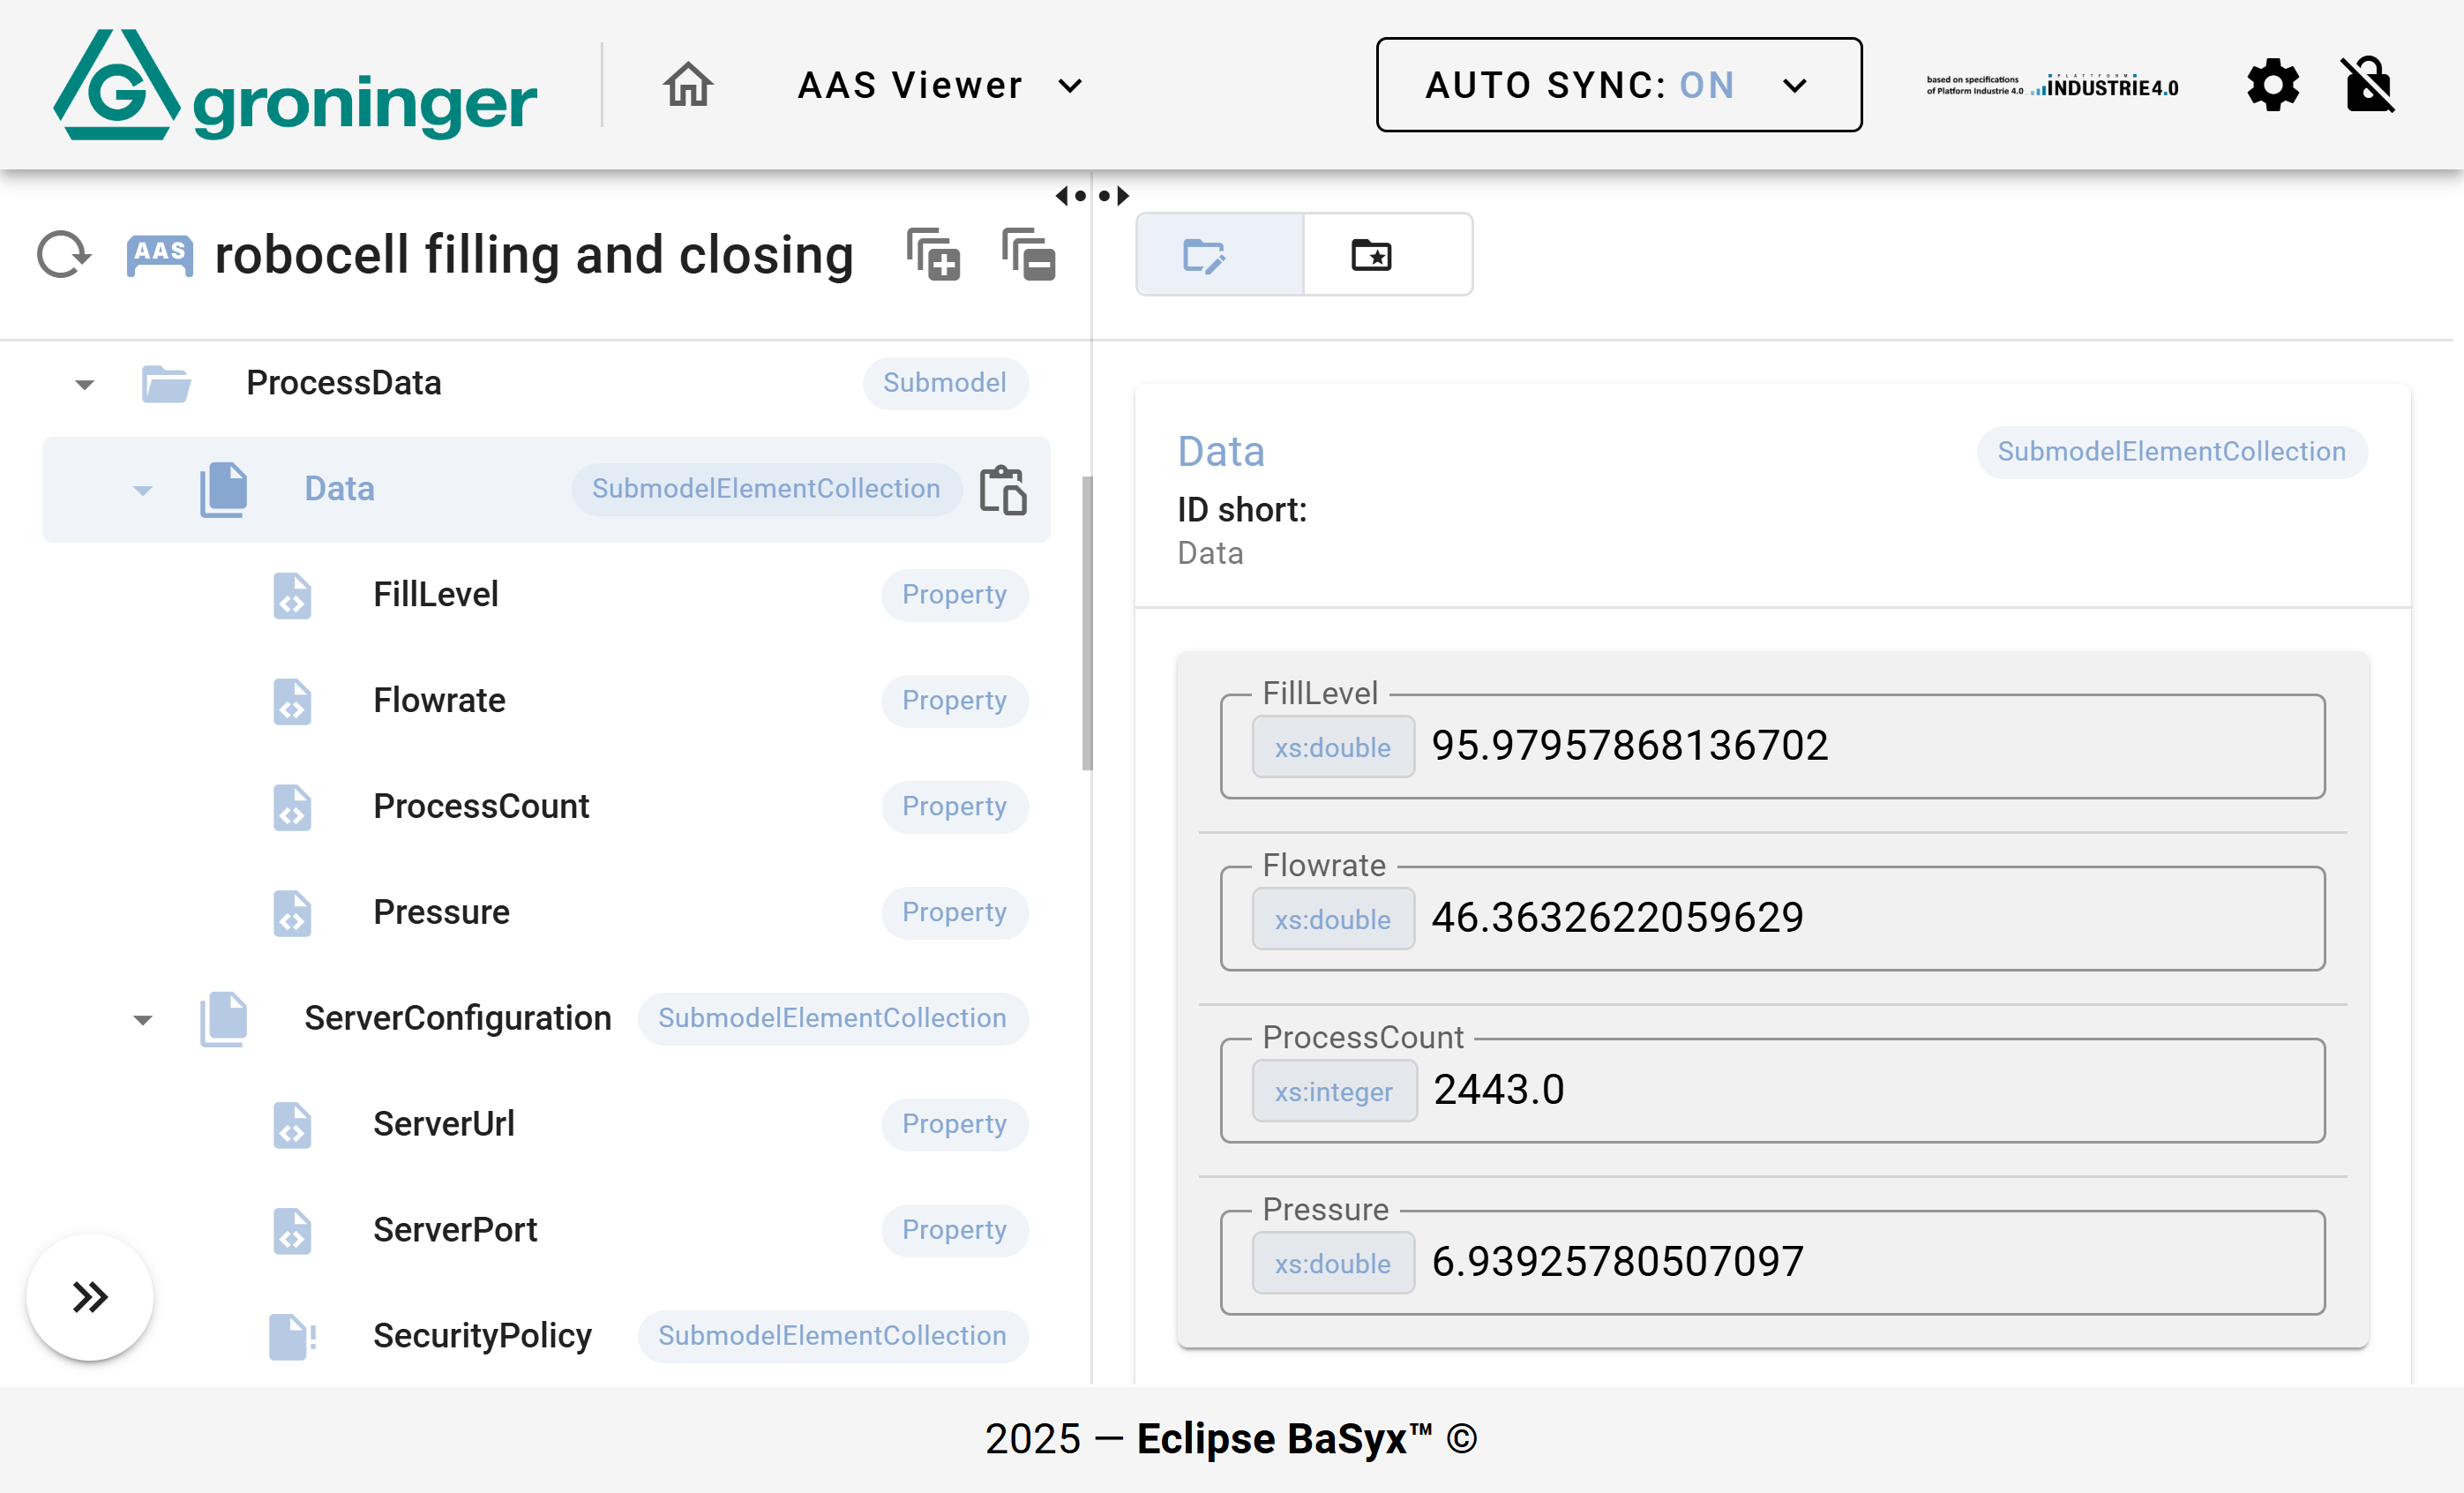
\includegraphics[width=1\textwidth]{Bilder/ErgebnisseAASWebUI/ProcessData.png}
    \caption{AAS Web UI: Prozessdaten}
    \label{fig:Processdata}
\end{figure}
\vspace{-0.5em}

Die Visualisierung der Prozessdaten erfolgt in der klassischen Elemente-Ansicht der AAS Web UI, wie in Abbildung~\ref{fig:Processdata} dargestellt, oder über ein speziell entwickeltes Plugin.
Damit die Werte in der Benutzeroberfläche aktuell bleiben, kann eine Synchronisationsfunktion aktiviert werden.
Dabei ruft die Weboberfläche die relevanten Daten in festen Intervallen, beispielsweise alle vier Sekunden, automatisch vom Repository ab.

Die Umsetzung ist protokolloffen und könnte grundsätzlich auf weitere Kommunikationsstandards wie \acs{mqtt} oder \acs{rest} erweitert werden.
Eine automatische bidirektionale Kommunikation, etwa das Zurückschreiben von Werten aus der \acs{aas} in externe Systeme, ist mit der eingesetzten Databridge derzeit jedoch nicht möglich.

\subsubsection*{Kontrollkomponente}
Das Submodell Kontrollkomponente dient der Abbildung und Visualisierung des aktuellen Maschinenstatus sowie der unterstützten Betriebsmodi.
Die Zustandsinformationen stammen aus dem Maschinensimulator, der sie in numerischer Form über einen \acs{opcua}-Server bereitstellt.
Über die Databridge werden diese Werte in nahezu Echtzeit in die \acs{aas} übertragen.
Vor der Speicherung erfolgt eine semantische Umwandlung mithilfe von JSONata, um die numerischen Codes in sprechende Zustandsbezeichnungen zu überführen.

Die Zustände orientieren sich am PackML-Standard (Packaging Machine Language), einem von der OMAC (Organization for Machine Automation and Control) entwickelten Modell zur einheitlichen Beschreibung von Maschinenzuständen und zulässigen Zustandsübergängen, insbesondere für Verpackungsmaschinen \cite{OMAC}. 
Der Standard definiert insgesamt 17 Maschinenzustände und legt fest, welche Übergänge zwischen diesen möglich sind. 
Dieses Konzept kommt auch bei der robocell-Linie zum Einsatz und ermöglicht eine konsistente und interoperable Erfassung des Maschinenstatus über verschiedene Systeme hinweg.

Die Visualisierung erfolgt über ein in die AAS Web UI integriertes Vue.js-Plugin, das den Maschinenstatus als PackML-Zustandsautomat darstellt.
Das Plugin basiert auf einer Entwicklung der Hochschule für Technik und Wirtschaft Berlin \cite{HTW1, HTW2} und wurde funktional angepasst, um es in die AAS Web UI zu integrieren und die im Demonstrator benötigten Steuer- und Anzeigeoptionen zu unterstützen.

Abbildung~\ref{fig:PackMLZustandsautomat} zeigt die Darstellung des Zustandsautomaten in der Benutzeroberfläche.
Damit Statusänderungen unmittelbar sichtbar werden, ist eine Polling-Logik implementiert, die den aktuellen Maschinenstatus in festen Intervallen aus dem Submodel Repository der AAS Environment abruft und im Zustandsautomaten aktualisiert.

Neben der reinen Statusanzeige erlaubt das Plugin auch die Steuerung zulässiger Zustandsübergänge direkt aus der Benutzeroberfläche heraus.
Befindet sich die Maschine beispielsweise im Zustand Execute, können Befehle wie Stop, Hold, Suspend oder Abort ausgelöst werden.
Darüber hinaus lässt sich der Betriebsmodus (Produktion, Manuell oder Wartung) setzen, der ebenfalls als Property im Submodell verwaltet wird.

\newpage
\begin{figure}[htbp]
    \centering 
    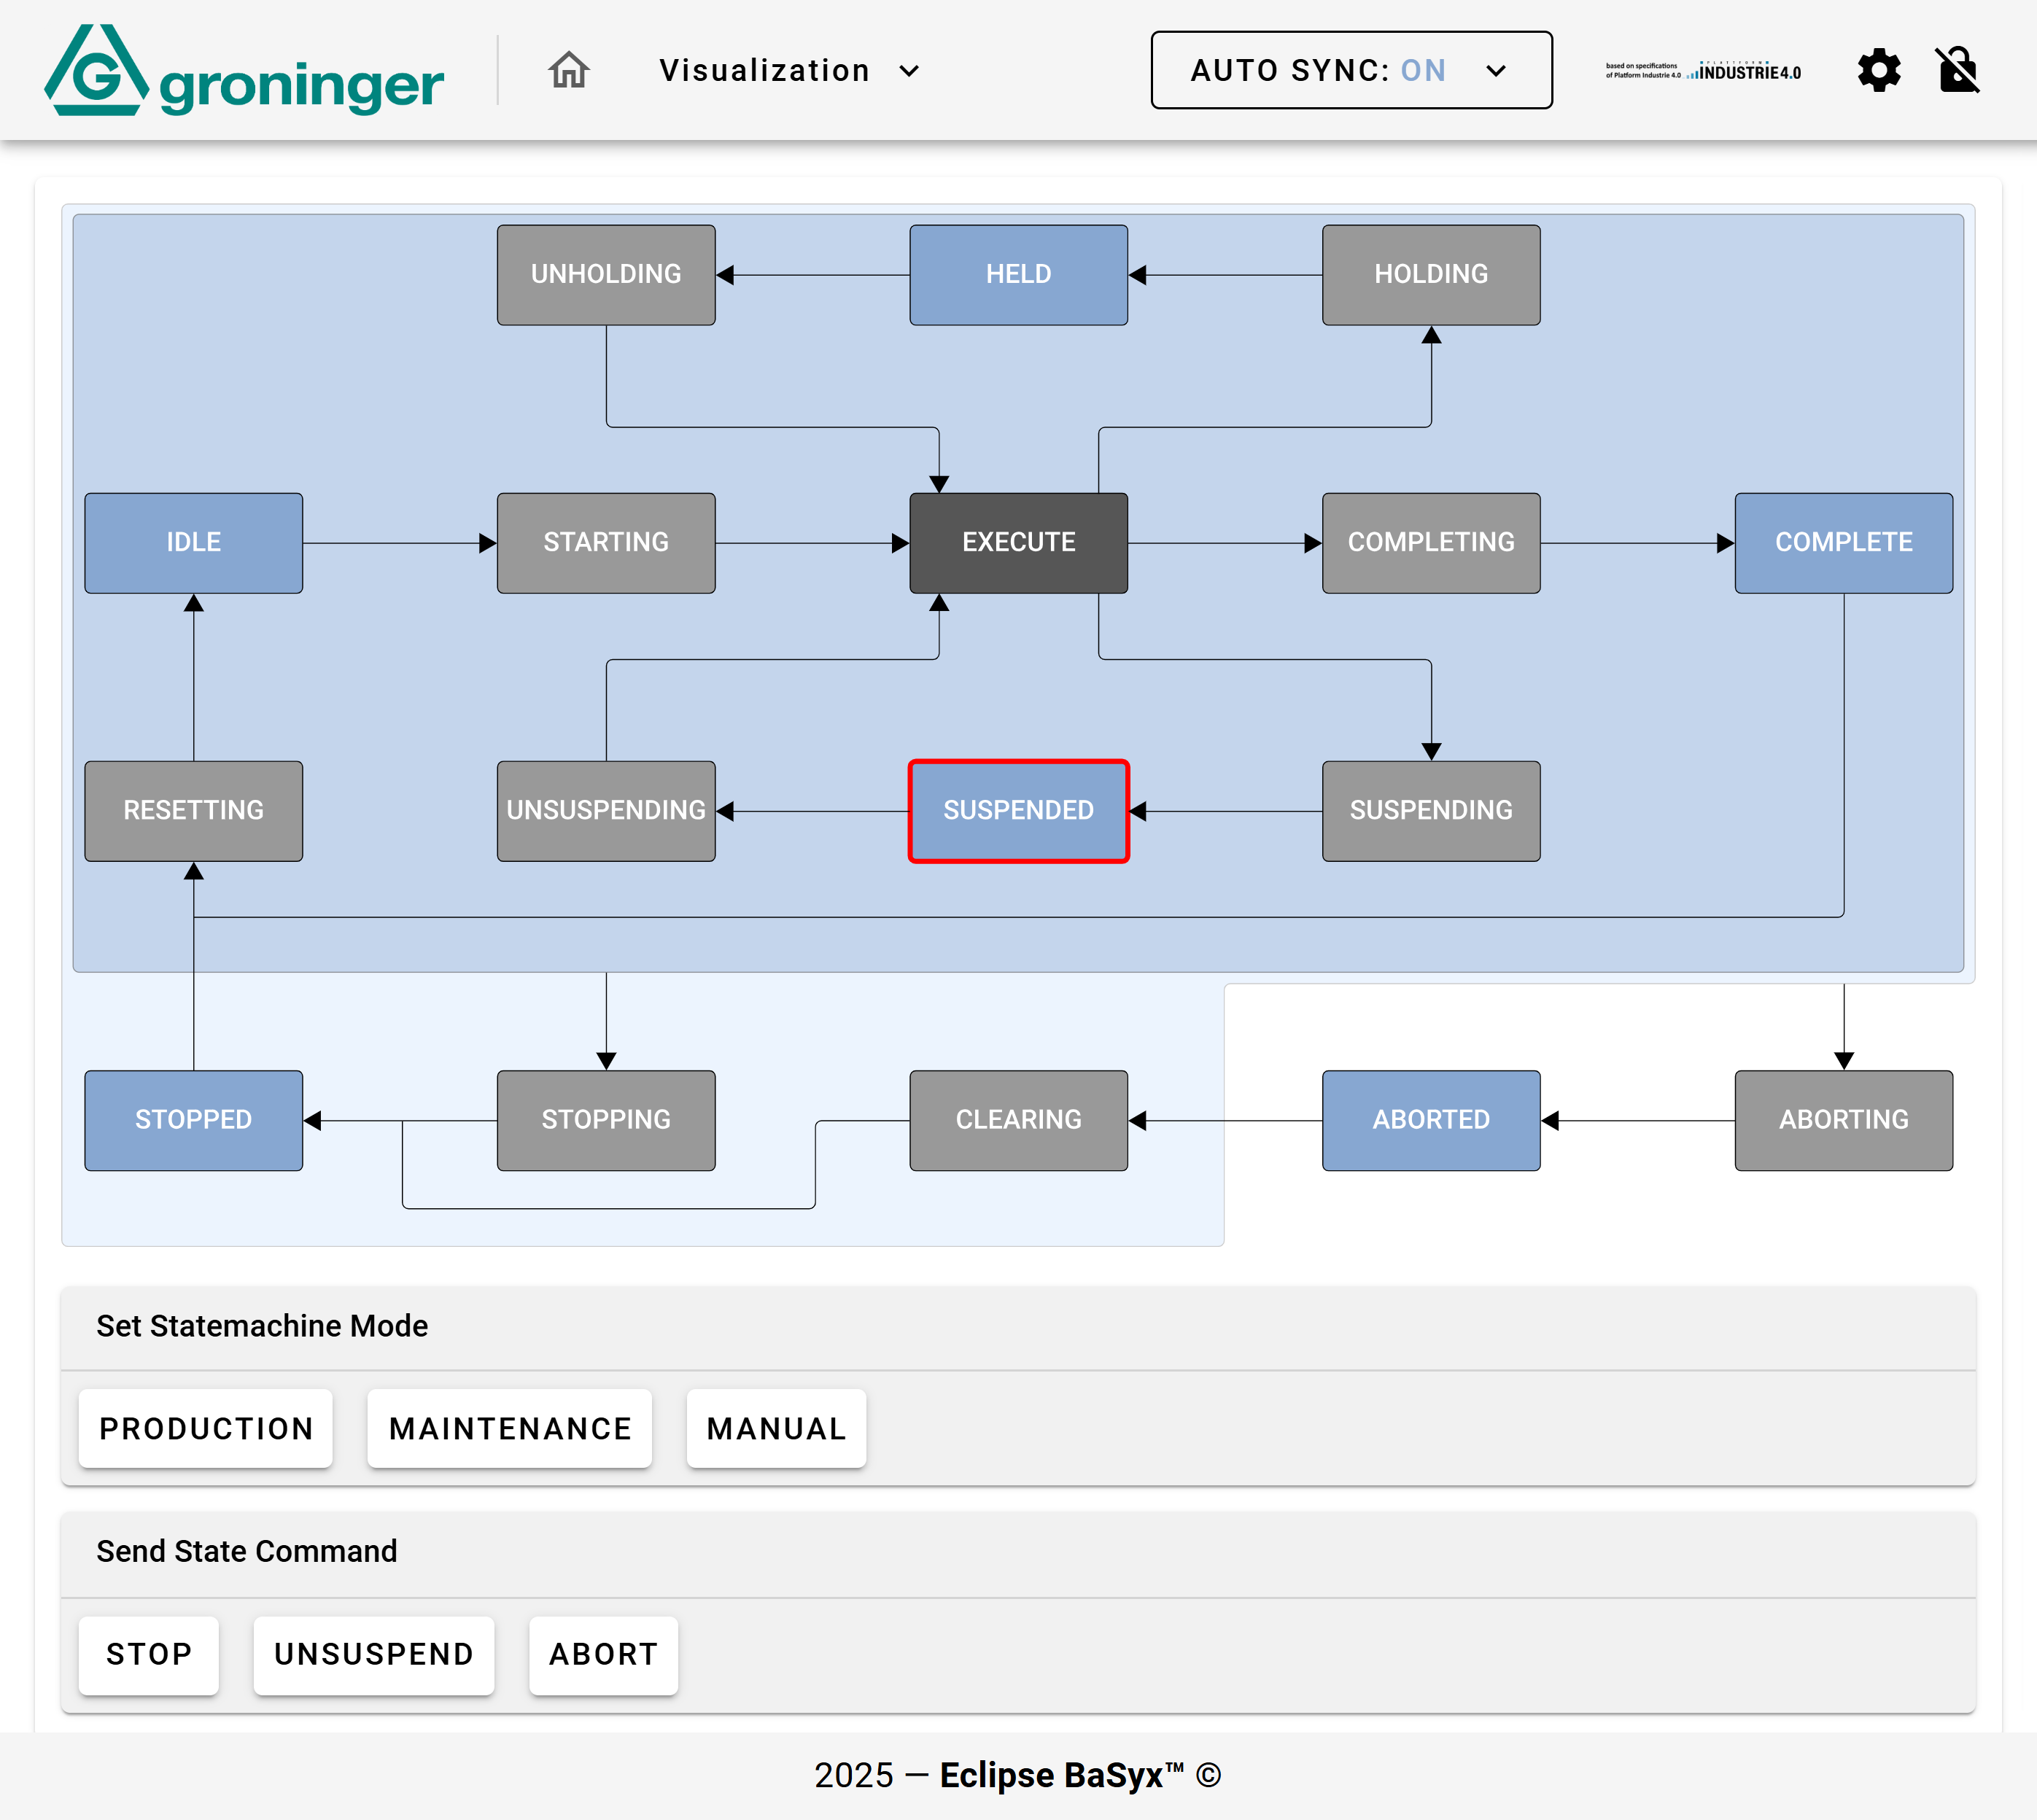
\includegraphics[width=1\textwidth]{Bilder/ErgebnisseAASWebUI/Kontrollkomponente.png} 
    \caption{AAS Web UI: PackML-Zustandsautomat} 
    \label{fig:PackMLZustandsautomat} 
\end{figure}
\vspace{-0.5em}

Im Demonstrator werden Befehle direkt per WebSocket an den Maschinensimulator übermittelt und dort ohne weitere Prüfungen übernommen. 
Dadurch entsteht eine direkte Feedback-Schleife zwischen der \acs{aas} und dem simulierten Asset.
In einer realen Maschine würden diese Signale hingegen zunächst über ein geeignetes Industrieprotokoll wie \acs{opcua} an die speicherprogrammierbare Steuerung (SPS) übertragen und dort validiert werden müssen, bevor der neue Zustand an die \acs{aas} zurückgemeldet wird.

\subsubsection*{Zeitreihendaten}
Das Submodell Zeitreihendaten dient der Einbettung historischer Messwerte in die \acs{aas}. 
Im Demonstrator werden hierfür exemplarisch die Messgrößen Druck und Temperatur verwendet, die kontinuierlich vom \acs{opcua}-Server des Datengenerators bereitgestellt werden. 
Anstatt diese Werte direkt in der \acs{aas} abzulegen, werden sie mithilfe von Telegraf in die externe InfluxDB-Datenbank übertragen. 
Telegraf abonniert dazu die relevanten Variablen des \acs{opcua}-Servers und schreibt geänderte Werte unmittelbar in die Datenbank.

Die Anbindung an die \acs{aas} erfolgt über ein LinkedSegment (eine \acs{smc}) im Submodell, das alle für die Datenabfrage erforderlichen Parameter enthält, wie den Endpunkt der InfluxDB und die zugehörige Abfragebeschreibung. 
Dadurch können Anwendungen, die auf die \acs{aas} zugreifen, die Zeitreihendaten gezielt abrufen, ohne Details zur technischen Implementierung der Datenbank kennen zu müssen.

Zur Visualisierung steht in der AAS Web UI ein spezielles Plugin zur Verfügung, das auf die im LinkedSegment hinterlegten Parametern zugreift und Abfragen an die InfluxDB stellt. 
Ein Nutzer kann dabei auswählen, ob einzelne Messgrößen oder kombinierte Ansichten mehrerer Werte angezeigt werden sollen. 
Abbildung~\ref{fig:LiniendiagrammBaSyx} zeigt exemplarisch ein Liniendiagramm mit den zeitlichen Verläufen von Druck und Temperatur über einen Zeitraum von fünf Minuten.

\begin{figure}[htbp]
    \centering
        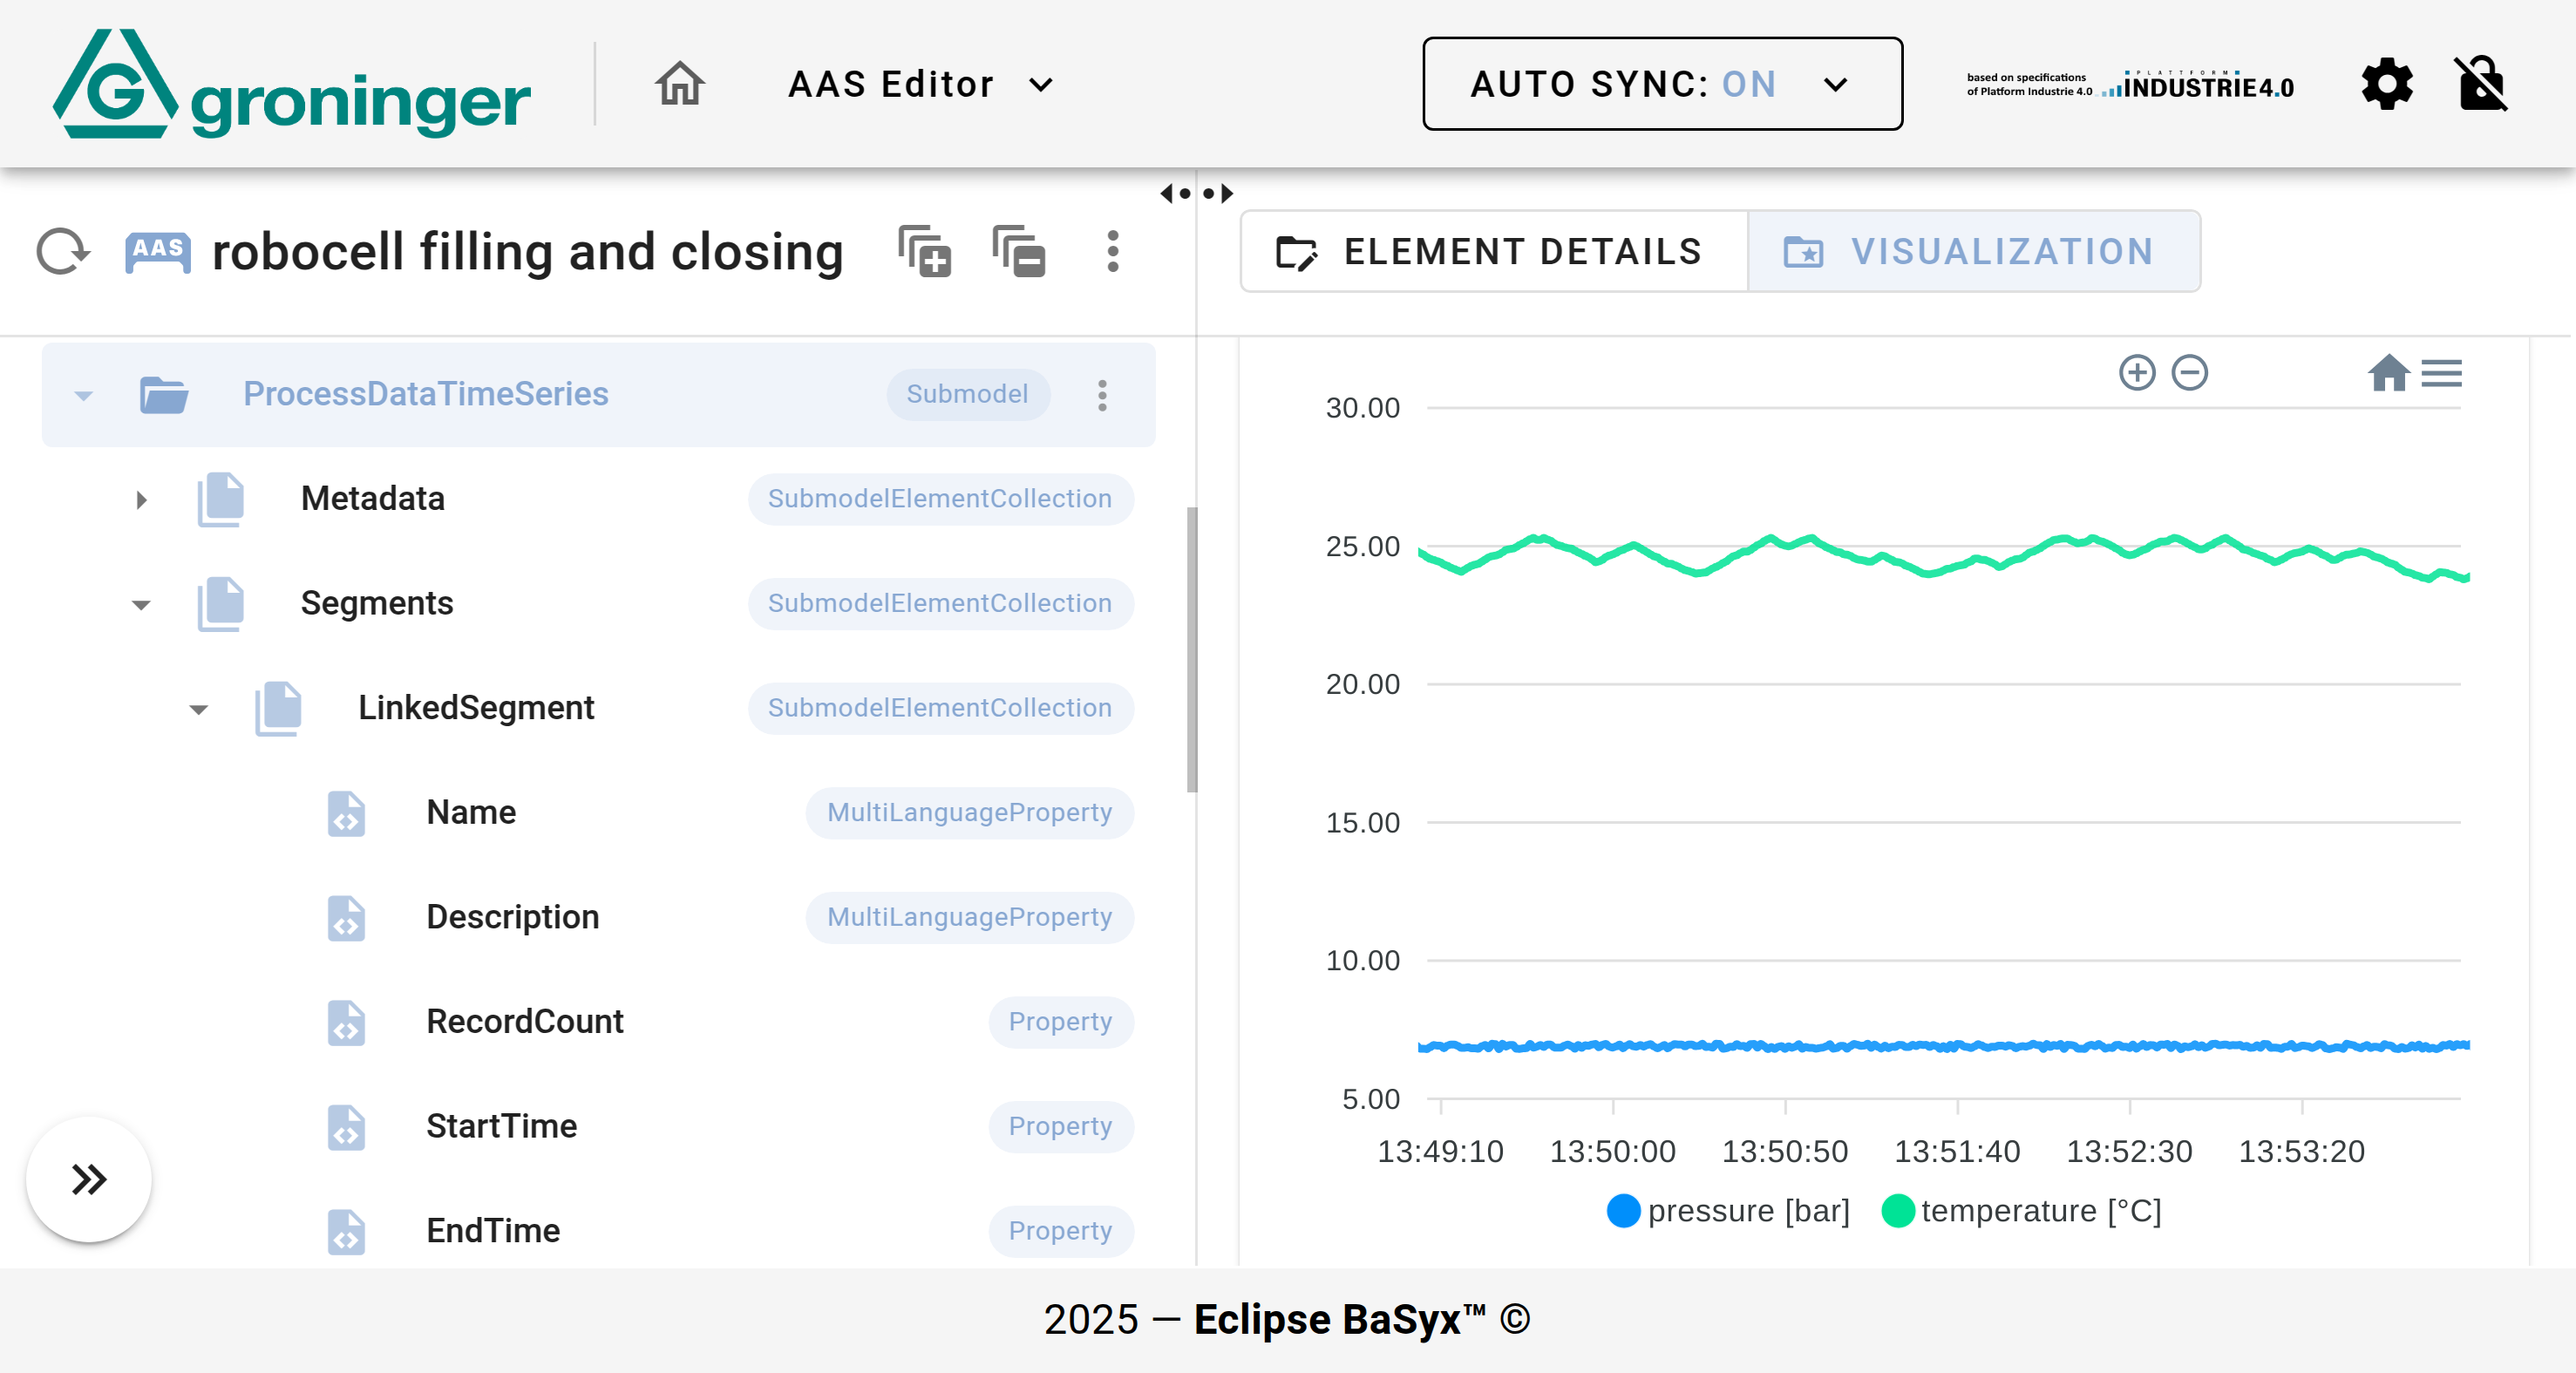
\includegraphics[width=1\textwidth]{Bilder/ErgebnisseAASWebUI/Zeitreihen.png}
    \caption{AAS Web UI: Zeitreihendaten (Liniendiagramm)}
    \label{fig:LiniendiagrammBaSyx}
\end{figure}
\vspace{-0.5em}

Ein wesentlicher Vorteil dieser Umsetzung liegt in der Entkopplung von Datenspeicherung und \acs{aas}. 
Da die \acs{aas} selbst nicht für die Ablage großer oder historischer Datenmengen ausgelegt ist, ermöglicht die Auslagerung in eine externe Zeitreihendatenbank eine effiziente Speicherung und Verarbeitung. 
Zudem können die Daten durch die strukturierte Referenzierung über das LinkedSegment einfach in weiteren Anwendungen, wie Analysesystemen oder KI-gestützten Verfahren, weiterverwendet werden.

\subsubsection{Herausforderungen bei der Implementierung}
Im Rahmen der Implementierung des Demonstrators traten verschiedene Herausforderungen auf, die sowohl technische als auch methodische Aspekte betrafen. 
Diese ergaben sich unter anderem aus der noch jungen Verbreitung der \acs{aas} im Maschinenbau, der eingeschränkten Datenverfügbarkeit sowie den Limitierungen der eingesetzten Werkzeuge. 
Die wesentlichen Punkte sind im Folgenden zusammengefasst:

\begin{enumerate}
    \item \textbf{Fehlende praxisnahe Vorlagen für den Maschinenbau:}  
    Zwar existieren bereits diverse \acsp{smt}, Spezifikationen sowie allgemeine Anwendungsfälle, diese sind jedoch primär auf Komponentenhersteller ausgerichtet.  
    Konkrete Vorlagen und praxisnahe Anwendungsfälle, die speziell auf den Maschinenbau und die Anforderungen des Demonstrators zugeschnitten sind, standen jedoch nur begrenzt zur Verfügung.

    \item \textbf{Begrenzte Datenverfügbarkeit:}  
    Da keine reale Maschine angebunden war, mussten Echtzeitdaten simuliert werden.  
    Zudem waren nicht alle relevanten Daten im PLM-System so dokumentiert, dass eine direkte Übernahme möglich gewesen wäre.  
    Viele Informationen mussten daher manuell aus verschiedenen Dokumenten, wie der Betriebsanleitung, extrahiert werden.  

    \item \textbf{Begrenzte Verfügbarkeit semantischer Beschreibungen:}  
    Für viele spezifische Maschineneigenschaften, wie technische Parameter im Verarbeitungsbereich (z.\,B. Spritze, Vial, Zylinderampulle) und deren Detailwerte (z.\,B. Füllmenge, Stopfenhöhe), existieren bislang keine standardisierten ECLASS-Beschreibungen.  
    Diese mussten daher manuell angelegt werden, was zeitaufwendig war und die Interoperabilität einschränkt.

    \item \textbf{Eingeschränkte Funktionalität der eingesetzten Tools:}  
    Die verwendeten Werkzeuge unterstützten nicht alle benötigten Funktionen.  
    So wurden beispielsweise beim Hochladen von Dateien in der AAS Web UI keine Einträge im Discovery Service erzeugt.  
    Da diese Funktionalität erforderlich war, musste sie mithilfe eines eigens entwickelten Skripts ergänzt werden.  
    Eine detaillierte Evaluierung der eingesetzten Tools erfolgt in Kapitel~XY.

    \item \textbf{Inkonsistenzen zwischen Spezifikationen und Tools:}  
    \acsp{smt} und die zugehörigen Spezifikationen wiesen teilweise Inkonsistenzen auf, etwa unterschiedliche Werte in der Dokumentation im Vergleich zu den AASX-Vorlagen.  
    Dies führte dazu, dass einige Plugins nicht oder nur eingeschränkt funktionierten, da sie auf korrekte semantische Beschreibungen angewiesen sind.  
    Die Fehlerbehebung erforderte eine manuelle Anpassung der \acsp{smt}, was zusätzlichen Aufwand verursachte.
\end{enumerate}

\newpage
\subsection{KI-Modell zur Anomalieerkennung}

Für die Anomalieerkennung wurde der zuvor trainierte Autoencoder im Evaluierungsmodus eingesetzt, sodass während der Auswertung keine Anpassungen der Modellparameter erfolgen.
Die Testdaten basieren, wie beim Training, auf simulierten Temperaturverläufen aus dem Datengenerator, die analog zu den Zeitreihendaten in Kapitel \ref{sec:DynamischeSubmodelle} in einer InfluxDB gespeichert wurden.

Als Eingabe erhält das Modell kurze Sequenzen von jeweils fünf Messwerten.
Im Unterschied zur Trainingsphase enthalten die Testdaten gezielt eingefügte Anomalien, um die Erkennungsfähigkeit des Modells zu prüfen.
Dabei wurden vier Anomalietypen simuliert: dauerhaft erhöhte Werte, ein einzelner ausgeprägter Peak, ein linearer Anstieg über mehrere Zeitpunkte sowie invertierte Werte im Vergleich zum Normalverlauf.

Während der Auswertung berechnet der Autoencoder für jede Sequenz den Rekonstruktionsfehler als durchschnittliche Abweichung zwischen Eingabe- und Ausgabedaten. 
Zur Klassifikation dient ein Schwellenwert, der aus dem Mittelwert des Fehlers plus dem Zweifachen der Standardabweichung gebildet wird. 
Überschreitet der Fehler einer Sequenz diesen Wert, wird das gesamte Zeitfenster als Anomalie markiert.

Zur Veranschaulichung werden zwei Beispiele gezeigt, die unterschiedliche Anomalietypen repräsentieren. 
Abbildung~\ref{fig:Fall1} zeigt einen Temperaturverlauf mit dauerhaft erhöhten Werten im Bereich t = 10000 - 10010 (gezielt eingefügte Anomalie). 
Das Modell erkennt die Anomalie zuverlässig, allerdings leicht verzögert. 
Dies liegt an der Mittelwertbildung über das Fünf-Werte-Fenster.
Erst wenn mehrere aufeinanderfolgende Werte vom Normalverlauf abweichen, steigt der Fehler ausreichend an.

\begin{figure}[htbp]
    \centering
        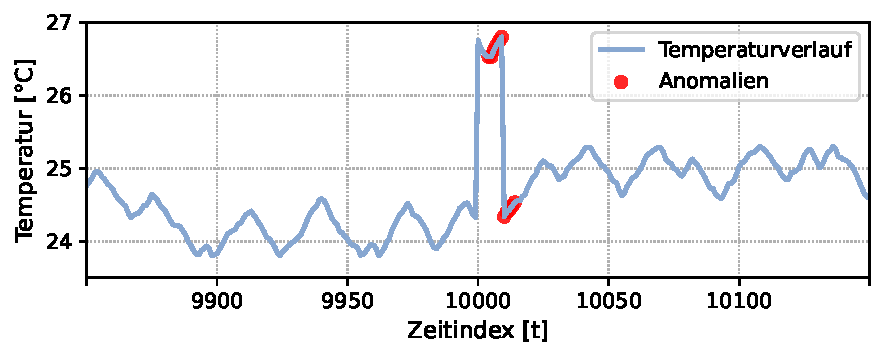
\includegraphics[width=1\textwidth]{Bilder/Ergebnisse/KI/Fall1.pdf}
        \vspace{-2em}
    \caption{Anomalieerkennung Fall 1: Überhöhte Daten}
    \label{fig:Fall1}
\end{figure}
\vspace{-0.5em}

In Abbildung~\ref{fig:Fall2} ist ein Temperaturverlauf mit einem gleichmäßigen, linearen Anstieg im Bereich t = 25343 - 25393 (gezielt eingefügte Anomalie) dargestellt. 
Auch hier klassifiziert das Modell den Verlauf korrekt als Anomalie. 
Dies zeigt, dass die Erkennung nicht nur auf plötzliche Ausreißer reagiert, sondern auch schleichende Veränderungen im Signalverlauf erkennt.


\begin{figure}[htbp]
    \centering
        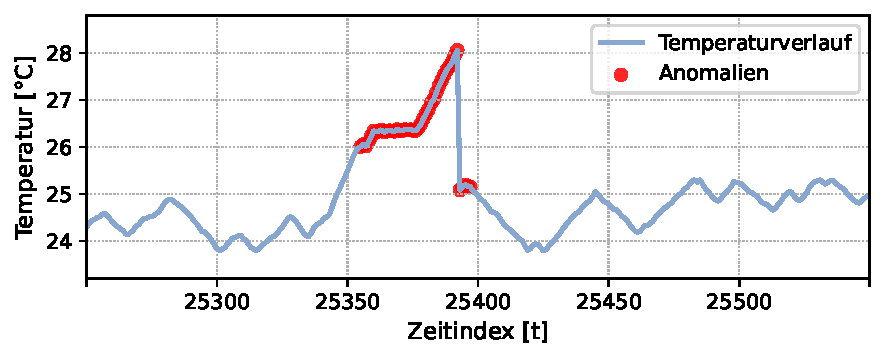
\includegraphics[width=1\textwidth]{Bilder/Ergebnisse/KI/Fall2.pdf}
        \vspace{-2em}
    \caption{Anomalieerkennung Fall 2: Linearer Anstieg}
    \label{fig:Fall2}
\end{figure}
\vspace{-0.5em}

In allen Testfällen mit künstlich erzeugten Anomalien erfolgte die Klassifikation korrekt, ohne Fehlalarme. 
Aufgrund der Fenstergröße und der Mittelwertbildung tritt die Markierung jedoch häufig leicht verzögert auf, wodurch einzelne Sequenzen innerhalb einer Anomaliephase nicht als abweichend markiert werden. 
Da ausschließlich synthetische Abweichungen geprüft wurden, ist zu erwarten, dass reale Anomalien aufgrund ihrer höheren Komplexität eine größere Herausforderung darstellen.

Zur Verbesserung könnten umfangreichere und variantenreichere Trainings- und Testdaten eingesetzt werden. 
Auch leistungsfähigere Architekturen wie tiefere Autoencoder oder LSTM-basierte Netze (Long Short-Term Memory, eine spezielle Form rekurrenter neuronaler Netze zur Verarbeitung von Zeitreihen) bieten Potenzial, zeitliche Abhängigkeiten präziser zu erfassen.
Diese Ansätze wurden aufgrund begrenzter Rechenressourcen im Rahmen dieser Arbeit nicht weiterverfolgt, können aber eine Grundlage für zukünftige Entwicklungen bilden.

Dennoch zeigt sich, dass das gewählte Konzept grundsätzlich umsetzbar ist und sich für eine Einbettung in industrielle Szenarien eignet. 
In Verbindung mit realen Maschinendaten könnten erkannte Anomalien genutzt werden, um proaktive Wartungsmaßnahmen einzuleiten. 
Dadurch ließe sich die Anlagenverfügbarkeit erhöhen und ungeplante Stillstandszeiten verringern.
Werden neben Sensordaten zusätzlich technische Stammdaten oder standardisierte Beschreibungen berücksichtigt, wie sie auch im AAS-Demonstrator hinterlegt sind, wird eine noch umfassendere Analyse möglich, die zugleich die Grundlage für weiterführende Predictive-Maintenance-Ansätze bilden könnte.

\newpage
\subsection{Anwendungsfall Digitaler Produktpass}
Der Anwendungsfall Digitaler Produktpass demonstriert, wie Nachhaltigkeitsinformationen in Form von \acs{pcf}-Werten direkt in der AAS einer Maschine abgebildet werden können.
Grundlage bildet der in Kapitel \ref{sec:AAS-Demonstrator} vorgestellte AAS-Demonstrator, der zu diesem Zweck um ein Submodell zur Abbildung des \acs{cf} erweitert wurde.
Neben der dynamischen Berechnung und Aggregation dieser Werte wird im Folgenden auch dargestellt, wie der Zugriff auf die im DPP enthaltenen Informationen durch unterschiedliche Nutzerrollen und technische Clients geregelt ist.

\subsubsection{Abbildung des PCF}
Das CF-Submodell bildet die Lebenszyklusphasen Material, Produktion und Cradle to Gate jeweils in eigenen \acsp{smc} ab.
Abbildung~\ref{fig:SubmodellCF} zeigt exemplarisch die \acs{smc} für die Phase Cradle to Gate (links) sowie die integrierte Komponentenliste (rechts), in der die für die Berechnung herangezogenen Siemens-Komponenten hinterlegt sind.

\begin{figure}[htbp]
    \centering
        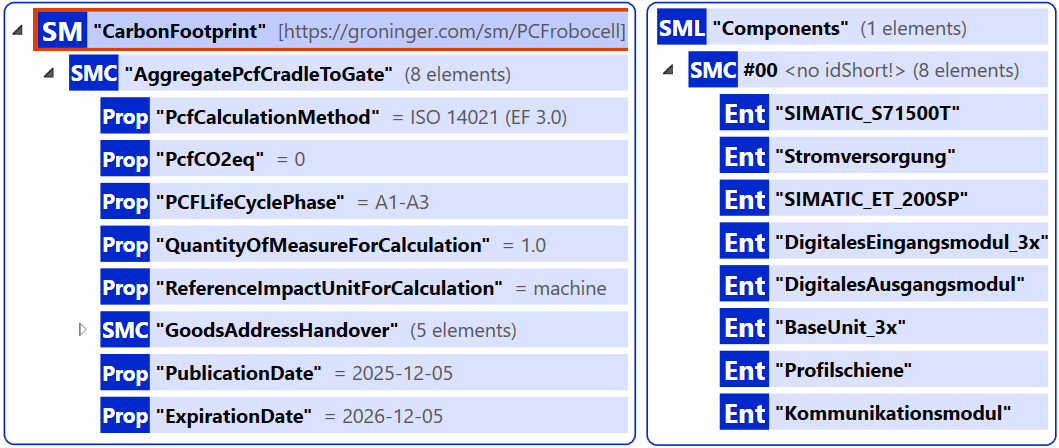
\includegraphics[width=1\textwidth]{Bilder/ErgebnissePackageExplorer/CarbonFoorprintTest.png}
    \caption{CF-Submodell der robocell}
    \label{fig:SubmodellCF}
\end{figure}

Die Aggregation der CO\textsubscript{2}-Äquivalente erfolgt dynamisch über einen Microservice. 
Dieser ist als Docker-Container implementiert und greift über die REST-Schnittstellen des BaSyx-Backends auf die in der Komponentenliste hinterlegten Entitäten zu. 
Mithilfe des Discovery Service werden deren AAS identifiziert und vorhandene CF-Submodelle ausgelesen. 
Die enthaltenen PCF-Werte werden anschließend zu Gesamtwerten für die einzelnen Lebenszyklusphasen aggregiert und in das CF-Submodell der Haupt-AAS zurückgeschrieben.

Die Berechnung kann direkt über ein Plugin in der AAS Web UI ausgelöst werden.
 Nach Abschluss des Berechnungsprozesses werden die aktualisierten Werte automatisch vom Submodel Repository abgefragt und in der Benutzeroberfläche aktualisiert.
Abbildung~\ref{fig:PluginAggregation} zeigt die entsprechende Visualisierung: links die aggregierten CO\textsubscript{2}-Äquivalente, rechts die zugehörigen Lebenszyklusphasen.

\begin{figure}[htbp]
    \centering
        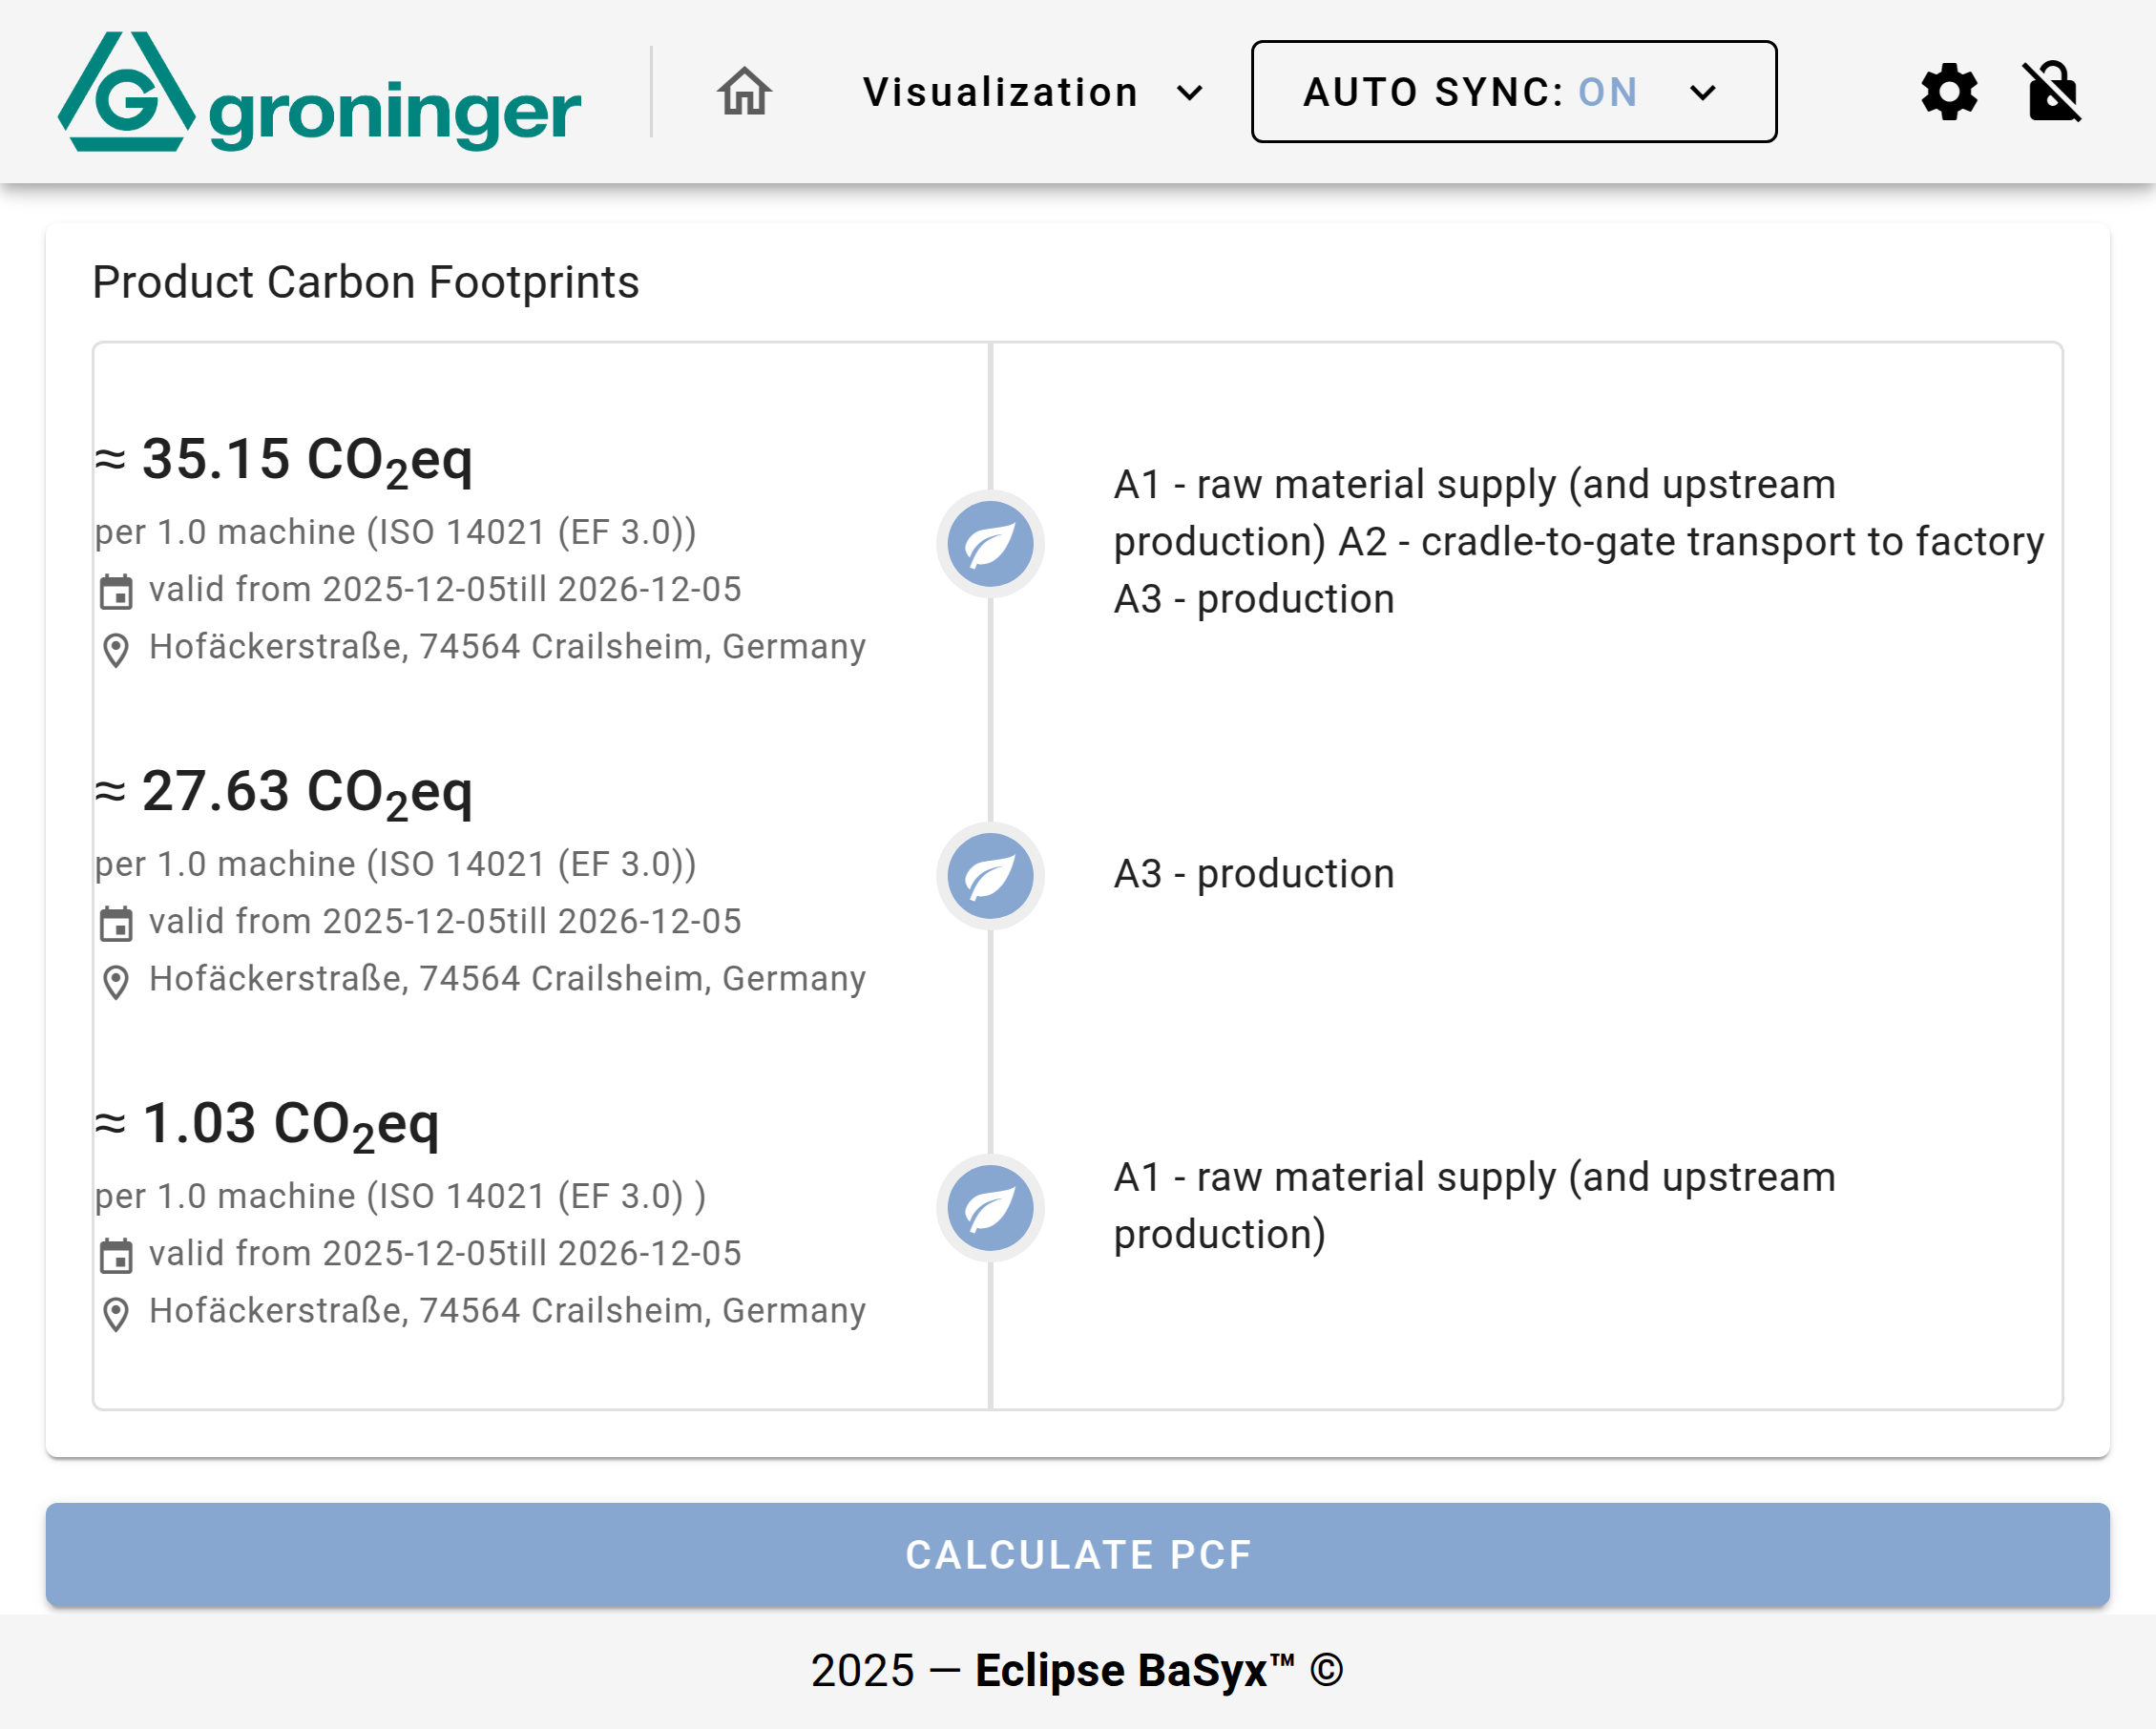
\includegraphics[width=1\textwidth]{Bilder/ErgebnisseAASWebUI/CarbonFootprint.png}
    \caption{Visualisierung der aggregierten PCF-Werte}
    \label{fig:PluginAggregation}
\end{figure}

Der Ansatz ist flexibel erweiterbar.
Bei Verfügbarkeit weiterer Komponenten-AAS lässt sich die Liste unkompliziert ergänzen, sodass sukzessive die gesamte Maschine berücksichtigt werden kann. 
Perspektivisch ist auch eine Erweiterung auf weitere Lebenszyklusphasen, wie Nutzung oder Entsorgung, sowie die Einbeziehung des TCF denkbar, um eine ganzheitliche ökologische Bilanzierung zu ermöglichen.

\subsubsection{Rollenbasierter Zugriff auf Submodelle}
Der digitale Produktpass wird im Demonstrator durch die erweiterte AAS der robocell-Maschine repräsentiert. 
Um sensible Inhalte gezielt und sicher bereitzustellen, wurde eine rollenbasierte Zugriffskontrolle implementiert. 
Die Authentifizierung und Autorisierung erfolgt über Keycloak, das als Docker-Container in die BaSyx-Architektur integriert ist.

Exemplarisch wurden drei Nutzer mit zugehörigen Rollen eingerichtet, deren Rechte in separaten Konfigurationsdateien für die jeweiligen BaSyx-Dienste hinterlegt sind.

\newpage
\begin{itemize}[noitemsep, leftmargin=*, label=\textbullet]
  \item \makebox[6cm][l]{\textbf{groninger.meyer}} (Rolle: \textit{Groninger-Mitarbeiter})
    \begin{itemize}[noitemsep, leftmargin=2em, label=--]
      \item uneingeschränkter Zugriff auf alle Submodelle
    \end{itemize}
  \item \makebox[6cm][l]{\textbf{customer.doe}} (Rolle: \textit{Kunde})
    \begin{itemize}[noitemsep, leftmargin=2em, label=--]
      \item Zugriff auf ausgewählte Submodelle (z.\,B. Typenschild, CF)
    \end{itemize}
  \item \makebox[6cm][l]{\textbf{technician.john}} (Rolle: \textit{Service-Techniker})
    \begin{itemize}[noitemsep, leftmargin=2em, label=--]
      \item Lese- und Schreibrechte auf wartungsrelevante Submodelle
    \end{itemize}
\end{itemize}
\vspace{0.5em}

Eine Möglichkeit zur Einsicht der im \acs{dpp} enthaltenen Informationen bietet die AAS Web UI.
Ist \acs{rbac} aktiviert, wird der Benutzer beim Aufruf der Oberfläche automatisch zur Keycloak-Anmeldeseite weitergeleitet.
Wie in Abbildung~\ref{fig:KeycloakAnmeldeSeite} dargestellt, erfolgt die Authentifizierung über die in Keycloak hinterlegten Zugangsdaten.

\begin{figure}[htbp]
    \centering
        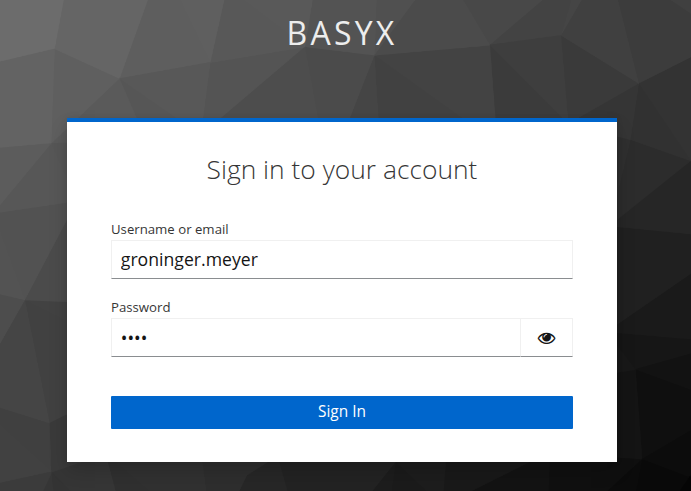
\includegraphics[width=0.7\textwidth]{Bilder/Ergebnisse/DPP/KeycloakAnmeldeSeite.png}
    \caption{Keycloak-Anmeldeseite für die AAS Web UI}
    \label{fig:KeycloakAnmeldeSeite}
\end{figure}

Nach erfolgreicher Anmeldung erhält die AAS Web UI ein Zugriffstoken mit den Rolleninformationen des Nutzers.
Dieses Token wird bei allen Anfragen an die BaSyx-Komponenten automatisch mitgesendet.
Die jeweiligen Dienste prüfen es gegen die hinterlegten \acs{rbac}-Regeln und entscheiden so über die tatsächliche Zugriffsberechtigung.

Meldet sich beispielsweise der Nutzer customer.doe an, so sieht er nur die für seine Rolle freigegebenen Submodelle. 
Andere Submodelle wie Kontrollkomponente oder Wartung bleiben verborgen. 
Zudem besitzt er ausschließlich Leserechte, das heißt Änderungsversuche werden mit einem Fehler abgelehnt.

Neben der AAS Web UI ist auch ein direkter Zugriff auf die BaSyx-Komponenten über die REST-API möglich, der insbesondere für technische Clients relevant ist. 
Dafür wurden in Keycloak drei Clients mit Service Accounts angelegt, die denselben Rollen wie die Benutzerkonten entsprechen und somit identische Berechtigungen besitzen.

Zur Validierung der Konfiguration wurde Postman eingesetzt. 
Die Clients rufen dabei über den Token-Endpunkt von Keycloak Zugriffstokens ab und nutzen diese für API-Anfragen. 
Abbildung~\ref{fig:KeycloakAnmeldeSeite} zeigt exemplarisch eine DELETE-Anfrage des Service-Techniker-Clients. 
Da dieser nur Leserechte besitzt, wird die Anfrage mit HTTP 403 Forbidden abgelehnt. 
Mit dem Groninger-Client hingegen gelingt der Löschvorgang, da dessen Rolle uneingeschränkte Rechte umfasst (HTTP 204 No Content).

\begin{figure}[htbp]
    \centering
        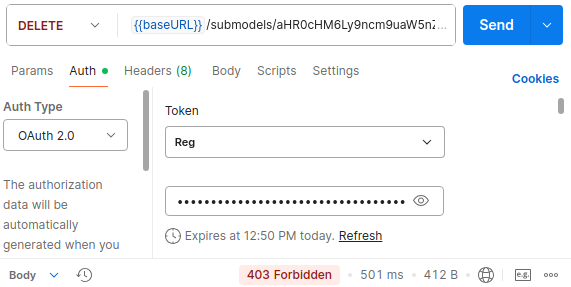
\includegraphics{Bilder/Ergebnisse/DPP/Postman/TechnicianDelet.png}
    \caption{DELETE-Anfrage des Service-Techniker-Clients in Postman}
    \label{fig:KeycloakAnmeldeSeite}
\end{figure}

Die Zugriffskontrolle mit BaSyx und Keycloak zeigt, dass sich Berechtigungen zuverlässig auf die AAS und ihre Submodelle übertragen lassen.
Dies bestätigt die Eignung der AAS als technische Grundlage für den \acs{dpp} und eröffnet Potenziale für Szenarien, in denen sensible Informationen, etwa Nachhaltigkeitsdaten, differenziert entlang der Wertschöpfungskette bereitgestellt werden.

\subsection{Anwendungsfall automatisierte Generierung von AAS}
Dieser Anwendungsfall demonstriert, wie sich AAS-Instanzen automatisiert erzeugen und in das BaSyx-System integrieren lassen.
Abbildung \ref{fig:AutomatisierteGenerierungAblauf} veranschaulicht den Ablauf.
Ausgangspunkt bildet ein unternehmensspezifisches Typ-Submodell, das mithilfe des Package Explorers aus dem SMT Generic Frame for Technical Data for Industrial Equipment in Manufacturing \cite{SpezifikaitonTechnischeDaten} abgeleitet wurde.
Dieses Template wird anschließend über ein Node.js-basiertes Mapping-Skript mit Beispieldaten ergänzt und in eine neue AAS-Instanz eingebettet.
Das Skript übernimmt auch die Registrierung im BaSyx-Backend, sodass die erzeugte AAS unmittelbar zur Verfügung steht und beispielsweise in der AAS Web UI visualisiert werden kann.

\begin{figure}[htbp]
    \centering
        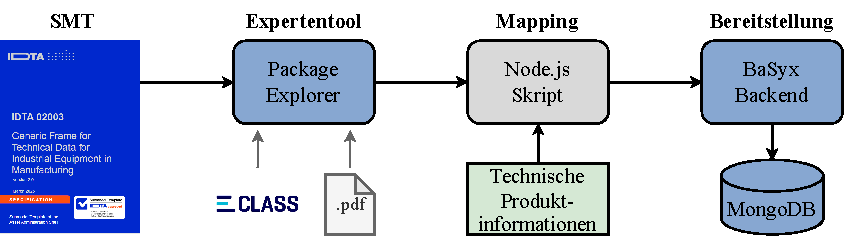
\includegraphics{Bilder/ErgebnisseAutomatisierteGenerierung/ARchitektur.pdf}
    \caption[Ablauf der automatisierten Generierung einer AAS]{Ablauf der automatisierten Generierung einer AAS (eigene Darstellung; Bildbestandteile: \cite{SpezifikaitonTechnischeDaten}, \cite{ECLASSLogo} )}
    \label{fig:AutomatisierteGenerierungAblauf}
\end{figure}

Der entwickelte Ansatz verdeutlicht, dass sich der manuelle Modellierungsaufwand im Package Explorer durch den teilautomatisierten Prozess erheblich reduzieren lässt. 
In diesem Anwendungsfall wurden zwar statische Beispieldaten eingesetzt, in einer produktiven Umgebung könnten jedoch die technischen Produktinformationen direkt aus bestehenden IT-Systemen übernommen werden. 
Bei groninger stammen diese primär aus dem PLM-System Agile. 
Eine entsprechende Anbindung war im Rahmen dieser Arbeit jedoch nicht umsetzbar.

Darüber hinaus ist der Prozess grundsätzlich auch auf weitere Submodelle übertragbar, sodass perspektivisch die AAS einer gesamten Maschine automatisiert erstellt werden könnte. 
Zudem wäre es möglich, die Mapping-Logik in eine Laufzeitumgebung zu integrieren. 
Dadurch ließe sich die Generierung, Bereitstellung und Aktualisierung von AAS-Instanzen vollständig automatisieren.

%Evaluation der eingesetzten Software
\subsection{Evaluierung eingesetzter Tools und Software}
Zur Umsetzung des AAS-Demonstrators sowie der zugehörigen Anwendungsfälle kamen zwei zentrale Softwarelösungen zum Einsatz.
Im Folgenden werden diese mit Blick auf ihre Funktionalität sowie ihre Stärken und Schwächen evaluiert.
Die Bewertung stützt sich dabei auf die Erfahrungen aus der praktischen Anwendung und berücksichtigt sowohl technische Aspekte als auch die Benutzerfreundlichkeit.

\subsubsection{Package Explorer}

Der Package Explorer wurde während der gesamten Projektlaufzeit als zentrales Modellierungstool eingesetzt.
Er ermöglichte die Erstellung, Bearbeitung und Visualisierung von AAS einschließlich ihrer Submodelle und Submodellelemente.
Besonders hilfreich war die Möglichkeit, semantische Beschreibungen direkt aus ECLASS-Katalogen zu importieren.
Dadurch verringerte sich der ansonsten sehr aufwendige manuelle Aufbau eigener Concept Descriptions deutlich, was den Modellierungsprozess spürbar beschleunigte.
Zudem überzeugte die benutzerfreundliche Oberfläche, die den Einstieg erleichterte, das Verständnis der AAS-Strukturen förderte und Verstöße gegen die Spezifikation der IDTA unmittelbar kenntlich machte.

In der praktischen Anwendung zeigten sich jedoch auch Einschränkungen.
Die integrierte Validierungsfunktion erwies sich als unzuverlässig, sodass zur Absicherung eine separate Test-Engine erforderlich war.
Während die Anbindung an den AASX Server Blazor problemlos funktionierte, war eine direkte Integration in modulare Laufzeitsysteme wie Eclipse BaSyx nicht möglich.
Die AAS mussten daher manuell bereitgestellt werden, was insbesondere bei einer größeren Anzahl oder häufigen Änderungen mit erheblichem Mehraufwand verbunden war.
Darüber hinaus wich der Package Explorer in einzelnen Punkten von den aktuellen AAS-Spezifikationen ab, was vereinzelt zu fehlerhaften semantischen Angaben führte, die nachträglich korrigiert werden mussten.

Insgesamt erwies sich der Package Explorer als hilfreiches Werkzeug für die statische Modellierung von AAS.
Die vorhandenen Exportfunktionen, insbesondere im AASX-Format, erleichterten die Weiterverwendung und Weitergabe maßgeblich.
Für automatisierte Szenarien bot das Tool hingegen nur eingeschränkte Unterstützung, die sich im Wesentlichen auf das Anlegen eigener \acsp{smt} beschränkte.

\subsubsection{Eclipse BaSyx}

Die Eclipse-BaSyx-Plattform bildete in diesem Projekt die zentrale Laufzeitumgebung für den Betrieb von \acs{aas}.
Ein wesentlicher Vorteil war der modulare Aufbau, der die Umsetzung praxisnaher Industrieszenarien erlaubte und zugleich eine flexible Konfiguration einzelner Komponenten zuließ.
Ebenso eröffneten die standardisierten REST-APIs einen direkten Zugriff auf die einzelnen Komponenten, der dank der integrierten Swagger-Dokumentation unmittelbar getestet und transparent nachvollzogen werden konnte.
Darüber hinaus erleichterte die DataBridge die Anbindung unterschiedlicher Protokolle, insbesondere von OPC UA, wodurch eine dynamische Erweiterung der AAS und die Umsetzung dynamischer Submodelle möglich wurde.

Mit der AAS Web UI stand zudem eine Benutzeroberfläche zur Verfügung, die sowohl die Darstellung als auch die Anpassung von AAS-Inhalten erlaubte. 
Für zentrale Submodelle waren bereits spezialisierte Plugins vorhanden, die sich aufgrund des Open-Source-Charakters leicht erweitern oder durch eigene Entwicklungen ergänzen ließen.
Auf diese Weise konnten weitere Submodelle integriert und projektspezifische Anforderungen berücksichtigt werden.
Als besonders hilfreich erwies sich zudem die Synchronisationsfunktion, die insbesondere in dynamischen Szenarien sicherstellte, dass die angezeigten Daten stets aktuell blieben.

Aufgrund der Komplexität des Gesamtsystems war jedoch ein erheblicher Konfigurationsaufwand erforderlich.
Dies betraf nicht nur die initiale Einrichtung, sondern zeigte sich auch bei der Konfiguration der rollenbasierten Zugriffskontrolle (\acs{rbac}), die für jede Komponente separat vorgenommen werden musste.
Hinzu kam, dass der Start des Systems in der Docker-Umgebung vergleichsweise lange dauerte, da einzelne Komponenten teilweise bis zu mehreren Minuten für den Startvorgang benötigten.
Dies erwies sich insbesondere bei häufigen Anpassungen oder Testläufen als hinderlich.

Darüber hinaus zeigte sich, dass die Plattform in einzelnen Bereichen noch nicht vollständig ausgereift ist.
So war es beispielsweise beim Ändern von Werten innerhalb einer Property über die REST-API nur möglich, String-Werte einzutragen, auch wenn ein anderer Datentyp, wie etwa ein Integer, vorgesehen war.
Zudem erfolgte beim Ablegen aktualisierter \acs{aas} in das gemountete Volume der AAS Environment nicht immer eine zuverlässige Synchronisierung der zugehörigen Concept Descriptions.
In diesen Fällen war ein Start des Gesamtsystems nicht möglich, sodass die betreffenden Einträge in der angebundenen MongoDB gelöscht und anschließend mithilfe eines Skripts nachgeführt werden mussten.

Insgesamt erwies sich Eclipse BaSyx als leistungsfähige Plattform, die bereits für Typ-2-\acs{aas} geeignet ist und perspektivisch auch als Grundlage für Typ-3-\acs{aas} dienen kann.
Der praktische Einsatz zeigte jedoch auch, dass einzelne Funktionalitäten noch fehlen oder unausgereift sind.
Aufgrund der offenen Architektur können diese zwar eigenständig implementiert werden, allerdings erfordert dies zusätzlichen Entwicklungsaufwand.










\section{Zusammenfassung und Ausblick}
\subsection{Zusammenfassung der Arbeit}
\subsection{Handlungsempfehlung für groninger}
+ kurzfristig nicht optimal
+ PLM-System ist nbicht dafür ausgelget mit der AAS zu arbeiten - in Zukunft wird aber auf Contact Elements umgestiegen dann könnte es durchaus sinnn machen
+ Daten interoperabel Bereitstellen allles an einem ort gebündelt zum Beispiel wenn Betreiber eigenen Digitalen Zwilling, dann aber mit 3-D Simulationen
+ Iwan wird der digitale Produktpass kommen, dafür wäre es gut geeignet
\subsection{Ausblick auf zukünftige Entwicklungen}
Zur Verwendung des Glossars \gls{SPS} verwenden.
%=======================ENDE HAUPTTEIL====================================%

\clearpage
\newpage
%\pagenumbering{Roman}
%\setcounter{page}{5}
%\pagestyle{plain} %nur Seitenzahl in der Fußzeile (LaTeX-Standard)

\phantomsection \addcontentsline{toc}{section}{Glossar und Abkürzungsverzeichnis}
\renewcommand \refname{Glossar} \section*{Glossar und Abkürzungsverzeichnis}
\renewcommand{\glossarysection}[2][]{}
\printglossary[type=main,nonumberlist]


\newpage
\printbibliography
% \bibliographystyle{abbrvnat}
% \bibliography{references}

\begin{appendix}

\section{Anhang 1}
Hier Anhang einfügen

\end{appendix}

\end{document}
